\documentclass[10pt]{article}
\usepackage[verbose, a4paper, hmargin=2.5cm, vmargin=2.5cm]{geometry}

\usepackage{fontspec}
\usepackage{ctex}
\usepackage{paratype}


\usepackage{amsmath}
\usepackage{amsfonts}
\usepackage{amssymb}
\usepackage{esint}

\usepackage{graphicx}
\usepackage[export]{adjustbox}
\usepackage{mdframed}
\usepackage{booktabs,array,multirow}
\usepackage{adjustbox}
\usepackage{tabularx}
\usepackage{hyperref}
\hypersetup{colorlinks=true, linkcolor=blue, filecolor=magenta, urlcolor=cyan,}
\urlstyle{same}
\usepackage[most]{tcolorbox}
\definecolor{mygray}{RGB}{240,240,240}
\tcbset{
  colback=mygray,
  boxrule=0pt,
}
\graphicspath{ {./images/} }
\newcommand{\HRule}{\begin{center}\rule{0.9\linewidth}{0.2mm}\end{center}}
\newcommand{\customfootnote}[1]{
  \let\thefootnote\relax\footnotetext{#1}
}

\begin{document}
\section*{解析参考}

\section*{预备知识}

\section*{01 集合}

1.【答案】 ${D}$

【解析】不妨设 $1 \leq  {a}_{1} < {a}_{2} < {a}_{3} < {a}_{4}$ ,则 ${a}_{i} + {a}_{j}$ 的值为 ${a}_{1} + {a}_{2},{a}_{1} + {a}_{3},{a}_{1} + {a}_{4},{a}_{2} +$  ${a}_{3},{a}_{2} + {a}_{4},{a}_{3} + {a}_{4}$ ,显然, ${a}_{1} + {a}_{2} < {a}_{1} + {a}_{3} < {a}_{1} + {a}_{4} < {a}_{2} + {a}_{4} < {a}_{3} + {a}_{4}$ ,所以集合 $Y$ 中至少有以上 5 个元素,不妨设这 5 个元素为 ${x}_{1} = {a}_{1} + {a}_{2},{x}_{2} = {a}_{1} + {a}_{3},{x}_{3} = {a}_{1} + {a}_{4},{x}_{4} =$  ${a}_{2} + {a}_{4},{x}_{5} = {a}_{3} + {a}_{4}$ ,显然 ${x}_{1}{x}_{2} < {x}_{1}{x}_{3} < {x}_{1}{x}_{4} < {x}_{1}{x}_{5} < {x}_{2}{x}_{5} < {x}_{3}{x}_{5} < {x}_{4}{x}_{5}$ ,于是集合 $S$ 中至少有 7 个元素,所以 $\left| S\right|  = 6$ 不可能,故排除选项 $A$ .

若 ${a}_{1} + {a}_{4} \neq  {a}_{2} + {a}_{3}$ ,则集合 $Y$ 中至多有 6 个元素,于是 ${\left| S\right| }_{\max } = {15} < {16}$ ,故排除选项 ${B}$ . 对任意 $i \neq  j,{x}_{i} \neq  {x}_{j}$ ,则 $\dfrac{{x}_{i}}{{x}_{j}}$ 与 $\dfrac{{x}_{j}}{{x}_{i}}$ 一定成对出现,且 $\left( {\dfrac{{x}_{i}}{{x}_{j}} - 1}\right) \left( {\dfrac{{x}_{j}}{{x}_{i}} - 1}\right)  < 0$ ,所以 $\left| T\right|$ 一定是偶数, 故排除选项 C.

对于集合 $T$ ,取 $X = \{ 1,3,5,7\}$ ,则 $Y = \{ 4,6,8,{10},{12}\}$ ,此时 $T =$  $\left\{  {\dfrac{1}{3},\dfrac{2}{5},\dfrac{1}{2},\dfrac{2}{3},\dfrac{3}{5},\dfrac{3}{4},\dfrac{4}{5},\dfrac{4}{3},2,\dfrac{5}{6},\dfrac{5}{4},\dfrac{5}{3},\dfrac{5}{2},\dfrac{6}{5},\dfrac{3}{2},3}\right\}$ ,得 $\mid  T \mid   = {16}$ ,故选项 D 正确.

2.【答案】B

【解析】若 1、3 在集合 $A$ 内,则还有一个元素为 5、6、7、8、9、10 中的一个；

若 1、4 在集合 $A$ 内,则还有一个元素为 6、7、8、9、10 中的一个；

......

若 1、8 在集合 $A$ 内,则还有一个元素为 10 .

这样的集合 $A$ 共有 $6 + 5 + 4 + 3 + 2 + 1 = {21}$ (个).

若 2、4 在集合 $A$ 内,则还有一个元素为 6、7、8、9、10 中的一个；

若 2、5 在集合 $A$ 内,则还有一个元素为 7、8、9、10 中的一个； ......

若 2、8 在集合 $A$ 内,则还有一个元素为 10 .

这样的集合 $A$ 共有 $5 + 4 + 3 + 2 + 1 = {15}$ (个).

若 3、5 在集合 $A$ 内,则还有一个元素为 7、8、9、10 中的一个；

若 3、6 在集合 $A$ 内,则还有一个元素为 8、9、10 中的一个；

......

若 3、8 在集合 $A$ 内,则还有一个元素为 10 .

这样的集合 $A$ 共有 $4 + 3 + 2 + 1 = {10}$ (个).

若 4、6 在集合 $A$ 内,则还有一个元素为 8、9、10 中的一个;

若 4、7 在集合 $A$ 内,则还有一个元素为 9、10 中的一个；

若 4、8 在集合 $A$ 内,则还有一个元素为 10 .

这样的集合 $A$ 共有 $3 + 2 + 1 = 6$ (个).

若 5、7 在集合 $A$ 内,则还有一个元素为 9、10 中的一个；

若 5、8 在集合 $A$ 内,则还有一个元素为 10 .

这样的集合 $A$ 共有 $2 + 1 = 3$ (个).

若 6、8、10 在集合 $A$ 内,这样的集合 $A$ 只有 1 个.

综上,集合 $A$ 总共有 ${21} + {15} + {10} + 6 + 3 + 1 = {56}$ (个).

3.【答案】D

【解析】由已知可得 $M = \{ 1,2,3,4,5,6,7,8,9,{10}\}$ ,所以集合 $M$ 中所有非空子集中含有 1 的子集即为集合 $\{ 2,3,4,5,6,7,8,9,{10}\}$ 的子集个数 ${2}^{9}$ 个,同理得包含其余九个数的子集个数也为 ${2}^{9}$ 个,所以集合 $M$ 的所有非空子集中,这些和的总和为 ${2}^{9} \times  \left\lbrack  {{\left( -1\right) }^{1} + }\right.$  $\left. {2 \times  {\left( -1\right) }^{2} + 3 \times  {\left( -1\right) }^{3} + \cdots  + {10} \times  {\left( -1\right) }^{10}}\right\rbrack   = {2}^{9} \times  5 = {2560}.$

4.【答案】3: 2022

【解析】由 $A = \left\{  {x \in  {\mathbf{N}}^{ * } \mid  1 \leq  x \leq  3}\right\}   = \{ 1,2,3\}$ ,则集合 $B = \{ 3,4,5\}$ ,所以 $L\left( A\right)  = 3$ . 若集合 $A = \left\{  {x \in  {\mathbf{N}}^{ * } \mid  1 \leq  x \leq  n}\right\}$ ,则集合 $B = \{ 3,4,\cdots ,\left( {n - 1}\right)  + n\}  = \{ 3,4,\cdots ,{2n} -$  $1\}$ ,故 $L\left( A\right)  = {2n} - 1 - 2 = {2n} - 3 = {4041}$ ,解得 $n = {2022}$ .

5.【答案】11；682

【解析】当 $n = 5$ 时, ${2}^{5} < {3m} < {2}^{6}$ ,故 $\dfrac{32}{3} < m < \dfrac{64}{3}$ ,即 ${11} \leq  m \leq  {21}$ , $\left| {A}_{5}\right|  = {11}$ .

由于 ${2}^{n}$ 不能被 3 整除,且 $\dfrac{{2}^{11}}{3} = {682}\dfrac{2}{3}$ ,故从 ${2}^{1}$ 到 ${2}^{11}$ 中 3 的倍数共有 682 个,于是 $\left| {A}_{1}\right|  +$  $\left| {A}_{2}\right|  + \left| {A}_{3}\right|  + \cdots  + \left| {A}_{10}\right|  = {682}.$

6.【答案】C

【解析】本题是集合 $A$ 中各元素的放置问题.

由题意可得,若 $1 \in  A$ ,则 $2 \in  \bar{A},4 \in  A,8 \in  \bar{A}$ ,若 $1 \in  \bar{A}$ ,则 $2 \in  A,4 \in  \bar{A},8 \in  A$ ,所以对于 1、2、4、8 的放置有 2 种;

若 $3 \in  A$ ,则 $6 \in  \bar{A}$ ,若 $3 \in  \bar{A}$ ,则 $6 \in  A$ ,所以对于 $3\text{ 、 }6$ 的放置有 2 种.

同理, 对于 5、10 的放置有 2 种; 而对于 7、9 的放置不受限制, 各有 2 种.

综上所述,满足条件的集合 $A$ 的个数为 ${2}^{5} = {32}$ (个).

7.【答案】15

【解析】由题意得 3 和 $\dfrac{1}{3}$ 、2 和 $\dfrac{1}{2}$ 、-1、1 分别为 4 组满足条件 $x$ 与 $\dfrac{1}{x}$ 的伙伴,所以满足伙伴关系的非空子集有 ${2}^{4} - 1 = {15}$ (个).

8.【答案】D

【解析】由题意得集合 $X$ 上的拓扑要满足包含集合 $X$ 本身、包含 $\varnothing$ 、包含各元素之间交并的结果, 所以:

对于 ① $\tau  = \{ \varnothing ,\{ a\} ,\{ a,b\} ,\{ a,c\} \} ,\{ a,b,c\}  \notin  \tau$ ,故 ① 不是集合 $X$ 上的拓扑;

对于 ② $\tau  = \{ \varnothing ,\{ b\} ,\{ c\} ,\{ b,c\} ,\{ a,b,c\} \}$ ,满足;

对于 ③ $\tau  = \{ \varnothing ,\{ a,c\} ,\{ b,c\} ,\{ c\} ,\{ a,b,c\} \}$ ,满足;

对于 ④ $\tau  = \{ \varnothing ,\{ a\} ,\{ c\} ,\{ a,b,c\} \} ,\{ a\}  \cup  \{ c\}  = \{ a,c\}  \notin  \tau$ ,故 ④ 不是集合 $X$ 上的拓扑.

9.【答案】A

【解析】若 $T$ 为奇数集, $V$ 为偶数集,满足题意,此时 $T$ 与 $V$ 关于乘法都是封闭的,排除 B、C;

若 $T$ 为负整数集, $V$ 为非负整数集,也满足题意,此时只有 $V$ 关于乘法是封闭的,排除 ${D}$ . 从而可得 $T\text{ 、 }V$ 中至少有一个关于乘法是封闭的, ${A}$ 正确.

10.【答案】7

【解析】由题可知, $S \subseteq  {{N}}^{ * },T \subseteq  {{N}}^{ * },S$ 有 4 个元素,若取 $S = \{ 2,4,8,{16}\}$ ,则 $T = \{ 8,{16}$ , ${32},{64},{128}\}$ ,此时 $S \cup  T = \{ 2,4,8,{16},{32},{64},{128}\}$ ,包含 7 个元素,具体如下: 设集合 $S = \left\{  {{p}_{1},{p}_{2},{p}_{3},{p}_{4}}\right\}$ ,且 ${p}_{1} < {p}_{2} < {p}_{3} < {p}_{4},{p}_{1},{p}_{2},{p}_{3},{p}_{4} \in  {\mathbf{N}}^{ * }$ ,则 ${p}_{1}{p}_{2} <$  ${p}_{3}{p}_{4}$ ,且 ${p}_{1},{p}_{2},{p}_{3},{p}_{4} \in  T$ ,则 $\dfrac{{p}_{4}}{{p}_{1}} \in  S$ ,同理 $\dfrac{{p}_{4}}{{p}_{2}} \in  S,\dfrac{{p}_{4}}{{p}_{3}} \in  S,\dfrac{{p}_{3}}{{p}_{2}} \in  S,\dfrac{{p}_{3}}{{p}_{1}} \in  S,\dfrac{{p}_{2}}{{p}_{1}} \in  S$ . 若 ${p}_{1} = 1$ ,则 ${p}_{2} \geq  2$ ,则 $\dfrac{{p}_{3}}{{p}_{2}} < {p}_{3}$ ,故 $\dfrac{{p}_{3}}{{p}_{2}} = {p}_{2}$ ,所以 ${p}_{3} = {p}_{2}^{2}$ ,又 ${p}_{4} > \dfrac{{p}_{4}}{{p}_{2}} > \dfrac{{p}_{4}}{{p}_{3}} > 1$ ,故 $\dfrac{{p}_{4}}{{p}_{3}} = \dfrac{{p}_{4}}{{p}_{2}^{2}} =$

${p}_{2}$ ,所以 ${p}_{4} = {p}_{2}^{3}$ ,故 $S = \left\{  {1,{p}_{2},{p}_{2}^{2},{p}_{2}^{3}}\right\}$ ,此时 ${p}_{2}^{5} \in  T,{p}_{2} \in  T$ ,故 ${p}_{2}^{4} \in  S$ ,矛盾,舍去. 若 ${p}_{1} \geq  2$ ,则 $\dfrac{{p}_{2}}{{p}_{1}} < \dfrac{{p}_{3}}{{p}_{1}} < {p}_{3}$ ,故 $\dfrac{{p}_{3}}{{p}_{1}} = {p}_{2},\dfrac{{p}_{2}}{{p}_{1}} = {p}_{1}$ ,所以 ${p}_{2} = {p}_{1}^{2},{p}_{3} = {p}_{1}^{3}$ ,又 ${p}_{4} > \dfrac{{p}_{4}}{{p}_{1}} > \dfrac{{p}_{4}}{{p}_{2}}$  $> \dfrac{{p}_{4}}{{p}_{3}} > 1$ ,故 $\dfrac{{p}_{4}}{{p}_{3}} = \dfrac{{p}_{4}}{{p}_{1}^{3}} = {p}_{1}$ ,所以 ${p}_{4} = {p}_{1}^{4}$ ,故 $S = \left\{  {{p}_{1},{p}_{1}^{2},{p}_{1}^{3},{p}_{1}^{4}}\right\}$ ,此时 $\left\{  {{p}_{1}^{3},{p}_{1}^{4},{p}_{1}^{5},{p}_{1}^{6}}\right.$ , $\left. {p}_{1}^{7}\right\}   \subseteq  T$ .

若 $q \in  T$ ,则 $\dfrac{q}{{p}_{1}^{3}} \in  S$ ,故 $\dfrac{q}{{p}_{1}^{3}} = {p}_{1}^{i},i = 1,2,3,4$ ,故 $q = {p}_{1}^{i + 3},i = 1,2,3,4$ ,即 $q \in  \left\{  {{p}_{1}^{3},{p}_{1}^{4}}\right.$ , $\left. {{p}_{1}^{5},{p}_{1}^{6},{p}_{1}^{7}}\right\}$ ,故 $\left\{  {{p}_{1}^{3},{p}_{1}^{4},{p}_{1}^{5},{p}_{1}^{6},{p}_{1}^{7}}\right\}   = T$ ,此时 $S \cup  T = \left\{  {{p}_{1},{p}_{1}^{2},{p}_{1}^{3},{p}_{1}^{4},{p}_{1}^{5},{p}_{1}^{6},{p}_{1}^{7}}\right\}$ , 即 $S \cup  T$ 中有 7 个元素.

11.【答案】①③④

【解析】对于 ①,因为 ${2021} = 4 \times  {505} + 1$ ,则 ${2021} \in  \left\lbrack  1\right\rbrack$ ,① 正确；

对于 ②, $- 1 = 4 \times  \left( {-1}\right)  + 3$ ,则 $- 1 \in  \left\lbrack  3\right\rbrack$ ,② 不正确;

对于 ③,任意整数除以 4,余数可以且只可以是 0、1、2、3四类,则 $\mathbf{Z} = \left\lbrack  0\right\rbrack   \cup  \left\lbrack  1\right\rbrack   \cup  \left\lbrack  2\right\rbrack   \cup$ [3], ③ 正确;

对于 ④,若整数 $a\text{ 、 }b$ 属于同一 “类”,则整数 $a\text{ 、 }b$ 被 4 除的余数相同,可设 $a = 4{n}_{1} + k,b =$  $4{n}_{2} + k$ ,其中 ${n}_{1}$ 、 ${n}_{2} \in  \mathbf{Z},k \in  \{ 0,1,2,3\}$ ,则 $a - b = 4\left( {{n}_{1} - {n}_{2}}\right)$ ,故 $a - b \in  \left\lbrack  0\right\rbrack$ ,若 $a -$  $b \in  \left\lbrack  0\right\rbrack$ ,不妨令 $a = 4{n}_{1} + {k}_{1},b = 4{n}_{2} + {k}_{2}\left( {{n}_{1},{n}_{2} \in  \mathbf{Z},{k}_{1},{k}_{2} \in  \{ 0,1,2,3\} }\right)$ ,则 $a -$  $b = 4\left( {{n}_{1} - {n}_{2}}\right)  + \left( {{k}_{1} - {k}_{2}}\right)$ ,显然 ${n}_{1} - {n}_{2} \in  \mathbf{Z}$ , $\left| {{k}_{1} - {k}_{2}}\right|  \in  \{ 0,1,2,3\}$ ,于是得 $\left| {{k}_{1} - {k}_{2}}\right|  =$ 0,所以 ${k}_{1} = {k}_{2}$ ,即整数 $a,b$ 属于同一“类”,所以“整数 $a,b$ 属于同一‘类’” 的充要条件是 “ $a - b \in  \left\lbrack  0\right\rbrack$ ”,④正确.

所以正确的结论是①③④. 12.【答案】 $\left\{  {0,\dfrac{1}{2},2}\right\}$ 【解析】当 $a = 0$ 时, $B = \varnothing$ ,此时满足 $B \subseteq  A$ ； 当 $a > 0$ 时, $B = \left\{  {-\sqrt{\dfrac{2}{a}},\sqrt{\dfrac{2}{a}}}\right\}$ ,此时集合 $A$ 与 $B$ 只能是“蚕食”关系,所以当集合 $A$ 与 $B$ 有公共元素 $- \sqrt{\dfrac{2}{a}} =  - 1$ 时,解得 $a = 2$ ,当集合 $A$ 与 $B$ 有公共元素 $\sqrt{\dfrac{2}{a}} = 2$ 时,解得 $a = \dfrac{1}{2}$ . 所以, $a$ 的取值集合为 $\left\{  {0,\dfrac{1}{2},2}\right\}$ .

13.【答案】①②

【解析】由题意得 $a \neq  0$ ,即 $t$ 的范围为 $t <  - 9$ 或 $- 4 < t <  - 1$ 或 $t > 0$ ,且 $\lambda  \neq  0$ . 当 $\lambda  > 0$ 时,

若 $t > 0$ ,又 $a \in  \left\lbrack  {t,t + 1}\right\rbrack   \cup  \left\lbrack  {t + 4,t + 9}\right\rbrack$ ,则 $\dfrac{\lambda }{a} \in  \left\lbrack  {\dfrac{\lambda }{t + 9},\dfrac{\lambda }{t + 4}}\right\rbrack   \cup  \left\lbrack  {\dfrac{\lambda }{t + 1},\dfrac{\lambda }{t}}\right\rbrack$ ,

$\left\{  \begin{array}{l} \dfrac{\lambda }{t + 9} \geq  t, \\  \dfrac{\lambda }{t + 4} \leq  t + 1, \\  \dfrac{\lambda }{t + 1} \geq  t + 4, \end{array}\right.$ 可得 $\left\{  \begin{array}{l} t\left( {t + 9}\right)  \leq  \lambda  \leq  t\left( {t + 9}\right) , \\  \left( {t + 1}\right) \left( {t + 4}\right)  \leq  \lambda  \leq  \left( {t + 1}\right) \left( {t + 4}\right) , \end{array}\right.$ 此时 $\left( {t + 1}\right) \left( {t + 4}\right)  = t\left( {t + 1}\right)$

9),解得 $t = 1$ ;

若 $- 4 < t <  - 1,a \in  \left\lbrack  {t,t + 1}\right\rbrack   \cup  \left\lbrack  {t + 4,t + 9}\right\rbrack$ ,则 $\dfrac{\lambda }{a} \in  \left\lbrack  {\dfrac{\lambda }{t + 9},\dfrac{\lambda }{t + 4}}\right\rbrack   \cup  \left\lbrack  {\dfrac{\lambda }{t + 1},\dfrac{\lambda }{t}}\right\rbrack$ ,

$\left\{  {\begin{array}{l} \dfrac{\lambda }{t + 1} \geq  t, \\  \dfrac{\lambda }{t} \leq  t + 1, \\  \dfrac{\lambda }{t + 9} \geq  t + 4, \\  \dfrac{\lambda }{t + 4} \leq  t + 9, \end{array}\text{ 可得 }\left\{  {\begin{array}{l} t\left( {t + 1}\right)  \leq  \lambda  \leq  t\left( {t + 1}\right) , \\  \left( {t + 4}\right) \left( {t + 9}\right)  \leq  \lambda  \leq  \left( {t + 4}\right) \left( {t + 9}\right) , \end{array}\text{ 此时 }t\left( {t + 1}\right)  = \left( {t + 4}\right) (t + }\right. }\right.$

$9)$ ,解得 $t =  - 3$ ;

若 $t <  - 9,a \in  \left\lbrack  {t,t + 1}\right\rbrack   \cup  \left\lbrack  {t + 4,t + 9}\right\rbrack$ ,则 $\dfrac{\lambda }{a} \in  \left\lbrack  {\dfrac{\lambda }{t + 9},\dfrac{\lambda }{t + 4}}\right\rbrack   \cup  \left\lbrack  {\dfrac{\lambda }{t + 1},\dfrac{\lambda }{t}}\right\rbrack$ ,

$\left\{  \begin{array}{l} \dfrac{\lambda }{t + 9} \geq  t, \\  \dfrac{\lambda }{t + 4} \leq  t + 1, \\  \dfrac{\lambda }{t + 1} \geq  t + 4, \end{array}\right.$ 可得 $\left\{  \begin{array}{l} t\left( {t + 9}\right)  \leq  \lambda  \leq  t\left( {t + 9}\right) , \\  \left( {t + 1}\right) \left( {t + 4}\right)  \leq  \lambda  \leq  \left( {t + 1}\right) \left( {t + 4}\right) , \end{array}\right.$ 此时 $\left( {t + 1}\right) \left( {t + 4}\right)  = t\left( {t + 4}\right)$

9),解得 $t = 1$ (舍去),无解.

同理,当 $\lambda  < 0$ 时,若 $- 4 < t <  - 1$ ,可解得 $t =  - \dfrac{3}{2}$ ,若 $t <  - 9$ 或 $t > 0$ ,无解.

综上, 所有正确结论的序号是 ①②.

\section*{02 不等式的解的问题}

1.【答案】 $\left( {-\infty ,1\rbrack \cup \lbrack 2, + \infty }\right)  \cup  \left\{  \dfrac{5}{4}\right\}$

【解析】由 $4{x}^{2} - {4ax} =  - {3x} - a + 1$ ,得 $4{x}^{2} - \left( {{4a} - 3}\right) x + \left( {a - 1}\right)  = 0$ ,进而得 $\lbrack x - (a -$ 1)] $\left( {{4x} - 1}\right)  = 0$ ,解得 $x = a - 1$ 或 $x = \dfrac{1}{4}$ .

因为不等式组有且只有一个实数解,所以 $\left\{  \begin{array}{l} a - 1 > \dfrac{a - 1}{4}, \\  \dfrac{1}{4} \leq  \dfrac{a - 1}{4} \end{array}\right.$ 或 $\left\{  \begin{array}{l} a - 1 \leq  \dfrac{a - 1}{4}, \\  \dfrac{1}{4} > \dfrac{a - 1}{4} \end{array}\right.$ 或 $\left\{  \begin{array}{l} a - 1 = \dfrac{1}{4}, \\  \dfrac{1}{4} > \dfrac{a - 1}{4},\text{ 解得 }a \geq  2\text{ 或 }a \leq  1\text{ 或 }a = \dfrac{5}{4},\text{ 所以实数 }a\text{ 的取值范围为 }( - \infty ,1\rbrack  \cup   \end{array}\right.$  $\lbrack 2, + \infty ) \cup  \left\{  \dfrac{5}{4}\right\}$ .

2.【答案】31

【解析】因为 ${x}^{2} + {mx} - {36} = 0$ 的整数解只能是 36 的约数,所以

当方程的解为 -1、36 时, $m =  - {35}$ ; 当方程的解为 -2、18 时, $m =  - {16}$ ;

当方程的解为 -3、12 时, $m =  - 9$ ; 当方程的解为 -4、 9 时, $m =  - 5$ ;

当方程的解为 -6、 6 时, $m = 0$ ; 当方程的解为 1、-36 时, $m = {35}$ ;

当方程的解为 2、-18 时, $m = {16}$ ; 当方程的解为 3、-12 时, $m = 9$ ;

当方程的解为 4、 -9 时, $m = 5$ .

故集合 $M = \{  - {35}, - {16}, - 9, - 5,0,5,9,{16},{35}\}$ .

由非空集合 $A$ 满足条件: ① $A \subseteq  M$ ; ②若 $a \in  A$ ,则 $- a \in  A$ . 可得这样的集合共有 ${2}^{5} - 1 =$ 31(个).

3.【答案】662

【解析】由题意得 $m,n \in  A$ 是七进制中的四位数对应的十进制数.

七进制的四位数对应的十进制数中最大的是 $6 \times  {7}^{3} + 6 \times  {7}^{2} + 6 \times  7 + 6 = {2400}$ ,最小的是 $1 \times$  ${7}^{3} = {343}$ .

因为 $m + n = {2010}\left( {m > n}\right)$ ,所以 ${1006} \leq  m \leq  {1667}$ ,故符合条件的正整数 $m$ 的个数是 ${1667} - {1006} + 1 = {662}$ (个).

4.【答案】 $\left( {\dfrac{1}{2},\dfrac{2}{3}}\right\rbrack$

【解析】因为 ${x}^{2} - \left( {a + 2}\right) x + 2 - a < 0,x \in  \mathbf{N}$ ,所以 ${x}^{2} - {2x} + 2 < a\left( {x + 1}\right) .$

\begin{center}
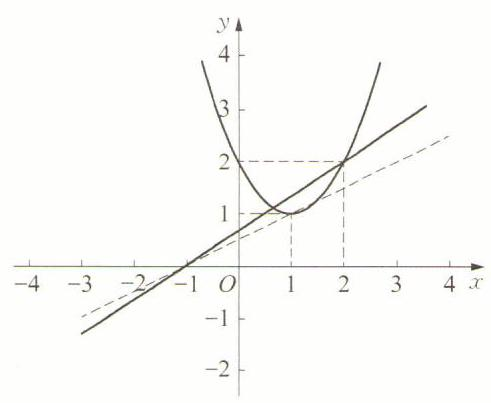
\includegraphics[max width=0.4\textwidth]{images/bo_d29ci7n7aajc738p8c80_6_1013_262_491_403_0.jpg}
\end{center}
\hspace*{3em} 

第 4 题图

令 $f\left( x\right)  = {x}^{2} - {2x} + 2,g\left( x\right)  = a\left( {x + 1}\right)$ ,所以 $A =$  $\{ x \mid  f\left( x\right)  < g\left( x\right) ,x \in  \mathbf{N}\} .$

如图所示,因为 $y = f\left( x\right)$ 是一个二次函数,其图象是确定的一条抛物线; 而 $y = g\left( x\right)$ 是一次函数,其图象是过一定点(-1,0)的动直线.

又 $x \in  \mathbf{N},a > 0$ ,数形结合得 $\dfrac{1}{2} < a \leq  \dfrac{2}{3}$ .

故实数 $a$ 的取值范围是 $\left( {\dfrac{1}{2},\dfrac{2}{3}}\right\rbrack$ .

5.【答案】[-5,3) ${U}\left( {4,5}\right)$

【解析】不等式 ${x}^{2} - {2x} - 8 > 0$ 的解集为 $\{ x \mid  x <  - 2$ 或 $x > 4\}$ .

不等式 $2{x}^{2} + \left( {{2k} + 7}\right) x + {7k} < 0$ 化为 $\left( {x + k}\right) \left( {x + \dfrac{7}{2}}\right)  < 0$ .

当 $k > \dfrac{7}{2}$ 时,不等式 $2{x}^{2} + \left( {{2k} + 7}\right) x + {7k} < 0$ 的解集为 $\left\{  {x - k < x <  - \dfrac{7}{2}}\right\}$ ,

由解集中的整数为-4,得 $- 5 \leq   - k <  - 4$ ,解得 $4 < k \leq  5$ .

当 $k < \dfrac{7}{2}$ 时,不等式 $2{x}^{2} + \left( {{2k} + 7}\right) x + {7k} < 0$ 的解集为 $\left\{  {x\left| { - \dfrac{7}{2} < x <  - k}\right. }\right\}$ ,

由解集中的整数为-3,得 $- 3 <  - k \leq  5$ ,解得 $- 5 \leq  k < 3$ .

当 $k = \dfrac{7}{2}$ 时,不等式组的解集为 $\varnothing$ ,不符合题意.

综上,实数 $k$ 的取值范围是 $\left\lbrack  {-5,3)\cup (4,5}\right\rbrack$ .

6.【答案】 $\{ x \mid  x <  - 3\}$

【解析】因为 $\left( {a + b}\right) x + {2a} - {3b} < 0$ 的解集为 $\left\{  {x\left| {x <  - \dfrac{1}{3}}\right. }\right\}$ ,所以 $a + b > 0$ ,且 $x <$  $\dfrac{{3b} - {2a}}{a + b}$ ,得 $\dfrac{{3b} - {2a}}{a + b} =  - \dfrac{1}{3}$ ,即 $a = {2b}$ 且 $a > 0$ .

所求不等式 $\left( {a - {3b}}\right) x + b - {2a} > 0$ 转化为 $- x - 3 > 0$ ,得 $x <  - 3$ ,即不等式 $\left( {a - {3b}}\right) x +$  $b - {2a} > 0$ 的解集为 $\{ x \mid  x <  - 3\}$ .

7.【答案】D

【解析】令 $f\left( x\right)  = \dfrac{3}{4}{x}^{2} - {3x} + 4$ ,则 $f\left( x\right)  = \dfrac{3}{4}{\left( x - 2\right) }^{2} + 1$ . 选项 A: 因为 $f\left( x\right)  = \dfrac{3}{4}{\left( x - 2\right) }^{2} + 1$ ,所以 $f\left( x\right)  \geq  1 > b >$  $a$ ,所以 $a \leq  \dfrac{3}{4}{x}^{2} - {3x} + 4 \leq  b$ 的解集为 $\varnothing$ ,故 ${A}$ 错误； 选项 B: 作出 $f\left( x\right)$ 的图象如图所示,由图可知,当 $a = 2$ 时, 不等式的解集应该分割为两段,故 ${B}$ 错误;

\begin{center}
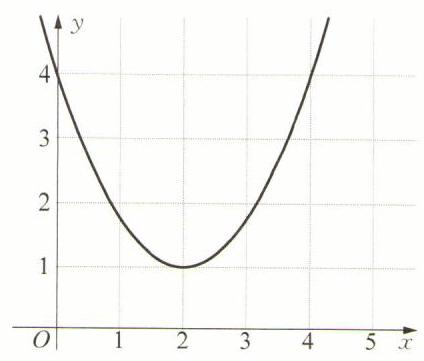
\includegraphics[max width=0.3\textwidth]{images/bo_d29ci7n7aajc738p8c80_7_1076_134_424_361_0.jpg}
\end{center}
\hspace*{3em} 

第 7 题图

选项 C、D:由 $f\left( x\right)$ 的图象易知,若不等式的解集为连续不

间断区间,则 $a \leq  1,b > 1$ ,若解集为 $\left\lbrack  {a,b}\right\rbrack$ ,则 $f\left( a\right)  = f\left( b\right)  = b$ ,且 $b > 2$ ,因为 $f\left( x\right)  =$  $\dfrac{3}{4}{\left( x - 2\right) }^{2} + 1$ ,所以 $f\left( b\right)  = \dfrac{3}{4}{\left( b - 2\right) }^{2} + 1 = b$ ,解得 $b = 4$ 或 $b = \dfrac{4}{3}$ ,因为 $b > 2$ ,所以 $b =$ 4,所以 $a = 0$ ,所以 $b - a = 4$ ,故 ${C}$ 错误, ${D}$ 正确.

8.【答案】①②

【解析】不等式 ${x}^{2} - {px} - {qx} + {pq} - 2 \leq  0$ 的解集为 $\left\lbrack  {m,n}\right\rbrack$ ,所以

\[
\left( {x - p}\right) \left( {x - q}\right)  \leq  2.
\]

(*)

对于 ①:代入 $x = \dfrac{1}{3}p + \dfrac{2}{3}q$ ,得 $\left( {\dfrac{2}{3}q - \dfrac{2}{3}p}\right) \left( {\dfrac{1}{3}p - \dfrac{1}{3}q}\right)  =  - \dfrac{2}{9}{\left( p - q\right) }^{2} < 0 \leq  2$ ,不等式成立,即 $\dfrac{1}{3}p + \dfrac{2}{3}q \in  \left\lbrack  {m,n}\right\rbrack$ ,故 ① 正确;

对于 ②: 因为 $m,n$ 为方程 ${x}^{2} - {px} - {qx} + {pq} - 2 = 0$ 的两个根,所以 $m + n = p + q,{mn} =$  ${pq} - 2$ ,所以 $\left( {m + 1}\right) \left( {n + 1}\right)  = {mn} + \left( {m + n}\right)  + 1 = {pq} - 2 + p + q + 1 = {pq} + p + q - 1$  $< \left( {p + 1}\right) \left( {q + 1}\right)$ ,故 ② 正确;

对于 ③: 因为 ${\left( n - m\right) }^{2} = {\left( m + n\right) }^{2} - {4mn} = {\left( p + q\right) }^{2} - {4pq} + 8 = {\left( q - p\right) }^{2} + 8$ ,所以 $n -$  $m = \sqrt{{\left( q - p\right) }^{2} + 8} \neq  q - p + 2\sqrt{2}$ ,故 ③ 错误;

对于④: ${m}^{3} + {n}^{3} = \left( {m + n}\right) \left( {{m}^{2} + {n}^{2} - {mn}}\right)  = \left( {m + n}\right) \left\lbrack  {{\left( m + n\right) }^{2} - {3mn}}\right\rbrack   = {\left( p + q\right) }^{3} - 3(p +$  $q)\left( {{pq} - 2}\right)  = {p}^{3} + {q}^{3} + 3{p}^{2}q + {3p}{q}^{2} - 3\left( {{p}^{2}q - {2p} + p{q}^{2} - {2q}}\right)  = {p}^{3} + {q}^{3} + 6\left( {p + q}\right)$ ,由于 $p + q$ 与 0 的关系不确定,故无法比较 ${m}^{3} + {n}^{3}$ 与 ${p}^{3} + {q}^{3}$ ,故 ④ 错误.

9.【答案】 $- \dfrac{1}{2}$ 与-2

【解析】由题意得, $f\left( x\right)  = \left| {x + 1}\right|  + \left| {{ax} + 1}\right|$ 的最小值为 $\dfrac{3}{2}$ . 因为 $f\left( x\right)$ 的图象是一条折线,所以 $f\left( x\right)$ 的最小值在折点处,即满足 $x + 1 = 0$ 或 ${ax} + 1 = 0$ ,函数 $f\left( x\right)$ 才可能取到最小值 $\dfrac{3}{2}$ ,当 $a = 0$ 时, $f\left( x\right)  = \left| {x + 1}\right|  + 1 \geq  1$ ,当 $x =  - 1$ 时, $f\left( x\right)$ 的最小值为

1,故 $a \neq  0$ .

① 当 $x =  - 1$ 时,则 $\left| {-a + 1}\right|  = \dfrac{3}{2}$ ,解得 $a =  - \dfrac{1}{2}$ 或 $\dfrac{5}{2}$ ,所以 $f\left( x\right)  = \left| {x + 1}\right|  + \left| {-\dfrac{1}{2}x + 1}\right|  \geq$

$\dfrac{3}{2}$ 或 $f\left( x\right)  = \left| {x + 1}\right|  + \left| {\dfrac{5x}{2} + 1}\right|  \geq  \dfrac{3}{5}$ ,因为 $f\left( x\right)$ 的最小值为 $\dfrac{3}{2}$ ,所以 $a =  - \dfrac{1}{2}$ .

② 当 $x =  - \dfrac{1}{a}$ 时,则 $\left| {-\dfrac{1}{a} + 1}\right|  = \dfrac{3}{2}$ ,解得 $a =  - 2$ 或 $\dfrac{2}{5}$ ,所以 $f\left( x\right)  = \left| {x + 1}\right|  + \left| {-{2x} + 1}\right|  \geq$

$\dfrac{3}{2}$ 或 $f\left( x\right)  = \left| {x + 1}\right|  + \left| {\dfrac{2}{5}x + 1}\right|  \geq  \dfrac{3}{5}$ ,所以 $a =  - 2$ .

综上所述, $a =  - \dfrac{1}{2}$ 或 $a =  - 2$ .

10.【答案】[2,4)

【解析】由 $4{\left\lbrack  x\right\rbrack  }^{2} - {20}\left\lbrack  x\right\rbrack   + {21} < 0$ ,得 $\dfrac{3}{2} < \left\lbrack  x\right\rbrack   < \dfrac{7}{2}$ ,由 $\left\lbrack  x\right\rbrack$ 表示整数,则 $\left\lbrack  x\right\rbrack   = 2,3$ ,

所以 $2 \leq  x < 4$ ,即解集为 $\lbrack 2,4)$ .

\section*{03 不等式的最值问题}

1.【答案】 $2\sqrt{3}$

【解析】直线 ${ax} - {by} - 3 = 0$ 过点(1, - 1),则 $a + b = 3$ .

又 $a > 0,b > 0$ ,设 $t = \sqrt{a + 1} + \sqrt{b + 2}$ ,则 $t > 0,{t}^{2} = a + 1 + b + 2 + 2\sqrt{\left( {a + 1}\right) \left( {b + 2}\right) } =$  $6 + 2\sqrt{\left( {a + 1}\right) \left( {b + 2}\right) }$ .

由 $\left( {a + 1}\right) \left( {b + 2}\right)  \leq  {\left( \dfrac{a + 1 + b + 2}{2}\right) }^{2} = 9$ ,当且仅当 $a + 1 = b + 2$ ,即 $a = 2,b = 1$ 时等号成立,所以 ${t}^{2} = 6 + 2\sqrt{\left( {a + 1}\right) \left( {b + 2}\right) } \leq  {12}$ ,即 $t \leq  2\sqrt{3}$ ,得 $\sqrt{a + 1} + \sqrt{b + 2}$ 的最大值为 $2\sqrt{3}$ ,当且仅当 $a = 2,b = 1$ 时等号成立.

2.【答案】D

【解析】由正实数 $x\text{ 、 }y\text{ 、 }z$ 满足 ${x}^{2} - {3xy} + 4{y}^{2} - z = 0$ ,所以 $z = {x}^{2} - {3xy} + 4{y}^{2}$ ,所以 $\dfrac{xy}{z} =$  $\dfrac{xy}{{x}^{2} - {3xy} + 4{y}^{2}} = \dfrac{1}{\dfrac{x}{y} + \dfrac{4y}{x} - 3} \leq  \dfrac{1}{2\sqrt{\dfrac{x}{y} \cdot  \dfrac{4y}{x}} - 3} = 1$ ,当且仅当 $x = {2y} > 0$ 时取等号,此时

$z = 2{y}^{2}$ . 所以 $\dfrac{2}{x} + \dfrac{1}{y} - \dfrac{2}{z} = \dfrac{2}{2y} + \dfrac{1}{y} - \dfrac{2}{2{y}^{2}} =  - {\left( \dfrac{1}{y} - 1\right) }^{2} + 1 \leq  1$ ,当且仅当 $y = 1$ 时取等号,

即 $\dfrac{2}{x} + \dfrac{1}{y} - \dfrac{2}{z}$ 的最大值是 1.

3.【答案】B

【解析】由 ${ab} + {2a} - 2 = 0$ ,得 $a = \dfrac{2}{b + 2}$ ,所以 ${4a} + b = \dfrac{8}{b + 2} + b = \dfrac{8}{b + 2} + \left( {b + 2}\right)  - 2 \geq$  $2\sqrt{\dfrac{8}{b + 2} \cdot  \left( {b + 2}\right) } - 2 = 4\sqrt{2} - 2$ ,当且仅当 $a = \dfrac{2}{b + 2},\dfrac{8}{b + 2} = b + 2$ ,即 $a = \dfrac{\sqrt{2}}{2},b = 2\sqrt{2} -$ 2 取等号.

4.【答案】2

【解析】由 ${\left( x - y\right) }^{2} = {\left( xy\right) }^{3}$ ,且 $x,y \in  {\mathbf{R}}^{ + }$ ,两边同除以 ${\left( xy\right) }^{2}$ ,得 ${\left( \dfrac{1}{y} - \dfrac{1}{x}\right) }^{2} = {xy}$ . 因为 ${\left( \dfrac{1}{x} + \dfrac{1}{y}\right) }^{2} = {\left( \dfrac{1}{y} - \dfrac{1}{x}\right) }^{2} + 4\dfrac{1}{xy} = {xy} + 4\dfrac{1}{xy} \geq  2\sqrt{{xy} \cdot  4\dfrac{1}{xy}} = 4$ ,当且仅当 ${xy} = 4\dfrac{1}{xy}$ , 即 $\left\{  \begin{array}{l} x = 2 + \sqrt{2}, \\  y = 2 - \sqrt{2} \end{array}\right.$ 或 $\left\{  \begin{array}{l} x = 2 - \sqrt{2}, \\  y = 2 + \sqrt{2} \end{array}\right.$ 时等号成立,所以 $\dfrac{1}{x} + \dfrac{1}{y} \geq  \sqrt{4} = 2$ ,即所求最小值为 2.

5.【答案】 $\left\lbrack  {\dfrac{2}{3},\dfrac{\sqrt{2}}{2}}\right\rbrack$

【解析】由题意 $a > 0,b > 0,4{a}^{2} + {b}^{2} - {2ab} = 2$ ,得 ${ab} = \dfrac{{\left( 2a + b\right) }^{2} - 2}{6} > 0$ ,则 ${2a} + b >$  $\sqrt{2}$ .

因为 ${\left( 2a + b\right) }^{2} = 2 + {6ab} \leq  2 + 3 \times  {\left( \dfrac{{2a} + b}{2}\right) }^{2}$ ,当且仅当 $b = {2a} = \sqrt{2}$ 时取等号,所以 $0 <$

${2a} + b \leq  2\sqrt{2}$ ,故 $\sqrt{2} < {2a} + b \leq  2\sqrt{2}$ .

因为 $\dfrac{{ab} + 1}{{2a} + b} = \dfrac{1}{6}\left( {{2a} + b + \dfrac{4}{{2a} + b}}\right)$ ,令 $t = {2a} + b,t \in  \left( {\sqrt{2},2\sqrt{2}}\right\rbrack$ ,所以原式 $= f\left( t\right)  =$  $\dfrac{1}{6}\left( {t + \dfrac{4}{t}}\right)  \geq  \dfrac{2}{3}$ ,当且仅当 $t = 2$ 取等号.

由对勾函数性质可知, $f{\left( t\right) }_{\min } = f\left( 2\right)  = \dfrac{2}{3}$ ,而 $f\left( \sqrt{2}\right)  = \dfrac{\sqrt{2}}{2},f\left( {2\sqrt{2}}\right)  = \dfrac{\sqrt{2}}{2}$ ,故 $f\left( t\right)  \in$  $\left\lbrack  {\dfrac{2}{3},\dfrac{\sqrt{2}}{2}}\right\rbrack$ ,即 $\dfrac{{ab} + 1}{{2a} + b} \in  \left\lbrack  {\dfrac{2}{3},\dfrac{\sqrt{2}}{2}}\right\rbrack$ .

6.【答案】D

【解析】解法一: (平均值不等式) 设 $c = \sqrt{3}a - b$ ,则 $\sqrt{3}{a}^{2} - {ab} = a\left( {\sqrt{3}a - b}\right)  = {ac}$ ,条件 ${a}^{2} +$

${b}^{2} - \sqrt{3}{ab} = 1 \Leftrightarrow  {a}^{2} + {c}^{2} - \sqrt{3}{ac} = 1$ ,所以 $\sqrt{3}{ac} + 1 = {a}^{2} + {c}^{2} \geq  {2ac}$ ,即 ${ac} \leq  2 + \sqrt{3}$ .

解法二: (三角换元) 由条件 ${\left( a - \dfrac{\sqrt{3}}{2}b\right) }^{2} + \dfrac{1}{4}{b}^{2} = 1$ ,可设 $\left\{  \begin{array}{l} a - \dfrac{\sqrt{3}}{2}b = \cos \theta , \\  \dfrac{b}{2} = \sin \theta , \end{array}\right.$ 即 $\left\{  \begin{array}{l} a = \cos \theta  + \sqrt{3}\sin \theta , \\  b = 2\sin \theta . \end{array}\right.$ 由于 $a > 0,b > 0$ ,故 $\left\{  \begin{array}{l} \cos \theta  + \sqrt{3}\sin \theta  > 0, \\  2\sin \theta  > 0, \end{array}\right.$ 解得 $0 < \theta  < \dfrac{5\pi }{6}$ ,所以 $\left\{  {\begin{array}{l} a = \cos \theta  + \sqrt{3}\sin \theta , \\  b = 2\sin \theta  \end{array}\left( {0 < \theta  < \dfrac{5\pi }{6}}\right) \text{ ,所以 }\sqrt{3}{a}^{2} - {ab} = \sqrt{3} + 2\sin {2\theta } \leq  2 + \sqrt{3}\text{ ,当且仅当 }\theta  = }\right.$  $\dfrac{\pi }{4}$ 时取等号.

7.【答案】 $2 + 2\sqrt{2}$

【解析】由题意, $a > 0,b > 0,c > 0,a + b + c = 2$ ,得 $a + b = 2 - c$ . 设 $2 - c = m,c = n\left( {m > 0,n > 0}\right)$ ,则 $m + n = 2$ ,得 $\dfrac{4}{a + b} + \dfrac{a + b}{c} = \dfrac{4}{2 - c} + \dfrac{2 - c}{c} = \dfrac{4}{2 - c} +$  $\dfrac{2}{c} - 1 = \dfrac{4}{m} + \dfrac{2}{n} - 1 = \dfrac{m + n}{2} \times  \left( {\dfrac{4}{m} + \dfrac{2}{n}}\right)  - 1 = 3 + \dfrac{2n}{m} + \dfrac{m}{n} - 1 \geq  2 + 2\sqrt{\dfrac{2n}{m} \cdot  \dfrac{m}{n}} = 2 + 2\sqrt{2},$ 当且仅当 ${m}^{2} = 2{n}^{2}$ ,即 $m = 4 - 2\sqrt{2},n = c = 2\sqrt{2} - 2$ 时取得等号,故 $\dfrac{4}{a + b} + \dfrac{a + b}{c}$ 的最小值为 $2 + 2\sqrt{2}$ .

8.【答案】 $\dfrac{3 + 2\sqrt{2}}{5}$

【解析】令 $a + {2b} = \lambda \left( {{3a} + {4b}}\right)  + \mu \left( {a + {3b}}\right)  = \left( {{3\lambda } + \mu }\right) a + \left( {{4\lambda } + {3\mu }}\right) b$ ,由 $\left\{  \begin{array}{l} {3\lambda } + \mu  = 1, \\  {4\lambda } + {3\mu } = 2 \end{array}\right.$ 得

$\left\{  \begin{array}{l} \lambda  = \dfrac{1}{5}, \\  \mu  = \dfrac{2}{5}, \end{array}\right.$ 则 $a + {2b} = \dfrac{1}{5}\left( {{3a} + {4b}}\right)  + \dfrac{2}{5}\left( {a + {3b}}\right)$ . 所以

\[
\dfrac{1}{{3a} + {4b}} + \dfrac{1}{a + {3b}} = \left( {\dfrac{1}{{3a} + {4b}} + \dfrac{1}{a + {3b}}}\right)  \cdot  \left\lbrack  {\dfrac{1}{5}\left( {{3a} + {4b}}\right)  + \dfrac{2}{5}\left( {a + {3b}}\right) }\right\rbrack
\]

\[
= \dfrac{3}{5} + \dfrac{1}{5}\left\lbrack  {\dfrac{2\left( {a + {3b}}\right) }{{3a} + {4b}} + \dfrac{{3a} + {4b}}{a + {3b}}}\right\rbrack   \geq  \dfrac{3}{5} + \dfrac{2}{5}\sqrt{\dfrac{2\left( {a + {3b}}\right) }{{3a} + {4b}} \cdot  \dfrac{{3a} + {4b}}{a + {3b}}} = \dfrac{3 + 2\sqrt{2}}{5},
\]

当且仅当 $\left\{  \begin{array}{l} a + {2b} = 1, \\  \dfrac{2\left( {a + {3b}}\right) }{{3a} + {4b}} = \dfrac{{3a} + {4b}}{a + {3b}} \end{array}\right.$ 时等号成立,即 $\dfrac{1}{{3a} + {4b}} + \dfrac{1}{a + {3b}}$ 的最小值是 $\dfrac{3 + 2\sqrt{2}}{5}$ .

9.【答案】 $\dfrac{1}{6}$

【解析】令 $m = x + 1,n = y + 2$ ,则 $x = m - 1,y = n - 2$ ,则 $x + {2y} = m - 1 + 2\left( {n - 2}\right)  =$ 1,即 $m + {2n} = 6$ ,得 $\dfrac{{x}^{2}}{x + 1} + \dfrac{2{y}^{2}}{y + 2} = \dfrac{{\left( m - 1\right) }^{2}}{m} + \dfrac{2{\left( n - 2\right) }^{2}}{n} = m + {2n} + \dfrac{1}{m} + \dfrac{8}{n} - {10} = \dfrac{1}{m} +$  $\dfrac{8}{n} - 4 = \dfrac{1}{6}\left( {\dfrac{1}{m} + \dfrac{8}{n}}\right) \left( {m + {2n}}\right)  - 4 = \dfrac{1}{6}\left( {\dfrac{2n}{m} + \dfrac{8m}{n} + {17}}\right)  - 4 \geq  \dfrac{1}{6}\left( {2\sqrt{\dfrac{2n}{m} \cdot  \dfrac{8m}{n}} + {17}}\right)  - 4 = \dfrac{1}{6},$ 当且仅当 $\dfrac{2n}{m} = \dfrac{8m}{n}$ ,即 $m = \dfrac{6}{5},n = \dfrac{12}{5}$ 时等号成立,故 $\dfrac{{x}^{2}}{x + 1} + \dfrac{2{y}^{2}}{y + 2}$ 的最小值为 $\dfrac{1}{6}$ .

10.【答案】 $\dfrac{4}{5}$

【解析】根据题意,若 ${2x} + y = 2$ ,则 $\dfrac{4{x}^{2}}{y + 1} + \dfrac{{y}^{2}}{{2x} + 2} = \dfrac{{\left( 2 - y\right) }^{2}}{y + 1} + \dfrac{{\left( 2 - 2x\right) }^{2}}{2\left( {x + 1}\right) } =$  $\dfrac{{\left\lbrack  \left( y + 1\right)  - 3\right\rbrack  }^{2}}{y + 1} + 2\dfrac{{\left\lbrack  \left( x + 1\right)  - 2\right\rbrack  }^{2}}{x + 1} = \left( {y + 1}\right)  + \dfrac{9}{y + 1} + 2\left( {x + 1}\right)  + \dfrac{16}{2\left( {x + 1}\right) } - {14} = \dfrac{9}{y + 1} +$  $\dfrac{16}{2\left( {x + 1}\right) } - 9$ ; 又由 ${2x} + y = 2$ ,则有 $2\left( {x + 1}\right)  + \left( {y + 1}\right)  = 5$ ,则 $\dfrac{4{x}^{2}}{y + 1} + \dfrac{{y}^{2}}{{2x} + 2} =$  $\left\lbrack  {\dfrac{9}{y + 1} + \dfrac{16}{2\left( {x + 1}\right) }}\right\rbrack  \dfrac{\left( {{2x} + 2}\right)  + \left( {y + 1}\right) }{5} - 9 = \dfrac{1}{5}\left\lbrack  {{16} + 9 + \dfrac{{18}\left( {x + 1}\right) }{y + 1} + \dfrac{8\left( {y + 1}\right) }{x + 1}}\right\rbrack   - 9 \geq$  $\dfrac{1}{5}\left\lbrack  {{25} + 2\sqrt{\dfrac{{18}\left( {x + 1}\right) }{y + 1} \times  \dfrac{8\left( {y + 1}\right) }{x + 1}}}\right\rbrack   - 9 = \dfrac{4}{5}$ ,当且仅当 $y + 1 = \dfrac{3}{2}\left( {x + 1}\right)  = \dfrac{15}{7}$ 时等号成立, 即 $\dfrac{4{x}^{2}}{y + 1} + \dfrac{{y}^{2}}{{2x} + 2}$ 的最小值是 $\dfrac{4}{5}$ .

11.【答案】 ${C}$

【解析】由 $x > 0,y > 0$ 且 $\dfrac{2}{x} + \dfrac{1}{y} = 1$ ,可得 ${xy} = x + {2y}$ ,所以 ${4xy} - {3x} - {6y} = {4x} + {8y} -$  ${3x} - {6y} = x + {2y} = \left( {\dfrac{2}{x} + \dfrac{1}{y}}\right) \left( {x + {2y}}\right)  = 4 + \dfrac{4y}{x} + \dfrac{x}{y} \geq  4 + 2\sqrt{\dfrac{4y}{x} \cdot  \dfrac{x}{y}} = 8$ ,当且仅当 $\dfrac{4y}{x} =$  $\dfrac{x}{y}$ ,即 $x = 4,y = 2$ 时取等号.

12.【答案】B

【解析】由 $\left\{  {a}_{n}\right\}$ 是等差数列,得 ${S}_{2013} = \dfrac{2013}{2}\left( {{a}_{1} + {a}_{2013}}\right)  = {2013}$ ,解得 ${a}_{1} + {a}_{2013} = 2$ ,于是 ${a}_{2} +$  ${a}_{2012} = {a}_{1} + {a}_{2013} = 2$ ,所以 $\dfrac{1}{{a}_{2}} + \dfrac{1}{{a}_{2012}} = \dfrac{1}{2}\left( {{a}_{2} + {a}_{2012}}\right) \left( {\dfrac{1}{{a}_{2}} + \dfrac{1}{{a}_{2012}}}\right)  = 1 + \dfrac{1}{2}\left( {\dfrac{{a}_{2012}}{{a}_{2}} + \dfrac{{a}_{2}}{{a}_{2012}}}\right)  \geq  1 +$

$\dfrac{1}{2} \times  2\sqrt{\dfrac{{a}_{2012}}{{a}_{2}} \cdot  \dfrac{{a}_{2}}{{a}_{2012}}} = 2$ ,当且仅当 ${a}_{2} = {a}_{2012} = 1$ 时,等号成立,所以 $\dfrac{1}{{a}_{2}} + \dfrac{1}{{a}_{2012}}$ 的最小值为 2 .

13.【答案】A

【解析】由 ${2a} + b = 3$ ,得 $\left( {{2a} - 1}\right)  + \left( {b - 1}\right)  = 1$ .

因为 $a > \dfrac{1}{2},b > 1$ ,所以 ${2a} - 1 > 0,b - 1 > 0$ .

又 $\dfrac{2a}{{2a} - 1} + \dfrac{b}{b - 1} = \dfrac{{2a} - 1 + 1}{{2a} - 1} + \dfrac{b - 1 + 1}{b - 1} = 2 + \dfrac{1}{{2a} - 1} + \dfrac{1}{b - 1}$ ,所以 $\dfrac{1}{{2a} - 1} + \dfrac{1}{b - 1} =$

$\left( {\dfrac{1}{{2a} - 1} + \dfrac{1}{b - 1}}\right) \left\lbrack  {\left( {{2a} - 1}\right)  + \left( {b - 1}\right) }\right\rbrack   = 2 + \dfrac{{2a} - 1}{b - 1} + \dfrac{b - 1}{{2a} - 1} \geq  2 + 2\sqrt{\dfrac{{2a} - 1}{b - 1} \times  \dfrac{b - 1}{{2a} - 1}} =$

$2 + 2 = 4$ ,当且仅当 $\left\{  \begin{array}{l} {2a} + b = 3, \\  \dfrac{{2a} - 1}{b - 1} = \dfrac{b - 1}{{2a} - 1}, \end{array}\right.$ 即 $a = \dfrac{3}{4},b = \dfrac{3}{2}$ 时取等号.

所以, $\dfrac{2a}{{2a} - 1} + \dfrac{b}{b - 1} = 2 + \dfrac{1}{{2a} - 1} + \dfrac{1}{b - 1} \geq  6$ .

14.【答案】B

【解析】由已知,得 $\left( {1 + \dfrac{1}{a}}\right) \left( {1 + \dfrac{8}{b}}\right)  = \left( {1 + \dfrac{a + b}{a}}\right) \left( {1 + \dfrac{{8a} + {8b}}{b}}\right)  = \left( {2 + \dfrac{b}{a}}\right) \left( {9 + \dfrac{8a}{b}}\right)  = {26} +$

$\dfrac{9b}{a} + \dfrac{16a}{b} \geq  {26} + 2\sqrt{\dfrac{9b}{a} \cdot  \dfrac{16a}{b}} = {50}$ ,当且仅当 $\dfrac{9b}{a} = \dfrac{16a}{b}$ ,即 $a = \dfrac{3}{7},b = \dfrac{4}{7}$ 时等号成立.

因此, $\left( {1 + \dfrac{1}{a}}\right) \left( {1 + \dfrac{8}{b}}\right)$ 的最小值是 50.

15.【答案】9

【解析】由 ${ab} - a - b = 0$ 得 $\dfrac{1}{a} + \dfrac{1}{b} = 1$ ,所以 ${4a} + b = \left( {{4a} + b}\right) \left( {\dfrac{1}{a} + \dfrac{1}{b}}\right)  = 5 + \dfrac{b}{a} + \dfrac{4a}{b} \geq  5 +$  $2\sqrt{4} = 9$ ,当且仅当 $\dfrac{b}{a} = \dfrac{4a}{b}$ ,即 $a = \dfrac{3}{2},b = 3$ 时取等号,故 ${4a} + b$ 的最小值为 9 .

16.【答案】[-2,4]

【解析】由于 $0 < m < \dfrac{1}{2}$ ,所以 $\dfrac{1}{2} \cdot  {2m} \cdot  \left( {1 - {2m}}\right)  \leq  \dfrac{1}{2} \cdot  {\left\lbrack  \dfrac{{2m} + \left( {1 - {2m}}\right) }{2}\right\rbrack  }^{2} = \dfrac{1}{8}$ ,当且仅当 ${2m} = 1 - {2m}$ ,即 $m = \dfrac{1}{4}$ 时取等号,所以 $\dfrac{1}{m} + \dfrac{2}{1 - {2m}} = \dfrac{1}{m\left( {1 - {2m}}\right) } \geq  8$ ,因为 $\dfrac{1}{m} +$  $\dfrac{2}{1 - {2m}} \geq  {k}^{2} - {2k}$ 恒成立,所以 ${k}^{2} - {2k} - 8 \leq  0$ ,所以 $- 2 \leq  k \leq  4$ ,所以实数 $k$ 的取值范围为 $\left\lbrack  {-2,4}\right\rbrack$ .

17.【答案】 $\lbrack  - 1, + \infty )$

【解析】由题意得不等式 ${xy} \leq  a{x}^{2} + 2{y}^{2}$ 对于 $x \in  \left\lbrack  {1,2}\right\rbrack  ,y \in  \left\lbrack  {2,3}\right\rbrack$ 恒成立,即 $a \geq  \dfrac{y}{x} -$  $2{\left( \dfrac{y}{x}\right) }^{2}$ ,对于 $x \in  \left\lbrack  {1,2}\right\rbrack  ,y \in  \left\lbrack  {2,3}\right\rbrack$ 恒成立,令 $t = \dfrac{y}{x}$ ,则 $1 \leq  t \leq  3$ ,所以 $a \geq  t - 2{t}^{2}$ 在

[1,3] 上恒成立,因为 $f\left( t\right)  =  - 2{t}^{2} + t =  - 2{\left( t - \dfrac{1}{4}\right) }^{2} + \dfrac{1}{8}$ ,所以 $f{\left( t\right) }_{\max } =  - 1$ ,所以 $a \geq$ -1,所以实数 $a$ 的取值范围是 $\lbrack  - 1, + \infty )$ .

18.【答案】A

【解析】 $k$ 可以取 $- 2\text{ 、 } - \dfrac{2}{3}\text{ 、 }0\text{ 、 }\dfrac{2}{3}$ 四个值,使得 $x \in  \left( {-1,0}\right)  \cup  \left( {0,1}\right)$ 时,均有 ${x}^{k} > \left| x\right|$ 成立.

\section*{函数}

\section*{04 函数的定义}

1.【答案】27

【解析】因为对应关系为 $y = {x}^{2} - 1$ ,值域为 $\{ 0,3,8\}$ ,所以由 ${x}^{2} - 1 = 0 \Rightarrow  x =  \pm  1,{x}^{2} - 1 =$  $3 \Rightarrow  x =  \pm  2,{x}^{2} - 1 = 8 \Rightarrow  x =  \pm  3$ 知,要构成满足条件的函数,定义域应该由 $\pm  1, \pm  2, \pm  3$ 这三组数所构成,且 $\pm  1, \pm  2, \pm  3$ 这三组数中,每组的两个数至少要取一个,所以满足题意的定义域可以有 $3 \times  3 \times  3 = {27}$ (种),即所求的 “同族函数” 有 27 个.

2.【答案】A

【解析】因为 $\{ \left( {x,y}\right)  \mid  y = f\left( x\right) ,a \leq  x \leq  b\}  \cap  \{ \left( {x,y}\right)  \mid  x = 0\}$ 只有一个子集,所以 $\{ \left( {x,y}\right)  \mid  y = f\left( x\right) ,a \leq  x \leq  b\}  \cap  \{ \left( {x,y}\right)  \mid  x = 0\}$ 为空集, $\{ \left( {x,y}\right)  \mid  x = 0\}$ 是由所有横坐标为 0 的点组成的集合,说明 $\{ \left( {x,y}\right)  \mid  y = f\left( x\right) ,a \leq  x \leq  b\}$ 中没有横坐标为 0 的点,所以由函数的定义可知 $0 \notin  \left\lbrack  {a,b}\right\rbrack$ ,所以 $a\text{ 、 }b$ 同号.

3.【答案】B

【解析】对于 ${A}$ ,当 $x = \dfrac{\pi }{4}$ 时,有 $f\left( {\cos \left( {2 \cdot  \dfrac{\pi }{4}}\right) }\right)  = f\left( 0\right)  = \sin \dfrac{\pi }{4} = \dfrac{\sqrt{2}}{2}$ ; 当 $x =  - \dfrac{\pi }{4}$ 时,有

$f\left( {\cos \left( {2 \cdot  \dfrac{-\pi }{4}}\right) }\right)  = f\left( 0\right)  = \sin \left( {-\dfrac{\pi }{4}}\right)  =  - \dfrac{\sqrt{2}}{2}$ ,得出的 $f\left( 0\right)$ 的值相互矛盾,故不存在这样的函数满足选项 ${A}$ 的性质,即选项 ${A}$ 错误；同理可推出选项 ${C}$ 、 ${D}$ 也错误；对于 ${B}$ , $f\left( {{x}^{2} - }\right.$  ${2x}) = f\left\lbrack  {{\left( x - 1\right) }^{2} - 1}\right\rbrack   = \left| {x - 1}\right|  \Rightarrow  f\left( {{\left| x - 1\right| }^{2} - 1}\right)  = \left| {x - 1}\right|  \Rightarrow  f\left( {{\left| x - 1\right| }^{2} - 1}\right)  =$  $\left| {x - 1}\right|  = \sqrt{\left( {{\left| x - 1\right| }^{2} - 1}\right)  + 1}$ . 显然函数 $f\left( x\right)  = \sqrt{x + 1}\left( {x \geq   - 1}\right)$ 满足选项 ${B}$ 的性质.

4.【答案】 $\left\lbrack  {0,\dfrac{\pi }{3}}\right\rbrack   \cup  \left\lbrack  {\dfrac{2\pi }{3},\pi }\right\rbrack$

【解析】 $f\left( x\right)$ 的图象为如图 1 所示的一段弧,弧所在的圆的方程为: ${x}^{2} + {y}^{2} = 1$ ,其中 $A\left( {-\dfrac{1}{2},\dfrac{\sqrt{3}}{2}}\right) ,B\left( {\dfrac{1}{2},\dfrac{\sqrt{3}}{2}}\right)$ . 在图象绕原点旋转的过程中,当 $B$ 从图 1 的位置旋转到 (1,0) 前(含),如图 2 所示,根据函数的定义,任意竖线与图象最多只有 1 个交点,在这个旋转过程所得的图形均为函数的图象,故 $0 \leq  \theta  \leq  \dfrac{\pi }{3}$ 满足要求. 在图象绕原点旋转的过程中,当 $B$ 从图 2 的 (1,0) 位置旋转到 $x$ 轴下方,而 $A$ 在 $x$ 轴上,如图 3 所示,根据函数的定义,在这个旋转过程所得的图形不是函数的图象,故 $\dfrac{\pi }{3} < \theta  < \dfrac{2\pi }{3}$ 不符合. 当 $A$ 旋转到 $x$ 轴下方时,如图 4 所示,根据函数的定义,在这个旋转过程所得的图形又是函数的图象了,故 $\dfrac{2\pi }{3} \leq  \theta  \leq  \pi$ 符合.

\begin{center}
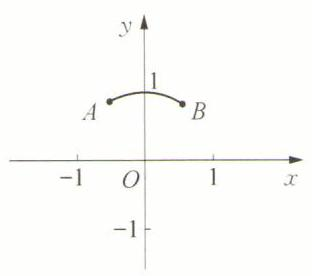
\includegraphics[max width=0.2\textwidth]{images/bo_d29ci7n7aajc738p8c80_14_157_1324_312_276_0.jpg}
\end{center}
\hspace*{3em} 

第 4 题图 1

\begin{center}
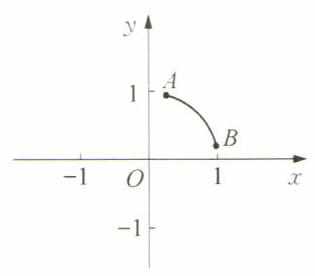
\includegraphics[max width=0.2\textwidth]{images/bo_d29ci7n7aajc738p8c80_14_494_1324_315_276_0.jpg}
\end{center}
\hspace*{3em} 

第 4 题图 2

\begin{center}
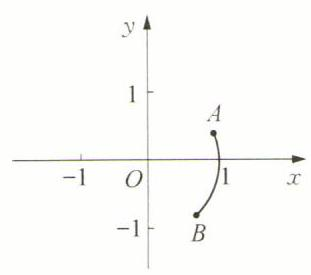
\includegraphics[max width=0.2\textwidth]{images/bo_d29ci7n7aajc738p8c80_14_836_1322_311_275_0.jpg}
\end{center}
\hspace*{3em} 

第 4 题图 3

\begin{center}
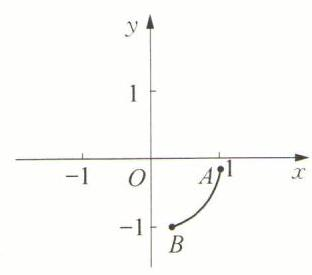
\includegraphics[max width=0.2\textwidth]{images/bo_d29ci7n7aajc738p8c80_14_1174_1321_312_275_0.jpg}
\end{center}
\hspace*{3em} 

第 4 题图 4

5.【答案】B

【解析】由题意可得:问题相当于圆上以 6 个点为一组,每次绕原点逆时针旋转 $\dfrac{\pi }{3}$ 个单位后与下一个点会重合. 假设 ${A}_{1}$ 为函数图象上的任意一点.

因为 $f\left( x\right)$ 的图象绕原点逆时针旋转 $\dfrac{\pi }{3}$ 后与原图象重合,所以旋转后 ${A}_{1}$ 的对应点 ${A}_{2}$ 也在 $f\left( x\right)$ 的图象上,同理 ${A}_{2}$ 的对应点 ${A}_{3}$ 也在图象上,以此类推, $f\left( x\right)$ 对应的图象可以为一个

圆周上 6 等分的 6 个点. 当 $f\left( 1\right)  = \sqrt{3}$ 时,即 ${A}_{1}\left( {1,\sqrt{3}}\right)$ ,如图所示,此时 ${A}_{5}\left( {1, - \sqrt{3}}\right)$ ,不满足函数定义; 当 $f\left( 1\right)  = \dfrac{\sqrt{3}}{3}$ 时, 即 ${A}_{1}\left( {1,\dfrac{\sqrt{3}}{3}}\right)$ ,此时 ${A}_{6}\left( {1, - \dfrac{\sqrt{3}}{3}}\right)$ ,不满足函数定义; 当 $f\left( 1\right)  = 0$ 时,即 ${A}_{6}\left( {1,0}\right)$ ,此时 ${A}_{1}\left( {\dfrac{1}{2},\dfrac{\sqrt{3}}{2}}\right) ,{A}_{5}\left( {\dfrac{1}{2}, - \dfrac{\sqrt{3}}{2}}\right)$ , 不满足函数定义.

\begin{center}
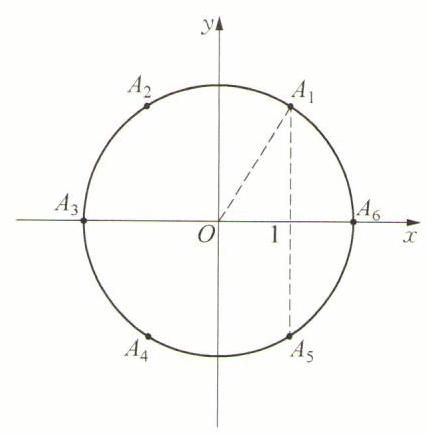
\includegraphics[max width=0.3\textwidth]{images/bo_d29ci7n7aajc738p8c80_15_1079_129_427_434_0.jpg}
\end{center}
\hspace*{3em} 

第 5 题图

6.【答案】(0,2)

\begin{center}
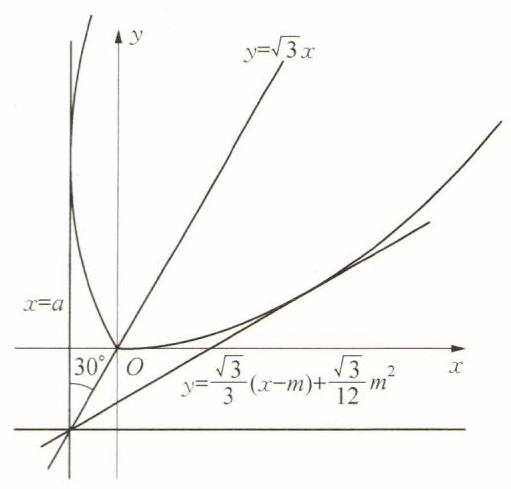
\includegraphics[max width=0.4\textwidth]{images/bo_d29ci7n7aajc738p8c80_15_995_643_511_489_0.jpg}
\end{center}
\hspace*{3em} 

第 6 题图

【解析】如图所示,设 $l$ 是 $f\left( x\right)  = \dfrac{\sqrt{3}}{12}{x}^{2}\left( {0 \leq  x \leq  m}\right)$ 在点 $M\left( {m,\dfrac{\sqrt{3}}{12}{m}^{2}}\right)$ 处的切线,因为曲线 $C$ 与函数 $f\left( x\right)  = \dfrac{\sqrt{3}}{12}{x}^{2}\left( {0 \leq  x \leq  m}\right)$ 的图象关于直线 $y = \sqrt{3}x$ 对称,所以直线 $l$ 关于 $y = \sqrt{3}x$ 对称后的直线为 $x = a$ 时曲线 $C$ 才能是某函数的图象. 直线 $y = \sqrt{3}x$ 与 $x = a$ 的夹角为 $\dfrac{\pi }{6}$ ,得 $l$ 的倾斜角为 $\dfrac{\pi }{6}$ ,所以 $l$ 的方程为 $y =$

$\dfrac{\sqrt{3}}{3}\left( {x - m}\right)  + \dfrac{\sqrt{3}}{12}{m}^{2}$ . 联立方程得 $\left\{  \begin{array}{l} y = \dfrac{\sqrt{3}}{3}\left( {x - m}\right)  + \dfrac{\sqrt{3}}{12}{m}^{2}, \\  y = \dfrac{\sqrt{3}}{12}{x}^{2}, \end{array}\right.$ 即 ${x}^{2} - {4x} + {4m} - {m}^{2} = 0$ ,所

以 $\Delta  = {16} - {16m} + 4{m}^{2} = 0$ ,解得 $m = 2$ (此处也可通过导数知识, ${f}^{\prime }\left( m\right)  = \dfrac{\sqrt{3}}{3}$ 解出 $m = 2$ ), 所以 $m$ 的取值范围为 $(0,2\rbrack$ .

7.【答案】 $\left\lbrack  {0,\dfrac{\pi }{4}}\right)$

\begin{center}
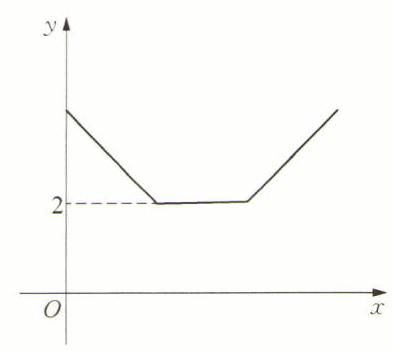
\includegraphics[max width=0.3\textwidth]{images/bo_d29ci7n7aajc738p8c80_15_1107_1684_393_351_0.jpg}
\end{center}
\hspace*{3em} 

第 7 题图

【解析】先画出函数 $y = \left| {\dfrac{1}{2}x - 1}\right|  + \left| {\dfrac{1}{2}x - 2}\right|  + 1$ 的图象,如图所示.

由图可知,当图象绕坐标原点顺时针方向旋转角大于等于 $\dfrac{\pi }{4}$ 时,曲线 $C$ 都不是一个函数的图象,则 $\theta$ 的取值范围是 $\left\lbrack  {0,\dfrac{\pi }{4}}\right)$ .

\section*{05 函数的值域与最值}

1.【答案】2035

【解析】设 $g\left( x\right)  = f\left( x\right)  - x$ ,则 $g\left( {2020}\right)  = g\left( {2021}\right)  = g\left( {2022}\right)  = 0$ ,所以 $g\left( x\right)  = 2(x -$ 2020) $\left( {x - {2021}}\right) \left( {x - {2022}}\right)$ ,所以 $g\left( {2023}\right)  = 2 \times  3 \times  2 \times  1 = {12}$ ,所以 $f\left( {2023}\right)  = {12} + {2023} =$ 2035.

2.【答案】(1) $\left\lbrack  {1,\dfrac{7}{3}}\right\rbrack  \left( 2\right) \lbrack 1,2) \cup  \lbrack 3, + \infty )$

【解析】(1) 函数的定义域是 $\mathbf{R},y = \dfrac{2\left( {{x}^{2} - x + 1}\right)  + x - 1}{{x}^{2} - x + 1} = 2 + \dfrac{x - 1}{{x}^{2} - x + 1}$ ,设 $x - 1 = t$ , $t \in  \mathbf{R},x = t + 1$ ,则 $y = 2 + \dfrac{t}{{t}^{2} + t + 1}$ . 当 $t \neq  0$ 时, $y = 2 + \dfrac{1}{t + \dfrac{1}{t} + 1}$ . 当 $t > 0$ 时, $t + \dfrac{1}{t} +$  $1 \geq  3$ ,得 $2 < y \leq  \dfrac{7}{3}$ ; 当 $t < 0$ 时, $t + \dfrac{1}{t} + 1 \leq   - 1$ ,得 $1 \leq  y < 2$ . 当 $t = 0$ 时, $y = 2$ . 综上: 函数的值域是 $\left\lbrack  {1,\dfrac{7}{3}}\right\rbrack$ .

(2)函数有意义,则 $4{x}^{2} - {8x} + 3 \geq  0$ ,解得 $x \geq  \dfrac{3}{2}$ 或 $x \leq  \dfrac{1}{2}$ ,即定义域是 $\left( {-\infty ,\dfrac{1}{2}}\right\rbrack   \cup$  $\left\lbrack  {\dfrac{3}{2}, + \infty }\right) ,y = {2x} - 2 + \sqrt{{\left( 2x - 2\right) }^{2} - 1} + 2$ ,设 ${2x} - 2 = t,t \leq   - 1$ 或 $t \geq  1,y = t +$  $\sqrt{{t}^{2} - 1} + 2$

当 $t \geq  1$ 时,函数是增函数, $t = 1$ 时,函数取得最小值 3,得 $y \geq  3$ ,即函数的值域是 $\lbrack 3$ , $+ \infty )$ ; 当 $t \leq   - 1$ 时, $y = t + \sqrt{{t}^{2} - 1} + 2 = \dfrac{1}{t - \sqrt{{t}^{2} - 1}} + 2$ ,函数是减函数,当 $t =  - 1$ 时, 取得最小值 1,当 $t \rightarrow   - \infty$ 时, $y \rightarrow  2$ ,即函数的值域是 $\lbrack 1,2)$ .

综上: 函数的值域是 $\lbrack 1,2) \cup  \lbrack 3, + \infty )$ .

【提示】此题也可通过三角换元来处理,设 ${2x} - 2 = \sec \theta ,\theta  \in  \left\lbrack  {0,\dfrac{\pi }{2}}\right)  \cup  \left\lbrack  {\pi ,\dfrac{3\pi }{2}}\right)$ ,进而求值域.

3.【答案】 $\lbrack  - 1, + \infty )$

【解析】由 $f\left( x\right)  = \left( {x + 1}\right) \left( {x + 2}\right) \left( {x + 3}\right) \left( {x + 4}\right)  = \left( {x + 1}\right) \left( {x + 4}\right) \left( {x + 2}\right) \left( {x + 3}\right)  = \left( {{x}^{2} + }\right.$  ${5x} + 4)\left( {{x}^{2} + {5x} + 6}\right)  = {\left( {x}^{2} + 5x\right) }^{2} + {10}\left( {{x}^{2} + {5x}}\right)  + {24} = {\left( {x}^{2} + 5x + 5\right) }^{2} - 1$ ,因为 ${x}^{2} +$  ${5x} + 5 = {\left( x + \dfrac{5}{2}\right) }^{2} - \dfrac{5}{4} \geq   - \dfrac{5}{4}$ ,得 ${\left( {x}^{2} + 5x + 5\right) }^{2} \geq  0$ ,所以 ${\left( {x}^{2} + 5x + 5\right) }^{2} - 1 \geq   - 1$ ,即 $f\left( x\right)$ 的值域是 $\lbrack  - 1, + \infty )$ .

4.【答案】 $\left\lbrack  {\dfrac{2\sqrt{6}}{3},\dfrac{5}{3}}\right\rbrack$

【解析】由正数 $x\text{ 、 }y\text{ 、 }z$ 满足 $\left( {x + {2y}}\right) \left( {y + z}\right)  = {4yz}$ ,得 $z = \dfrac{\left( {x + {2y}}\right) y}{{2y} - x}$ ,又由 $z =$  $\dfrac{\left( {x + {2y}}\right) y}{{2y} - x} > 0$ ,且 $x$ 、 $y$ 都为正数,得 ${2y} - x > 0$ . 又 $z \leq  {3x}$ ,则 $\dfrac{\left( {x + {2y}}\right) y}{{2y} - x} \leq  {3x}$ ,整理可得 $\dfrac{3{x}^{2} - {5xy} + 2{y}^{2}}{{2y} - x} \leq  0$ ,即 $\dfrac{\left( {{3x} - {2y}}\right) \left( {x - y}\right) }{{2y} - x} \leq  0$ . 因为 ${2y} - x > 0$ ,所以 $\left( {{3x} - {2y}}\right) (x -$  $y) \leq  0$ ,可得 $\left( {\dfrac{x}{y} - \dfrac{2}{3}}\right) \left( {\dfrac{x}{y} - 1}\right)  \leq  0$ ,令 $t = \dfrac{x}{y}$ ,则 $\dfrac{2}{3} \leq  t \leq  1$ ,于是 $P = \dfrac{3{x}^{2} + 2{y}^{2}}{3xy} = \dfrac{x}{y} + \dfrac{2}{3} \times$  $\dfrac{y}{x} = t + \dfrac{\dfrac{2}{3}}{t}$ 在 $\left\lbrack  {\dfrac{2}{3},\dfrac{\sqrt{6}}{3}}\right\rbrack$ 上单调递减,在 $\left\lbrack  {\dfrac{\sqrt{6}}{3},1}\right\rbrack$ 单调递增,当 $t = \dfrac{\sqrt{6}}{3}$ 时, $P$ 有最小值 $\dfrac{2\sqrt{6}}{3}$ ,当 $t = 1$ 或 $t = \dfrac{2}{3}$ 时, $P$ 有最大值 $\dfrac{5}{3}$ ,所以 $P$ 的取值范围是 $\left\lbrack  {\dfrac{2\sqrt{6}}{3},\dfrac{5}{3}}\right\rbrack$ .

5.【答案】 $\left\lbrack  {\dfrac{\sqrt{6}}{2},\dfrac{3\sqrt{2}}{2}}\right\rbrack$

【解析】解法一: 由已知得, $f\left( x\right)  = \sqrt{{2x} - 1} + \sqrt{2 - x},x \in  \left\lbrack  {\dfrac{1}{2},2}\right\rbrack$ ,构造函数 $h\left( x\right)  =$  $- \sqrt{4 - {2x}} + \sqrt{x - \dfrac{1}{2}},x \in  \left\lbrack  {\dfrac{1}{2},2}\right\rbrack$ ,则 $h\left( x\right)$ 在 $\left\lbrack  {\dfrac{1}{2},2}\right\rbrack$ 上单调递增,即可得 $h\left( x\right)  \in$  $\left\lbrack  {-\sqrt{3},\sqrt{\dfrac{3}{2}}}\right\rbrack$ ,因为 ${f}^{2}\left( x\right)  + {h}^{2}\left( x\right)  = \dfrac{9}{2}$ ,所以 ${f}^{2}\left( x\right)  = \dfrac{9}{2} - {h}^{2}\left( x\right)  \in  \left\lbrack  {\dfrac{3}{2},\dfrac{9}{2}}\right\rbrack$ ,所以 $f\left( x\right)  \in  \left\lbrack  {\dfrac{\sqrt{6}}{2},\dfrac{3\sqrt{2}}{2}}\right\rbrack  .$

解法二: $f\left( x\right)  = \sqrt{{2x} - 1} + \sqrt{2 - x} = \sqrt{2}\sqrt{x - \dfrac{1}{2}} + \sqrt{2 - x},x \in  \left\lbrack  {\dfrac{1}{2},2}\right\rbrack$ ,设 $\sqrt{x - \dfrac{1}{2}} = m$ , $\sqrt{2 - x} = n$ ,显然 ${m}^{2} + {n}^{2} = \dfrac{3}{2},m \in  \left\lbrack  {0,\dfrac{\sqrt{6}}{2}}\right\rbrack  ,n \in  \left\lbrack  {0,\dfrac{\sqrt{6}}{2}}\right\rbrack$ . 原式转化为求 $y = \sqrt{2}m + n$ 的范围,设 $m = \dfrac{\sqrt{6}}{2}\cos \theta ,n = \dfrac{\sqrt{6}}{2}\sin \theta \left( {\theta  \in  \left\lbrack  {0,\dfrac{\pi }{2}}\right\rbrack  }\right)$ ,即求 $y = \sqrt{2} \cdot  \dfrac{\sqrt{6}}{2}\cos \theta  + \dfrac{\sqrt{6}}{2}\sin \theta$ 的范围,此时 $y = \sqrt{2} \cdot  \dfrac{\sqrt{6}}{2}\cos \theta  + \dfrac{\sqrt{6}}{2}\sin \theta  = \dfrac{3\sqrt{2}}{2}\sin \left( {\theta  + \varphi }\right)$ ,其中 $\cos \varphi  = \dfrac{1}{\sqrt{3}},\sin \varphi  = \dfrac{2}{\sqrt{3}}$ ,易求得 $y = f\left( x\right)  \in  \left\lbrack  {\dfrac{\sqrt{6}}{2},\dfrac{3\sqrt{2}}{2}}\right\rbrack  .$

6.【答案】 $4\sqrt{5}$

【解析】因为 $y = \sqrt{{\left( x - 0\right) }^{2} + {\left( 0 - 3\right) }^{2}} + \sqrt{{\left( x - 4\right) }^{2} + {\left( 0 - 5\right) }^{2}}$ ,所以函数 $y$ 是 $x$ 轴上的点 $P\left( {x,0}\right)$ 与两定点 $A\left( {0,3}\right) \text{ 、 }B\left( {4,5}\right)$ 距离之和, $y$ 的最小值就是 $\left| {PA}\right|  + \left| {PB}\right|$ 的最小值, 通过在直角坐标系中作图可知,若 $A$ 关于 $x$ 轴的对称点为 ${A}^{\prime }\left( {0, - 3}\right) ,\left| {PA}\right|  + \left| {PB}\right|$ 的最小值等于 $\left| {{A}^{\prime }B}\right|$ ,即 $\sqrt{{\left( 4 - 0\right) }^{2} + {\left( 5 + 3\right) }^{2}} = 4\sqrt{5}$ ,所以 ${y}_{\min } = 4\sqrt{5}$ .

7.【答案】 ${21} - 6\sqrt{6}$

【解析】如图所示,分别作 $y = \sqrt{3 - {x}^{2}}$ 与 $y = \dfrac{9}{x}$ 的图象,在所作图象上分别取点 $\left( {x,\sqrt{3 - {x}^{2}}}\right)$ 与 $\left( {x,\dfrac{9}{x}}\right)$ ,原式视为两图象上各取一点的距离的平方. 设 $P$ 为 $y = x$ 与 $y = \dfrac{9}{x}$ 的交点, 则 $P{O}^{2} = {x}^{2} + \dfrac{81}{{x}^{2}} \geq  2\sqrt{81} = {18}$ ,即 ${PO} \geq  3\sqrt{2}$ ,当且仅当 $x =$ 3 时取等号,所以所求的最小值为 ${\left( 3\sqrt{2} - \sqrt{3}\right) }^{2} = {21} - 6\sqrt{6}$ .

\begin{center}
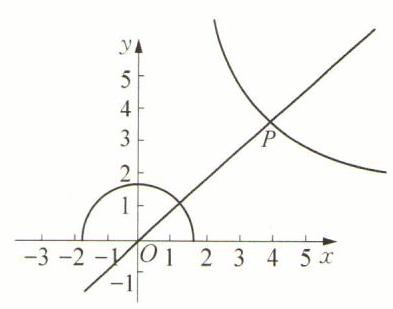
\includegraphics[max width=0.3\textwidth]{images/bo_d29ci7n7aajc738p8c80_18_1101_593_393_309_0.jpg}
\end{center}
\hspace*{3em} 

第 7 题图

8.【答案】-4

【解析】若 $a > 0$ ,由于 $a{x}^{2} + {bx} \geq  0$ ,即 $x\left( {{ax} + b}\right)  \geq  0$ ,所以对于正数 $b$ ,解得 $x \geq  0$ 或 $x \leq   - \dfrac{b}{a}$ ,所以 $f\left( x\right)$ 的定义域为 $D = \left( {-\infty , - \dfrac{b}{a}}\right\rbrack   \cup  \lbrack 0, + \infty )$ ,但 $f\left( x\right)$ 的值域 $A \subseteq  \lbrack 0$ , $+ \infty )$ ,故 $D \neq  A$ ,不符合要求.

若 $a < 0$ ,由于 $a{x}^{2} + {bx} \geq  0$ ,即 $x\left( {{ax} + b}\right)  \geq  0$ ,对于正数 $b$ ,解得 $0 \leq  x \leq   - \dfrac{b}{a}$ ,所以 $f\left( x\right)$ 的定义域为 $D = \left\lbrack  {0, - \dfrac{b}{a}}\right\rbrack$ . 由于此时函数 $f{\left( x\right) }_{\max } = f\left( {-\dfrac{b}{2a}}\right)  = \sqrt{a \times  {\left( \dfrac{b}{2a}\right) }^{2} + b \times  \left( {-\dfrac{b}{2a}}\right) } =$  $\sqrt{\dfrac{-{b}^{2}}{4a}} = \dfrac{b}{2}\sqrt{\dfrac{1}{-a}}.$

故函数的值域 $A = \left\lbrack  {0,\dfrac{b}{2}\sqrt{\dfrac{1}{-a}}}\right\rbrack$ ,由题意,有 $- \dfrac{b}{a} = \dfrac{b}{2}\sqrt{\dfrac{1}{-a}}$ ,由于 $b > 0$ ,解得 $a =  - 4$ .

9.【答案】\{ $- 3,0,2\}$

【解析】 $f\left( x\right)  = \dfrac{{2}^{x + 1}}{{2}^{x} + 1} - 1 = \dfrac{2\left( {{2}^{x} + 1}\right)  - 2}{{2}^{x} + 1} - 1 = \dfrac{-2}{{2}^{x} + 1} + 1$ ,因为 $f\left( {-x}\right)  + f\left( x\right)  =$  $\left( {\dfrac{-2}{{2}^{-x} + 1} + 1}\right)  + \left( {\dfrac{-2}{{2}^{x} + 1} + 1}\right)  = \dfrac{-2 \cdot  {2}^{x}}{{2}^{x} + 1} + \dfrac{-2}{{2}^{x} + 1} + 2 = \dfrac{-2\left( {{2}^{x} + 1}\right) }{{2}^{x} + 1} + 2 = 0$ ,所以 $f\left( x\right)$ 为奇函数. 又因为当 $x < 0$ 时, $- 1 < f\left( x\right)  < 0$ ,当 $x > 0$ 时, $0 < f\left( x\right)  < 1$ ,所以当 $x > 0$ 时, $0 < f\left( x\right)  < 1, - 1 < f\left( {-x}\right)  < 0$ ,此时 $\left\lbrack  {f\left( x\right) }\right\rbrack   = 0,3\left\lbrack  {f\left( x\right) }\right\rbrack   = 0$ , $\left\lbrack  {f\left( {-x}\right) }\right\rbrack   =  - 1,2\left\lbrack  {f\left( {-x}\right) }\right\rbrack   =  - 2$ ,则 $3\left\lbrack  {f\left( x\right) }\right\rbrack   - 2\left\lbrack  {f\left( {-x}\right) }\right\rbrack   = 2$ ;

当 $x < 0$ 时, $- 1 < f\left( x\right)  < 0,0 < f\left( {-x}\right)  < 1$ ,此时 $\left\lbrack  {f\left( x\right) }\right\rbrack   =  - 1,3\left\lbrack  {f\left( x\right) }\right\rbrack   =  - 3$ , $\left\lbrack  {f\left( {-x}\right) }\right\rbrack   = 0,2\left\lbrack  {f\left( {-x}\right) }\right\rbrack   = 0$ ,则 $3\left\lbrack  {f\left( x\right) }\right\rbrack   - 2\left\lbrack  {f\left( {-x}\right) }\right\rbrack   =  - 3$ ; 当 $x = 0$ 时, $f\left( x\right)  = f\left( {-x}\right)  = 0$ ,此时 $\left\lbrack  {f\left( x\right) }\right\rbrack   = \left\lbrack  {f\left( {-x}\right) }\right\rbrack   = 0$ ,则 $3\left\lbrack  {f\left( x\right) }\right\rbrack   - 2\left\lbrack  {f\left( {-x}\right) }\right\rbrack   = 0$ . 综上所述, $3\left\lbrack  {f\left( x\right) }\right\rbrack   - 2\left\lbrack  {f\left( {-x}\right) }\right\rbrack$ 的值域为 $\{  - 3,0,2\}$ .

10.【答案】 $\dfrac{\sqrt{5} - 1}{2}$

【解析】令 $x = \dfrac{1}{x + 1}$ ,得 $x = \dfrac{\sqrt{5} - 1}{2}$ 或 $x = \dfrac{-\sqrt{5} - 1}{2}$ (舍去). 当 $x \geq  \dfrac{\sqrt{5} - 1}{2}$ 时, $\dfrac{1}{x + 1} \leq$  $\dfrac{1}{\dfrac{\sqrt{5} - 1}{2} + 1} = \dfrac{\sqrt{5} - 1}{2}$ ,故对任意 $x \geq  \dfrac{\sqrt{5} - 1}{2}$ ,都存在 ${x}_{0} \in  \left\lbrack  {0,\dfrac{\sqrt{5} - 1}{2}}\right\rbrack  ,\dfrac{1}{x + 1} = {x}_{0}$ ,故

$f\left( x\right)  = f\left( {x}_{0}\right)$ ,故 $A = \left\{  {y\left| {y = f\left( x\right) }\right. ,x \in  \left\lbrack  {0,\dfrac{\sqrt{5} - 1}{2}}\right\rbrack  }\right\}$ ; 而当 $0 \leq  x < \dfrac{\sqrt{5} - 1}{2}$ 时, $\dfrac{1}{x + 1} > \dfrac{1}{\dfrac{\sqrt{5} - 1}{2} + 1} = \dfrac{\sqrt{5} - 1}{2}$ . 故当 $A = \{ y \mid  y = f\left( x\right) ,x \in  \left\lbrack  {0,a}\right\rbrack  \}$ 时,参数 $a$ 的最小值为 $\dfrac{\sqrt{5} - 1}{2}$ .

\section*{06 函数中的恒成立与存在性问题}

1.【答案】 $\left( {-\infty ,\dfrac{9}{4}}\right\rbrack$

【解析】当 $x = 0$ 时, $y = 0$ ,此时恒成立；当 $x \in  (0,1\rbrack$ 时,要使 $y = a{x}^{3} + 3\left( {a - 1}\right) {x}^{2} - {6x} \leq$ 0 恒成立,通过分离参数 $a$ ,化简可得 $a \leq  \dfrac{3\left( {x + 2}\right) }{x\left( {x + 3}\right) }$ 恒成立,令 $g\left( x\right)  = \dfrac{3\left( {x + 2}\right) }{x\left( {x + 3}\right) }$ ,则 $a \leq$  $g{\left( x\right) }_{\min }$ ,变形得 $g\left( x\right)  = \dfrac{3\left( {x + 2}\right) }{x\left( {x + 3}\right) } = \dfrac{3}{\dfrac{x\left( {x + 3}\right) }{x + 2}} = \dfrac{3}{\left( {x + 2}\right)  - \dfrac{2}{x + 2} - 1}$ ,则 $g\left( x\right)$ 在 $(0,1\rbrack$ 时单调递减, $g{\left( x\right) }_{\min } = g\left( 1\right)  = \dfrac{9}{4}$ ,则 $a \leq  \dfrac{9}{4}$ .

2.【答案】B

【解析】因为函数 $f\left( x\right)  = \lg \dfrac{a}{{2}^{x} + 1}$ 为 “可拆分函数”,所以存在实数 ${x}_{0}$ ,使 $\lg \dfrac{a}{{2}^{{x}_{0} + 1} + 1} =$  $\lg \dfrac{a}{{2}^{{x}_{0}} + 1} + \lg \dfrac{a}{3} = \lg \dfrac{{a}^{2}}{3\left( {{2}^{{x}_{0}} + 1}\right) }$ 成立,所以方程 $\dfrac{a}{{2}^{{x}_{0} + 1} + 1} = \dfrac{{a}^{2}}{3\left( {{2}^{{x}_{0}} + 1}\right) }$ 在 ${x}_{0} \in  \mathbf{R}$ 上有解,即 $a = \dfrac{3\left( {{2}^{{x}_{0}} + 1}\right) }{{2}^{{x}_{0} + 1} + 1} = \dfrac{3}{2} + \dfrac{3}{2} \cdot  \dfrac{1}{{2}^{{x}_{0} + 1} + 1}$ 在 ${x}_{0} \in  \mathbf{R}$ 上有解. 因为 ${x}_{0} \in  \mathbf{R}$ ,所以 $\dfrac{1}{{2}^{{x}_{0} + 1} + 1} \in  \left( {0,1}\right)$ , 所以 $a \in  \left( {\dfrac{3}{2},3}\right)$ ,得 $a$ 的取值范围为 $\left( {\dfrac{3}{2},3}\right)$ .

3.【答案】 $\left\lbrack  {0,\dfrac{2}{3}}\right\rbrack$

【解析】首先研究函数的定义域,有 $\left\{  \begin{array}{l} x \geq   - 3, \\  {ax} + 2 \neq  0. \end{array}\right.$ ① 当 $a = 0$ 时, $f\left( x\right)  = \sqrt{x + 3} + \dfrac{1}{2}$ 定义域为 $\lbrack  - 3, + \infty )$ ,此时 $f\left( x\right)$ 的值域为 $\left\lbrack  {\dfrac{1}{2}, + \infty }\right)$ 满足值域为 $\left( {0, + \infty }\right)$ 的子集; ② 当 $a = \dfrac{2}{3}$ 时, $f\left( x\right)  = \sqrt{x + 3} + \dfrac{3}{{2x} + 6}$ 定义域为 $\left( {-3, + \infty }\right)$ ,则 $\sqrt{x + 3} \geq  0,\dfrac{3}{{2x} + 6} > 0$ ,所以 $f\left( x\right)  > 0$ ,满足值域为 $\left( {0, + \infty }\right)$ 的子集; ③ 当 $a < 0$ 时,在 $x$ 略大于 $- \dfrac{2}{a}$ 时,有 $f\left( x\right)$ 趋近于负无穷,不符合题意; ④ 当 $a > 0$ 且 $a \neq  \dfrac{2}{3}$ 时,因为 ${ax} + 2 \in  \lbrack  - {3a} + 2, + \infty )$ ,要使 $f\left( x\right)  = \sqrt{x + 3} + \dfrac{1}{{ax} + 2}$ 的值域为 $\left( {0, + \infty }\right)$ 的子集,所以需要 ${ax} + 2 > 0$ 在 $\lbrack  - 3, + \infty )$ 上恒成立,得 $\left\{  \begin{array}{l} a > 0, \\   - {3a} + 2 > 0, \end{array}\right.$ 解得 $0 < a < \dfrac{2}{3}$ .

综上可得: 实数 $a$ 的取值范围是 $\left\lbrack  {0,\dfrac{2}{3}}\right\rbrack$ .

4.【答案】 $a \geq  1$ 或 $a \leq   - 1$

【解析】由题知, $\left| {x + {a}^{2}}\right|  + \left| {x - {a}^{2}}\right|  =  - {x}^{2} + {2x} - 1 + 2{a}^{2}$ 有解 $\Rightarrow  \left| {x + {a}^{2}}\right|  + \left| {x - {a}^{2}}\right|  +$  ${\left( x - 1\right) }^{2} = 2{a}^{2}$ 有解.

因为 $f\left( x\right)  = \left| {x + {a}^{2}}\right|  + \left| {x - {a}^{2}}\right|  + {\left( x - 1\right) }^{2} \geq  2{a}^{2}$ 恒成立,当且仅当 $\left\{  \begin{array}{l}  - {a}^{2} \leq  x \leq  {a}^{2}, \\  x = 1 \end{array}\right.$ 时等号成立,故原等式要有解,必须达到取等条件,可解得 $a \geq  1$ 或 $a \leq   - 1$ .

5.【答案】 $\left( {-\infty , - \dfrac{3}{4}}\right\rbrack$

【解析】若对任意的 ${x}_{1},{x}_{2} \in  \{ x \mid  x \in  \mathbf{R},x >  - 2\}$ ,均有 $f\left( {x}_{1}\right)  \leq  g\left( {x}_{2}\right)$ ,则 $f{\left( x\right) }_{\max } \leq$  $g{\left( x\right) }_{\min }$ ,由于 $g\left( x\right)  = a \cdot  \lg \left( {x + 2}\right)  + \dfrac{x}{{x}^{2} + 1}\left( {a \in  \mathbf{R}}\right)$ ,因为 $h\left( x\right)  = \lg \left( {x + 2}\right)$ 值域为 $\mathbf{R}$ , 所以若 $a \neq  0,g\left( x\right)$ 无最小值,原不等式不可能成立,所以可得 $a = 0,g\left( x\right)  = \dfrac{x}{{x}^{2} + 1}\left( {a \in  }\right.$ R). 当 $x = 0$ 时, $\dfrac{x}{{x}^{2} + 1} = 0$ ; 当 $x \neq  0,\dfrac{x}{{x}^{2} + 1} = \dfrac{1}{x + \dfrac{1}{x}} \in  \left\lbrack  {-\dfrac{1}{2},0) \cup  \left( {0,\dfrac{1}{2}}\right\rbrack  }\right\rbrack$ ,所以 $g{\left( x\right) }_{\min } =  - \dfrac{1}{2}$ . 因为 $y =  - \dfrac{1}{2} + {\log }_{\dfrac{1}{2}}x$ 为减函数,所以当 $x > 1$ 时, $f\left( x\right)  =  - \dfrac{1}{2} + {\log }_{\dfrac{1}{2}}x$  $<  - \dfrac{1}{2}$ ; 当 $- 2 < x \leq  1$ 时, $f\left( x\right)  =  - {x}^{2} + x + k =  - {\left( x - \dfrac{1}{2}\right) }^{2} + \dfrac{1}{4} + k \leq  \dfrac{1}{4} + k$ . 所以 $\dfrac{1}{4} + k \leq   - \dfrac{1}{2}$ ,解得 $k \leq   - \dfrac{3}{4}$ ,即实数 $k$ 的取值范围是 $\left( {-\infty , - \dfrac{3}{4}}\right\rbrack$ .

6.【答案】A

【解析】因为 $x \in  \left\lbrack  {0,3}\right\rbrack$ ,所以 ${x}^{2} + 1 \in  \left\lbrack  {1,{10}}\right\rbrack  ,\lg \left( {{x}^{2} + 1}\right)  \in  \left\lbrack  {0,1}\right\rbrack$ ,即 $f\left( x\right)  \in  \left\lbrack  {0,1}\right\rbrack$ . 由 $x \in  \left\lbrack  {1,2}\right\rbrack$ ,则 ${\left( \dfrac{1}{2}\right) }^{x} - m \in  \left\lbrack  {\dfrac{1}{4} - m,\dfrac{1}{2} - m}\right\rbrack$ ,即 $g\left( x\right)  \in  \left\lbrack  {\dfrac{1}{4} - m,\dfrac{1}{2} - m}\right\rbrack$ . 因为对于任意 ${x}_{1} \in  \left\lbrack  {0,3}\right\rbrack$ ,存在 ${x}_{2} \in  \left\lbrack  {1,2}\right\rbrack$ ,使得 $f\left( {x}_{1}\right)  \leq  g\left( {x}_{2}\right)$ ,所以 $f{\left( {x}_{1}\right) }_{\max } \leq  g{\left( {x}_{2}\right) }_{\max }$ , 则 $\dfrac{1}{2} - m \geq  1$ ,解得 $m \leq   - \dfrac{1}{2}$ ,即 $m \in  \left( {-\infty , - \dfrac{1}{2}}\right\rbrack$ .

7.【答案】 ${C}$

【解析】易知 $f\left( x\right)$ 的值域为 $\left\lbrack  {1,3}\right\rbrack$ ,记为 $A = \left\lbrack  {1,3}\right\rbrack$ ,当 $a > 0$ 时, $g\left( x\right)$ 的值域为 $\lbrack  - a - 1$ , $a - 1\rbrack$ ,记为 $B = \left\lbrack  {-a - 1,a - 1}\right\rbrack$ ;当 $a < 0$ 时, $g\left( x\right)$ 的值域为 $\left\lbrack  {a - 1, - a - 1}\right\rbrack$ ,记为 $C =$  $\left\lbrack  {a - 1, - a - 1}\right\rbrack$ . 当 $a > 0$ 时,由题意可知 $A = \left\lbrack  {1,3}\right\rbrack$ 是 $B = \left\lbrack  {-a - 1,a - 1}\right\rbrack$ 的子集,所以 $\left\{  \begin{array}{l}  - a - 1 \leq  1, \\  a - 1 \geq  3, \end{array}\right.$ 得 $a \geq  4$ ; 当 $a < 0$ 时,由题意可知 $A = \left\lbrack  {1,3}\right\rbrack$ 是 $C = \left\lbrack  {a - 1, - a - 1}\right\rbrack$ 的子集,所以 $\left\{  \begin{array}{l} a - 1 \leq  1, \\   - a - 1 \geq  3, \end{array}\right.$ 得 $a \leq   - 4$ . 综上, $a \geq  4$ 或 $a \leq   - 4$ .

8.【答案】 $\left\lbrack  {\dfrac{5}{4},\dfrac{4}{3}}\right\rbrack$

【解析】由 $f\left( {x}_{1}\right) f\left( {x}_{2}\right)  = g\left( {x}_{1}\right) g\left( {x}_{2}\right)$ 可得 ${x}_{1}{x}_{2} = \left( {a{x}_{1}^{2} - {x}_{1}}\right) \left( {a{x}_{2}^{2} - {x}_{2}}\right)$ ,化简得 ${a}^{2}{x}_{1}^{2}{x}_{2}^{2} - a{x}_{1}^{2}{x}_{2} - a{x}_{1}{x}_{2}^{2} = 0$ . 因为 $a > 0,{x}_{1} \in  \left\lbrack  {1,3}\right\rbrack  ,{x}_{2} \in  \left\lbrack  {1,4}\right\rbrack$ ,所以 $a{x}_{1}{x}_{2} - {x}_{1} -$  ${x}_{2} = 0$ ,即 $a = \dfrac{{x}_{1} + {x}_{2}}{{x}_{1}{x}_{2}} = \dfrac{1}{{x}_{1}} + \dfrac{1}{{x}_{2}}$ ,所以 $a - \dfrac{1}{{x}_{2}} = \dfrac{1}{{x}_{1}}$ . 因为 $\dfrac{1}{{x}_{1}} \in  \left\lbrack  {\dfrac{1}{3},1}\right\rbrack$ ,且 $a - \dfrac{1}{{x}_{2}} \in$

$\left\lbrack  {a - 1,a - \dfrac{1}{4}}\right\rbrack$ ,由对任意的 ${x}_{1} \in  \left\lbrack  {1,3}\right\rbrack$ ,总存在 ${x}_{2} \in  \left\lbrack  {1,4}\right\rbrack$ ,有 $a - \dfrac{1}{{x}_{2}} = \dfrac{1}{{x}_{1}}$ 成立,所以 $\left\lbrack  {\dfrac{1}{3},1}\right\rbrack   \subseteq  \left\lbrack  {a - 1,a - \dfrac{1}{4}}\right\rbrack$ ,得 $\left\{  \begin{array}{l} \dfrac{1}{3} \geq  a - 1, \\  1 \leq  a - \dfrac{1}{4}, \end{array}\right.$ 解得 $\dfrac{5}{4} \leq  a \leq  \dfrac{4}{3}$ ,即实数 $a$ 的取值范围是 $\left\lbrack  {\dfrac{5}{4},\dfrac{4}{3}}\right\rbrack$

9.【答案】( $- \infty ,\sqrt{{e}}$ )

【解析】由题意可得: 存在 $x < 0$ ,使得 $f\left( x\right)  = g\left( {-x}\right)$ 成立,即 ${x}^{2} + {{e}}^{x} - \dfrac{1}{2} = {\left( -x\right) }^{2} +$  $\ln \left( {-x + a}\right)$ 有负解. 所以 ${{e}}^{x} - \dfrac{1}{2} = \ln \left( {-x + a}\right)  \Rightarrow   - x + a = {{e}}^{{{e}}^{x} - \dfrac{1}{2}} \Rightarrow  a = {{e}}^{{{e}}^{x} - \dfrac{1}{2}} + x$ 有负解. 令 $m\left( x\right)  = {{e}}^{{{e}}^{x} - \dfrac{1}{2}} + x\left( {x < 0}\right)$ ,易得 $m\left( x\right)$ 在 $\left( {-\infty ,0}\right)$ 上单调递增,当 $x \rightarrow   - \infty$ 时 $m\left( x\right)  \rightarrow$  $- \infty ,m\left( 0\right)  = \sqrt{{e}}$ ,所以 $m\left( x\right)$ 的值域为 $\left( {-\infty ,\sqrt{{e}}}\right)$ ,所以实数 $a$ 的取值范围是 $\left( {-\infty ,\sqrt{{e}}}\right.$ .

10.【答案】 $\dfrac{\sqrt{6} - 2}{4}$

【解析】由题意知 $3{x}^{3} + \left( {{2a} - 1}\right) x + a\sqrt{2 - 2{x}^{2}} \geq  0,x \in  \left( {0,\dfrac{\sqrt{3}}{3}}\right) \cdots \left( *\right)$ 恒成立,且等号能取到.

由 $x\left( {3{x}^{2} - 1}\right)  + a\left( {{2x} + \sqrt{2 - 2{x}^{2}}}\right)  \geq  0$ ,得 $a \geq  \dfrac{1 - 3{x}^{2}}{2 + \sqrt{\dfrac{2}{{x}^{2}} - 2}}$ 恒成立.

令 $t = \sqrt{\dfrac{2}{{x}^{2}} - 2}\left( {t > 2}\right)$ ,则 ${x}^{2} = \dfrac{2}{{t}^{2} + 2}$ ,得 $a \geq  \dfrac{1 - 3 \cdot  \dfrac{2}{{t}^{2} + 2}}{t + 2} = \dfrac{t - 2}{{t}^{2} + 2}$ .

令 $g\left( t\right)  = \dfrac{t - 2}{{t}^{2} + 2} = \dfrac{t - 2}{{\left( t - 2\right) }^{2} + 4\left( {t - 2}\right)  + 6} = \dfrac{1}{\left( {t - 2}\right)  + \dfrac{6}{t - 2} + 4} \leq  \dfrac{1}{2\sqrt{6} + 4} = \dfrac{\sqrt{6} - 2}{4}$ ,当且

仅当 $t = 2 + \sqrt{6}$ 时等号成立. 所以 $a \geq  \dfrac{\sqrt{6} - 2}{4}$ .

因为 (*) 恰好取到等号,所以 $a = \dfrac{\sqrt{6} - 2}{4}$ .

\section*{07 函数的递推}

1.【答案】B

【解析】由题应有 $f\left( {93}\right)  - f\left( {91}\right)  = {91},f\left( {91}\right)  - f\left( {89}\right)  = {89},\cdots ,f\left( 3\right)  - f\left( 1\right)  = 1$ ,累加可得 $f\left( {93}\right)  - f\left( 1\right)  = {91} + {89} + \cdots  + 1 = {2116}$ ,又 $f\left( 1\right)  = 1 - 8 =  - 7$ ,得 $f\left( {93}\right)  = {2109}$ .

2.【答案】 $\left\lbrack  {\dfrac{1}{4},{16}}\right\rbrack$

【解析】由题可得 $f\left( {x + 1}\right)  = {2}^{x + 1} \cdot  g\left( {x + 1}\right)  = {2}^{x + 1} \cdot  g\left( x\right)  = {2f}\left( x\right)$ . 于是当 $x \in  \left\lbrack  {1,2}\right\rbrack$ 时, $y = f\left( x\right)$ 的值域为 $\left\lbrack  {\dfrac{1}{2},2}\right\rbrack$ ; 当 $x \in  \left\lbrack  {0,1}\right\rbrack$ 时, $y = f\left( x\right)$ 的值域为 $\left\lbrack  {\dfrac{1}{4},1}\right\rbrack$ ; 当 $x \in  \lbrack 3$ , 4]时, $y = f\left( x\right)$ 的值域为 $\left\lbrack  {2,8}\right\rbrack  ;x \in  \left\lbrack  {4,5}\right\rbrack$ 时, $y = f\left( x\right)$ 的值域为 $\left\lbrack  {4,{16}}\right\rbrack$ . 综上,函数 $y =$  $f\left( x\right) ,x \in  \left\lbrack  {0,5}\right\rbrack$ 的值域为 $\left\lbrack  {\dfrac{1}{4},{16}}\right\rbrack$ .

3.【答案】B

【解析】令 $y = 1$ 得 $f\left( x\right)  = f\left( {x + 1}\right)  + f\left( {x - 1}\right)$ ,即有 $f\left( {x + 1}\right)  = f\left( {x + 2}\right)  + f\left( x\right)$ ,两式相加可得 $f\left( {x + 2}\right)  =  - f\left( {x - 1}\right)$ ,即有 $f\left( {x + 5}\right)  =  - f\left( {x + 2}\right)$ ,得 $f\left( {x + 5}\right)  = f\left( {x - 1}\right)$ , 即有函数周期为 6,故 $f\left( {2015}\right)  = f\left( {-1}\right)  =  - f\left( 2\right)$ . 令 $x = 1,y = 0$ 得 $f\left( 0\right)  = \dfrac{1}{2}$ ,令 $x = 1$ , $y = 1$ 得 $\dfrac{1}{4} = f\left( 2\right)  + \dfrac{1}{2}$ ,得 $f\left( 2\right)  =  - \dfrac{1}{4}$ ,得 $f\left( {2015}\right)  = \dfrac{1}{4}$ .

4.【答案】 3535

【解析】由 $f\left( {n + 4}\right)  - f\left( n\right)  \leq  2\left( {n + 1}\right)$ ,得 $f\left( {n + 8}\right)  - f\left( {n + 4}\right)  \leq  2\left( {n + 5}\right) ,f\left( {n + {12}}\right)  -$  $f\left( {n + 8}\right)  \leq  2\left( {n + 9}\right)$ ,三式相加可得 $f\left( {n + {12}}\right)  - f\left( n\right)  \leq  {2n} + 2 + {2n} + {10} + {2n} + {18} =$  $6\left( {n + 5}\right)$ (取等条件为前三个不等式都取等号),又 $f\left( {n + {12}}\right)  - f\left( n\right)  \geq  6\left( {n + 5}\right)$ ,所以有 $f\left( {n + {12}}\right)  - f\left( n\right)  = 6\left( {n + 5}\right)$ ,且 $f\left( {n + 4}\right)  - f\left( n\right)  = 2\left( {n + 1}\right)$ .

于是 $f\left( {2023}\right)  - f\left( {2019}\right)  = 2\left( {{2019} + 1}\right) ,f\left( {2019}\right)  - f\left( {2015}\right)  = 2\left( {{2015} + 1}\right)$ ,以此类推,得 $f\left( 3\right)  - f\left( {-1}\right)  = 2\left( {-1 + 1}\right)$ ,共 506 个等式,累加得 $f\left( {2023}\right)  - f\left( {-1}\right)  = 2({2019} +$ 2015 + … + 3-1 + 1 × 506),即有 $f\left( {2023}\right)  =  - {505} + 2 \times  \left( {\dfrac{{2019} - 1}{2} \times  {506} + {506}}\right)  =$ 1021615,所以 $\dfrac{f\left( {2023}\right) }{289} = {3535}$ .

5.【答案】A

【解析】当 $a > 0$ 时, $f\left( x\right)$ 在 $\left\lbrack  {0,1}\right\rbrack$ 上的值域为 $\left\lbrack  {\dfrac{a}{3} + 1,\dfrac{a}{2} + 1}\right\rbrack$ ,在(1,2)上的值域为 $\left( {\dfrac{a}{3} + 1,\dfrac{2a}{3} + 1}\right)$ ,故 $f\left( x\right)$ 在 $\lbrack 0,2)$ 上的值域为 $\left\lbrack  {\dfrac{a}{3} + 1,\dfrac{2a}{3} + 1}\right)$ ,可得 $f\left( x\right)$ 在 $\lbrack 2,4)$ 上的

值域为 $\left\lbrack  {\dfrac{4a}{3} + 1,\dfrac{5a}{3} + 1}\right)$ ,进而得 $f\left( x\right)$ 在 $\lbrack 8,{10})$ 上的值域为 $\left\lbrack  {\dfrac{13a}{3} + 1,\dfrac{14a}{3} + 1}\right)$ . 由题应有

$\left\{  \begin{array}{l} b + 3 \geq  \dfrac{14a}{3} + 1, \\  b \leq  \dfrac{a}{3} + 1, \end{array}\right.$ 该不等式组关于 $b$ 有解,得 $\dfrac{14a}{3} + 1 \leq  \dfrac{a}{3} + 1 + 3$ ,解得 $a \leq  \dfrac{9}{13}$ ; 当 $a < 0$ 时,

易得 $f\left( x\right)$ 在 $\lbrack 0,2)$ 上的值域为 $\left\lbrack  {\dfrac{2a}{3} + 1,\dfrac{a}{3} + 1}\right)$ ,可进一步得 $f\left( x\right)$ 在 $\lbrack 8,{10})$ 上的值域为 $\left\lbrack  {\dfrac{14a}{3} + 1,\dfrac{13a}{3} + 1}\right)$ ,得不等式组 $\left\{  \begin{array}{l} b + 3 \geq  \dfrac{a}{3} + 1, \\  b \leq  \dfrac{14a}{3} + 1 \end{array}\right.$ 关于 $b$ 有解,得 $a \geq   - \dfrac{9}{13}$ . 所以,满足条件的 $a$ 的范围是 $- \dfrac{9}{13} \leq  a \leq  \dfrac{9}{13}$ ,显然 $a = \dfrac{7}{12}$ 符合.

6.【答案】 $1 + 2\sqrt{2}$

【解析】由 $f\left( {x + 1}\right)  - 1 = \sqrt{{f}^{2}\left( x\right)  - {2f}\left( x\right)  + 1 + 4}\left( {x \geq  0}\right)$ ,得 $f\left( n\right)  \geq  1\left( {n \geq  1}\right)$ 且 ${\left( f\left( n\right)  - 1\right) }^{2} = {\left( f\left( n - 1\right)  - 1\right) }^{2} + 4$ ,即 $\dfrac{1}{4}{\left( f\left( n\right)  - 1\right) }^{2} = \dfrac{1}{4}{\left( f\left( n - 1\right)  - 1\right) }^{2} + 1$ ,由题 ${a}_{n} =$  $\dfrac{1}{4}{\left( f\left( n\right)  - 1\right) }^{2}$ ,所以 $\left\{  {a}_{n}\right\}$ 是公差为 1 的等差数列,易得 ${a}_{1} = 2$ ,代入解得 $f\left( 1\right)  = 1 + 2\sqrt{2}$ 或 $1 - 2\sqrt{2}$ (舍).

7.【答案】1008

【解析】令 $y = 0$ ,得 $f\left( 0\right)  = 0$ ,令 $x = 0,y = 1$ ,得 $f\left( 1\right)  = 0 + 2{f}^{2}\left( 1\right)$ ,又 $f\left( 1\right)  \neq  0$ ,得 $f\left( 1\right)  =$  $\dfrac{1}{2}$ . 令 $y = 1$ 得 $f\left( {x + 1}\right)  = f\left( x\right)  + \dfrac{1}{2}$ ,故 $f\left( {2016}\right)  = f\left( {2015}\right)  + \dfrac{1}{2} = f\left( {2014}\right)  + 2 \times  \dfrac{1}{2} =$  $f\left( {2013}\right)  + 3 \times  \dfrac{1}{2} = \cdots  = f\left( 1\right)  + {2015} \times  \dfrac{1}{2} = {1008}.$

\section*{08 函数的单调性}

1.【答案】 ${D}$

【解析】① 设 $t = \sqrt{x},x \in  \left( {0,1}\right)$ 单调递增, $y =  - {t}^{2} + {2t},t \in  \left( {0,1}\right)$ 单调递增,故 $f\left( x\right)$ 在(0,1)上单调递增, $\dfrac{f\left( x\right) }{x} = \dfrac{2}{\sqrt{x}} - 1,x \in  \left( {0,1}\right)$ 单调递减,故函数 $f\left( x\right)$ 是(0,1)上的 “ $H$ 函数”.

② $g\left( x\right)  = \dfrac{2}{\dfrac{1}{x} - x},x \in  \left( {0,1}\right)$ 单调递增, $\dfrac{g\left( x\right) }{x} = \dfrac{2}{1 - {x}^{2}},x \in  \left( {0,1}\right)$ 单调递增,故函数

$g\left( x\right)$ 不是(0,1)上的 “ $H$ 函数”.

所以, ① 真 ② 假.

2.【答案】A

【解析】在 ${f}_{1}\left( x\right)$ 中,任意 $a > 0$ ,由单调递增可得 ${f}_{1}\left( {x + a}\right)  > {f}_{1}\left( x\right)$ ,又 ${f}_{1}\left( a\right)  \leq  0$ ,所以存在 $a > 0$ ,使得 ${f}_{1}\left( {x + a}\right)  > {f}_{1}\left( x\right)  + {f}_{1}\left( a\right)$ ,故 ${f}_{1}\left( x\right)$ 具有 “ $P$ 性质”; 在 ${f}_{2}\left( x\right)$ 中,设 $a = {x}_{0} < 0$ ,由单调递减可得 ${f}_{2}\left( {x + a}\right)  > {f}_{2}\left( x\right)$ ,又 ${f}_{2}\left( a\right)  = 0$ ,所以存在 $a < 0$ ,使得 ${f}_{2}\left( {x + a}\right)  > {f}_{2}\left( x\right)  + {f}_{2}\left( a\right)$ ,故 ${f}_{2}\left( x\right)$ 具有“ $P$ 性质”.

3.【答案】B

【解析】对任意 ${x}_{1} < {x}_{2}$ ,都有 $\dfrac{f\left( {x}_{1}\right)  - f\left( {x}_{2}\right) }{{x}_{1} - {x}_{2}} > a$ ,可得 $f\left( {x}_{1}\right)  - a{x}_{1} < f\left( {x}_{2}\right)  - a{x}_{2}$ ,即函数 $y = f\left( x\right)  - {ax}$ 严格单调递增. 设 $h\left( {x + a}\right)  = f\left( {a + x}\right)  - {ax} = f\left( {a + x}\right)  - a\left( {x + a}\right)  +$  ${a}^{2}$ ,则有 $h\left( x\right)  = f\left( x\right)  - {ax} + {a}^{2}$ ,故 $h\left( x\right)$ 在 $\mathbf{R}$ 上严格单调递增,又 $h\left( 0\right)  = f\left( 0\right)  + {a}^{2} = 0$ , 所以对任意常数 $a$ ,方程 $f\left( x\right)  = a\left( {x - a}\right)$ 有且仅有 1 解,即 $f\left( {x + a}\right)  = {ax}$ 有且仅有一解.

4.【答案】(1, $2\sqrt{2}$ )

【解析】由题意, $f\left( x\right)$ 在 $\left( {-\infty ,\dfrac{a}{2}}\right\rbrack$ 上单调递减. 易知 $f\left( x\right)$ 为复合函数,可分解为 $\left\{  \begin{array}{l} y = {\log }_{a}u, \\  u = {x}^{2} - {ax} + 2. \end{array}\right.$ 因为内函数 $u = {x}^{2} - {ax} + 2$ 在 $x \in  \left( {-\infty ,\dfrac{a}{2}}\right\rbrack$ 时严格单调递减,根据复合函数单调性的判断方法,外函数需要单调递增,所以 $a > 1$ . 因为 $f\left( x\right)$ 在 $\left( {-\infty ,\dfrac{a}{2}}\right\rbrack$ 上单调递减,故 $x \in  \left( {-\infty ,\dfrac{a}{2}}\right\rbrack$ 时, $u = {x}^{2} - {ax} + 2 > 0$ 恒成立,故 ${\left( \dfrac{a}{2}\right) }^{2} - a \cdot  \dfrac{a}{2} + 2 > 0$ ,解得 $a \in  \left( {1,2\sqrt{2}}\right)$ .

5.【答案】 $\left\lbrack  {\dfrac{1}{2},2}\right\rbrack$

【解析】因为任意函数图象关于 $y$ 轴对称后,其单调性相反变化. 若函数 $y = f\left( x\right)$ 和 $y =$  $g\left( x\right)$ 在区间 $\left\lbrack  {a,b}\right\rbrack$ 上同时递增 (递减),即 $y = g\left( x\right)$ 在区间 $\left\lbrack  {a,b}\right\rbrack$ 上递增 (递减),则 $y =$  $g\left( x\right)$ 关于 $y$ 轴对称的函数 $y = f\left( x\right)$ 在区间 $\left\lbrack  {-b, - a}\right\rbrack$ 上单调递减 (递增),即 $y = f\left( x\right)$ 在区间 $\left\lbrack  {a,b}\right\rbrack$ 和区间 $\left\lbrack  {-b, - a}\right\rbrack$ 上单调性相反. 所以若区间 $\left\lbrack  {1,2}\right\rbrack$ 为函数 $y = \left| {{2}^{x} - t}\right|$ 的“不

动区间”,则 $y = f\left( x\right)$ 在区间 $\left\lbrack  {1,2}\right\rbrack$ 和区间 $\left\lbrack  {-2, - 1}\right\rbrack$ 上的单调性要相反. 而 $y = {2}^{x} - t$ 为严格单调递增函数,要使 $f\left( x\right)  = \left| {{2}^{x} - t}\right|$ 在区间 $\left\lbrack  {1,2}\right\rbrack$ 和区间 $\left\lbrack  {-2, - 1}\right\rbrack$ 上的单调性相反,只需 $y = {2}^{x} - t$ 在区间 $\left\lbrack  {1,2}\right\rbrack$ 和区间 $\left\lbrack  {-2, - 1}\right\rbrack$ 内的符号相反即可 (在 $x$ 轴下方的图象翻折到 $x$ 轴上方时,单调性也会相反变化).

欲使 $y = h\left( x\right)  = {2}^{x} - t$ 在区间 $\left\lbrack  {1,2}\right\rbrack$ 和区间 $\left\lbrack  {-2, - 1}\right\rbrack$ 内的符号相反,故 $h\left( {-1}\right) h\left( 1\right)  \leq$ 0(因为 $h\left( x\right)  = {2}^{x} - t$ 在 $\mathbf{R}$ 上严格单调递增, $h\left( {-1}\right) h\left( 1\right)  \leq  0$ 时,函数在区间 $\left\lbrack  {1,2}\right\rbrack$ 和区间 $\left\lbrack  {-2, - 1}\right\rbrack$ 内的符号必相反),解得 $t \in  \left\lbrack  {\dfrac{1}{2},2}\right\rbrack$ .

6.【答案】D

【解析】假设 ① 为真命题,那么当 $m = n$ 时,有 $f\left( {x}_{1}\right)  - f\left( {x}_{2}\right)  = g\left( {x}_{1}\right)  - g\left( {x}_{2}\right)$ ,即有 $h\left( x\right)  = f\left( x\right)  - g\left( x\right)  = {2}^{x} - {x}^{2} - {ax}$ 对任意的 $a$ ,都存在不相等的实数 ${x}_{1}\text{ 、 }{x}_{2}$ ,使得 $h\left( {x}_{1}\right)  = h\left( {x}_{2}\right)$ ,即对任意 $a,h\left( x\right)$ 不单调,同理对任意 $a$ 有 $\varphi \left( x\right)  = f\left( x\right)  + g\left( x\right)  = {2}^{x} +$  ${x}^{2} + {ax}$ 不单调. ${h}^{\prime }\left( x\right)  = {2}^{x}\ln 2 - {2x} - a,{h}^{\prime \prime }\left( x\right)  = {2}^{x}{\ln }^{2}2 - 2$ ,令 ${h}^{\prime \prime }\left( {x}_{0}\right)  = 0$ ,解得 ${x}_{0} =$  $\ln \dfrac{2}{{\ln }^{2}2}$ ,易得 ${h}^{\prime \prime }\left( x\right)$ 在 ${x}_{0}$ 左侧为负,右侧为正,故 ${h}^{\prime }\left( x\right)$ 在 ${x}_{0}$ 左侧严格递减,右侧严格递增. 所以,当 $a < {2}^{{x}_{0}}\ln 2 - 2{x}_{0}$ 时, ${h}^{\prime }\left( x\right)  \geq  {h}^{\prime }\left( {x}_{0}\right)$ ,即存在 $a$ ,使得 $h\left( x\right)$ 单调,故① 为假命题. 由 $\varphi \left( x\right)  = {2}^{x} + {x}^{2} + {ax},{\varphi }^{\prime }\left( x\right)  = {2}^{x}\ln 2 + {2x} + a$ ,易得 ${\varphi }^{\prime }\left( x\right)$ 严格递增,值域为 $\mathbf{R}$ ,所以对任意 $a,{\varphi }^{\prime }\left( x\right)  = 0$ 一定有解,设为 ${x}_{0}$ ,那么 $\varphi \left( x\right)$ 在 $\left( {-\infty ,{x}_{0}}\right)$ 严格递减,在 $\left( {x}_{0}\right.$ , 十∞)严格递增,故 ② 为真命题.

7.【答案】C

【解析】由题易得 $f\left( x\right)  = f\left( {-x}\right)$ ,则有 $f\left( x\right)$ 为偶函数,所以 $f\left( x\right)$ 在 $\left( {0, + \infty }\right)$ 上有四个单调区间,画图可得 $y = {x}^{2} + \left( {{3m} + 5}\right) x + 1$ 必须满足对称轴大于 0,且有两个不同的实根,

即 $\left\{  \begin{array}{l}  - \dfrac{{3m} + 5}{2} > 0, \\  \Delta  = {\left( 3m + 5\right) }^{2} - 4 > 0, \end{array}\right.$ 解得 $m <  - \dfrac{7}{3}$ .

\section*{09 函数的奇偶性和单调性}

1.【答案】 $a \leq   - \dfrac{8}{7}$

【解析】 $f\left( x\right)$ 是奇函数,当 $x < 0$ 时, $f\left( x\right)  \leq  7 - 6\left| a\right|$ ,易得当 $x > 0$ 时, $f\left( x\right)  \geq  6\left| a\right|  -$ 7,且有 $f\left( 0\right)  = 0$ ,所以 $\left\{  \begin{array}{l} 6\left| a\right|  - 7 \geq  a + 1, \\  0 \geq  a + 1, \end{array}\right.$ 解得 $a \leq   - \dfrac{8}{7}$ .

2.【答案】A

【解析】① 错误. 反例:当 $f\left( x\right)  = x,g\left( x\right)  = 0$ 时, $h\left( x\right)$ 不是奇函数.

② 错误. 反例:当 $f\left( x\right)  = \left\{  {\begin{array}{ll} x, & x \leq  0, \\  0, & x > 0, \end{array}g\left( x\right)  = \left\{  \begin{array}{ll} 0, & x \leq  0, \\   - x, & x > 0 \end{array}\right. }\right.$ 时, $h\left( x\right)  = 0$ 是奇函数.

③ 错误. 反例:当 $f\left( x\right)  = x,g\left( x\right)  =  - x$ 时, $f\left( x\right)$ 与 $g\left( x\right)$ 均为奇函数, $h\left( x\right)  = \left| x\right|$ 为偶函数.

三个论断均错误.

3.【答案】A

【解析】不妨设 $0 < {x}_{1} < {x}_{2}$ ,可得 ${x}_{2}f\left( {x}_{1}\right)  - {x}_{1}f\left( {x}_{2}\right)  > 0$ ,化简得 $\dfrac{f\left( {x}_{1}\right) }{{x}_{1}} > \dfrac{f\left( {x}_{2}\right) }{{x}_{2}}$ ,即 $g\left( x\right)  = \dfrac{f\left( x\right) }{x}$ 在 $\left( {0, + \infty }\right)$ 上严格递减. $g\left( {-x}\right)  = \dfrac{f\left( {-x}\right) }{-x} = \dfrac{-f\left( x\right) }{-x} = \dfrac{f\left( x\right) }{x} = g\left( x\right)$ ,故 $g\left( x\right)$ 为偶函数.

4.【答案】6

【解析】对 $g\left( x\right)$ ,令 $m = n = 0$ ,解得 $g\left( 0\right)  = 3$ . 令 $m = x,n =  - x$ ,得 $g\left( 0\right)  = g\left( x\right)  +$  $g\left( {-x}\right)  - 3 = 3$ ,即有 $g\left( x\right)$ 关于(0,3)对称. 又 $y = \dfrac{x\sqrt{1 - {x}^{2}}}{{x}^{2} + 1}$ 为奇函数,于是 $f\left( x\right)$ 关于 (0,3) 对称,所以 $p + q = 6$ .

5.【答案】(一3 , -1 ]

【解析】解法一: 设 $h\left( x\right)  = f\left( x\right)  + g\left( x\right) ,\varphi \left( x\right)  = f\left( x\right)  - g\left( x\right) ,h\left( {-x}\right)  = f\left( {-x}\right)  +$  $g\left( {-x}\right)  =  - f\left( x\right)  + g\left( x\right)$ ,所以 $\varphi \left( x\right)  =  - h\left( {-x}\right)$ . 得 $\varphi \left( x\right)$ 和 $h\left( x\right)$ 图象关于原点对称, 所以 $\varphi \left( x\right)$ 值域为 $( - 3, - 1\rbrack$ .

解法二: 因为 $f\left( x\right)  + g\left( x\right)$ 的值域为 $\lbrack 1,3)$ ,故 $y = f\left( {-x}\right)  + g\left( {-x}\right)$ 的值域也为 $\lbrack 1,3)$ . 又因为 $f\left( x\right)$ 是奇函数, $g\left( x\right)$ 是偶函数,故 $y = f\left( {-x}\right)  + g\left( {-x}\right)  =  - f\left( x\right)  + g\left( x\right)$ ,故 $f\left( x\right)  - g\left( x\right)  =  - \left\lbrack  {-f\left( x\right)  + g\left( x\right) }\right\rbrack$ ,因此 $f\left( x\right)  - g\left( x\right)$ 的值域为 $( - 3, - 1\rbrack$ .

\section*{10 函数的周期性和图象的对称性}

1.【答案】1009 或 1010

【解析】方程 $\dfrac{1}{1 - x} - 2\sin {\pi x} = 0 \Leftrightarrow  \dfrac{1}{1 - x} = 2\sin {\pi x}$ . 令函数 $f\left( x\right)  = \dfrac{1}{1 - x},g\left( x\right)  = 2\sin {\pi x}$ , 函数 $f\left( x\right)  = \dfrac{1}{1 - x}$ 图象关于点(1,0)对称,函数 $g\left( x\right)  = 2\sin {\pi x}$ 的图象也关于点(1,0)对

称,其图象如图所示. 因为区间 $\lbrack  - m - 1,m +$ 3] $\left( {m \in  \mathbf{Z}}\right)$ 关于 1 对称,所以函数 $f\left( x\right) ,g\left( x\right)$ 在 $\left\lbrack  {-m - 1,m + 3}\right\rbrack  \left( {m \in  \mathbf{Z}}\right)$ 的交点成对出现, 它们关于点 (1,0) 对称, 因此两函数图象在 $\left\lbrack  {-m - 1,m + 3}\right\rbrack  \left( {m \in  \mathbf{Z}}\right)$ 上有 1012 对关于点 (1,0) 对称的交点,则有 $m + 3 = {1012}$ 或 $m +$  $3 = {1013}$ ,解得 $m = {1009}$ 或 $m = {1010}$ .

\begin{center}
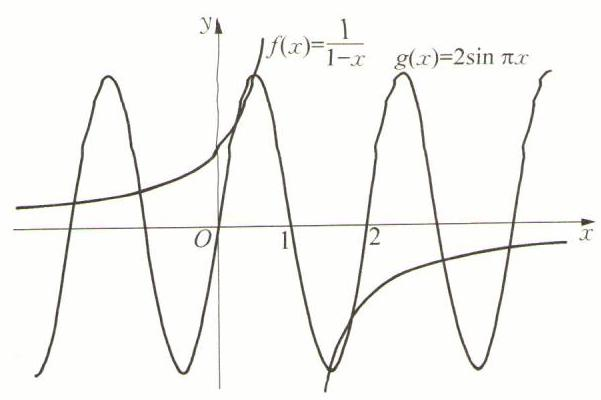
\includegraphics[max width=0.5\textwidth]{images/bo_d29ci7n7aajc738p8c80_28_900_139_601_400_0.jpg}
\end{center}
\hspace*{3em} 

第 1 题图

2.【答案】 $\left( {-\dfrac{2}{3},\dfrac{70}{27}}\right)$

【解析】设 $A\left( {m,n}\right)$ 为 $f\left( x\right)$ 图象的一个对称中心,则有等式 $f\left( x\right)  + f\left( {{2m} - x}\right)  = {2n}$ 恒成立,即 $\left( {{x}^{3} + 2{x}^{2} + {3x} + 4}\right)  + \left\lbrack  {{\left( 2m - x\right) }^{3} + 2{\left( 2m - x\right) }^{2} + 3\left( {{2m} - x}\right)  + 4}\right\rbrack   = {2n}$ 恒成立. 将该等式化简,欲使其恒成立,必须为 $0{x}^{3} + 0{x}^{2} + {0x} + {2n} = {2n}$ 的形式,故可解得 $m =  - \dfrac{2}{3}$ , $n = \dfrac{70}{27}.$

3.【答案】A

【解析】函数 $f\left( x\right)  = \dfrac{1}{x} + \dfrac{1}{x - 2} + \dfrac{1}{x - 4} + 3$ 定义域为 $\left( {-\infty ,0}\right)  \cup  \left( {0,2}\right)  \cup  \left( {2,4}\right)  \cup  (4$ , $+ \infty )$ ,其图象是由 4 条曲线组成,在区间 $\left( {-\infty ,0}\right) ,\left( {0,2}\right) ,\left( {2,4}\right) ,\left( {4, + \infty }\right)$ 上都单调递减.

由 $f\left( {4 - x}\right)  + f\left( x\right)  = \left( {-\dfrac{1}{x - 4} - \dfrac{1}{x - 2} - \dfrac{1}{x} + 3}\right)  + \left( {\dfrac{1}{x} + \dfrac{1}{x - 2} + \dfrac{1}{x - 4} + 3}\right)  = 6$ ,即 $f\left( x\right)$ 的图象关于点(2,3)对称.

根据 $f\left( x\right)$ 的单调性、对称性及极限值,可画出其函数的图象. 函数 $g\left( x\right)  = 4 - \dfrac{8}{{2}^{x} + 4}$ 定义域为 $\mathbf{R}$ ,在 $\mathbf{R}$ 上单调递增,值域为 $\left( {2,4}\right) ,g\left( {4 - x}\right)  + g\left( x\right)  = \left( {4 - \dfrac{8}{{2}^{4 - x} + 4}}\right)  + (4 -$  $\left. \dfrac{8}{{2}^{x} + 4}\right)  = 8 - \left( {\dfrac{2 \cdot  {2}^{x}}{{2}^{x} + 4} + \dfrac{8}{{2}^{x} + 4}}\right)  = 6,g\left( x\right)$ 的图象关于点 (2,3) 对称. 根据其单调性、对称性及极限值, 可作出其函数的图象.

根据图象,两图象一共有 4 个交点,它们关于点 (2,3) 对称,不妨令点 $\left( {{x}_{1},{y}_{1}}\right)$ 与 $\left( {{x}_{4},{y}_{4}}\right)$ 相互对称, $\left( {{x}_{2},{y}_{2}}\right)$ 与 $\left( {{x}_{3},{y}_{3}}\right)$ 相互对称,则 ${x}_{1} + {x}_{4} = {x}_{2} + {x}_{3} = 4,{y}_{1} + {y}_{4} = {y}_{2} + {y}_{3} =$ 6,所以 $\mathop{\sum }\limits_{{i = 1}}^{4}\left( {{x}_{i} + {y}_{i}}\right)  = {20}$ .

\begin{center}
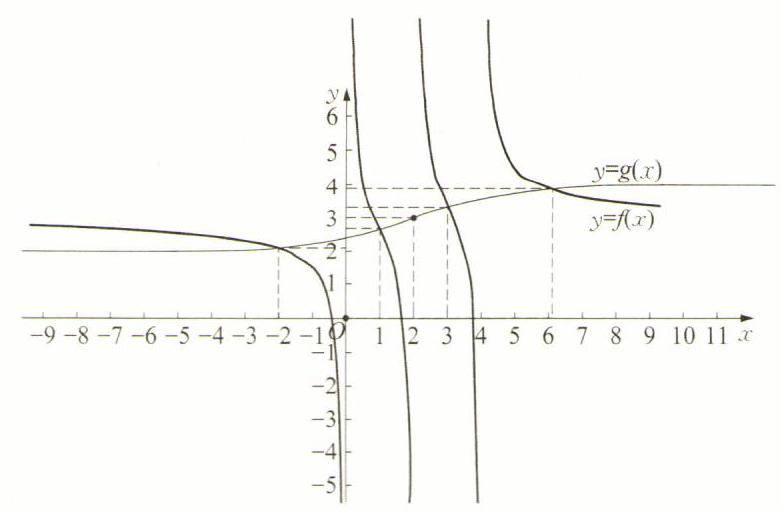
\includegraphics[max width=0.6\textwidth]{images/bo_d29ci7n7aajc738p8c80_29_428_154_781_511_0.jpg}
\end{center}
\hspace*{3em} 

第 3 题图

4.【答案】B

【解析】令 $x =  - 3$ ,有 $f\left( {-3 + 6}\right)  = f\left( {-3}\right)  + f\left( 3\right)$ ,又 $f\left( x\right)$ 是 $\mathbf{R}$ 上的偶函数,所以 $f\left( 3\right)  =$ 0,则有 $f\left( {x + 6}\right)  = f\left( x\right)$ ,所以 $f\left( x\right)$ 的周期为 6 .

对于 ①,函数为偶函数,则函数关于 $y$ 轴对称,又由函数的周期为 6,则直线 $x =  - 6$ 是函数 $f\left( x\right)$ 图象的一条对称轴,① 正确;

对于 ②,当 ${x}_{1},{x}_{2} \in  \left\lbrack  {0,3}\right\rbrack$ ,且 ${x}_{1} \neq  {x}_{2}$ 时,都有 $\dfrac{f\left( {x}_{1}\right)  - f\left( {x}_{2}\right) }{{x}_{1} - {x}_{2}} > 0$ ,则函数 $y = f\left( x\right)$ 在 [0,3]上为增函数,根据函数的对称性和周期性等性质,所以函数 $y = f\left( x\right)$ 在 $\left\lbrack  {-9, - 6}\right\rbrack$ 上为减函数, ② 错误;

对于 ③,在 $f\left( {x + 6}\right)  = f\left( x\right)  + f\left( 3\right)$ 式中,令 $x = 0$ ,又因为 $f\left( 3\right)  = 0$ ,函数 $y = f\left( x\right)$ 在 $\left\lbrack  {0,3}\right\rbrack$ 上为严格增函数,故 $f\left( 0\right)  \neq  0$ ,故函数 $y = f\left( x\right)$ 在 $\left\lbrack  {-9,9}\right\rbrack$ 上零点个数一定是偶数个, ③ 错误.

【补充说明】此题也可根据函数的周期性、图象的对称性等性质, 画出草图(如图)快速判断选项正误.

\begin{center}
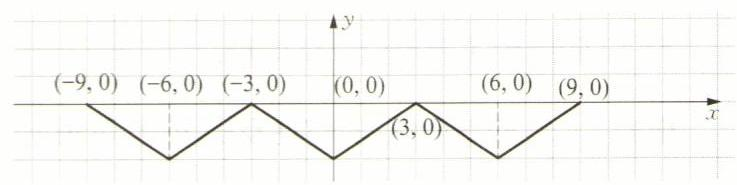
\includegraphics[max width=0.6\textwidth]{images/bo_d29ci7n7aajc738p8c80_29_760_1405_737_185_0.jpg}
\end{center}
\hspace*{3em} 

第 4 题图

5.【答案】B

【解析】因为 $f\left( {x + 6}\right)  + f\left( x\right)  = {2f}\left( 3\right)$ ,所以 $f\left( x\right)  + f\left( {x - 6}\right)  = {2f}\left( 3\right)$ ,故 $f\left( {x + 6}\right)  =$  $f\left( {x - 6}\right)$ ,所以函数的周期 $T = {12}$ . 2022 $= {12} \times  {168} + 6$ ,所以 $f\left( {2022}\right)  = f\left( 6\right)$ . 因为 $y =$  $f\left( {x - 1}\right)$ 的图象关于点 (1,0) 对称,所以 $y = f\left( x\right)$ 的图象关于点 (0,0) 对称,所以 $y =$  $f\left( x\right)$ 为奇函数,所以 $f\left( {-6}\right)  =  - f\left( 6\right)$ ,又因为 $y = f\left( x\right)$ 周期 $T = {12}$ ,所以 $f\left( {-6}\right)  = f\left( 6\right)$ , 所以 $f\left( 6\right)  = 0$ .

\section*{6.【答案】D}

【解析】因为 $f\left( {x + 1}\right)$ 是奇函数,所以 $f\left( {-x + 1}\right)  =  - f\left( {x + 1}\right) \cdots$ ①.

因为 $f\left( {x + 2}\right)$ 是偶函数,所以 $f\left( {x + 2}\right)  = f\left( {-x + 2}\right) \cdots$ ②.

令 $x = 1$ ,由 ① 得 $f\left( 0\right)  =  - f\left( 2\right)  =  - \left( {{4a} + b}\right)$ ,由 ② 得 $f\left( 3\right)  = f\left( 1\right)  = a + b$ ,因为 $f\left( 0\right)  +$  $f\left( 3\right)  = 6$ ,所以 $- \left( {{4a} + b}\right)  + a + b = 6 \Rightarrow  a =  - 2$ . 令 $x = 0$ ,由①得 $f\left( 1\right)  =  - f\left( 1\right)  \Rightarrow  f\left( 1\right)  =$  $0 \Rightarrow  b = 2$ ,所以 $f\left( x\right)  =  - 2{x}^{2} + 2$ . 于是 $f\left( \dfrac{9}{2}\right)  = f\left( {\dfrac{5}{2} + 2}\right)  = f\left( {-\dfrac{5}{2} + 2}\right)  = f\left( {-\dfrac{1}{2}}\right)  =$  $f\left( {-\dfrac{3}{2} + 1}\right)  =  - f\left( {\dfrac{3}{2} + 1}\right)  =  - f\left( \dfrac{5}{2}\right)  =  - f\left( {\dfrac{1}{2} + 2}\right)  =  - f\left( {-\dfrac{1}{2} + 2}\right)  =  - f\left( \dfrac{3}{2}\right)  = \dfrac{5}{2}.$

说明:从函数的周期性入手. 由两个函数图象的对称性可知,函数 $f\left( x\right)$ 的周期 $T = 4$ ,所以 $f\left( \dfrac{9}{2}\right)  = f\left( \dfrac{1}{2}\right)  =  - f\left( \dfrac{3}{2}\right)  = \dfrac{5}{2}.$

7.【答案】 ${C}$

【解析】由 $f\left( x\right)  + g\left( {2 - x}\right)  = 1$ 得 $f\left( {-x}\right)  + g\left( {2 + x}\right)  = 1$ ,又 $f\left( x\right)$ 为偶函数,所以 $g(2 -$  $x) = g\left( {2 + x}\right)$ ,即 $g\left( x\right)$ 的图象关于 $x = 2$ 对称; 又 $g\left( x\right)  - f\left( {x - 4}\right)  = 3$ 得 $g\left( {8 - x}\right)  -$  $f\left( {4 - x}\right)  = 3$ ,又 $f\left( x\right)$ 为偶函数,所以 $g\left( x\right)  = g\left( {8 - x}\right)$ ,即 $g\left( x\right)$ 的图象关于 $x = 4$ 对称; 因此 $g\left( x\right)  = g\left( {4 - x}\right)  = g\left( {4 + x}\right)$ ,所以 $g\left( x\right)$ 是以 4 为周期的周期函数,故 ${D}$ 错误.

因为 $f\left( x\right)  + g\left( {2 - x}\right)  = 1$ ,所以 $f\left( x\right)  = 1 - g\left( {2 - x}\right)  = 1 - \left\lbrack  {3 + f\left( {-2 - x}\right) }\right\rbrack   =  - f( - 2 -$  $x) - 2$ ,因此 $f\left( x\right)$ 的图象关于(-1, - 1)对称,故 ${B}$ 错误.

因为 $g\left( x\right)$ 是以 4 为周期的周期函数,所以 $f\left( x\right)  = 1 - g\left( {2 - x}\right)  = 1 - g\left( {6 - x}\right)  = 1 - \lbrack 3 +$  $f\left( {2 - x}\right) \rbrack  =  - f\left( {2 - x}\right)  - 2$ ,因此 $f\left( x\right)$ 的图象关于(1, - 1)对称,所以函数 $f\left( x\right)$ 是以 4 为周期的周期函数,故 ${C}$ 正确.

根据 $f\left( x\right)$ 是以 4 为周期的周期函数,由 $f\left( x\right)  + g\left( {2 - x}\right)  = 1,g\left( x\right)  - f\left( {x - 4}\right)  = 3$ ,得 $g\left( x\right)  + g\left( {2 - x}\right)  = 4$ ,所以函数 $g\left( x\right)$ 的图象关于 (1,2) 对称,故 ${A}$ 错误.

8.【答案】①②

【解析】对于①:因为函数 $f\left( x\right)$ 满足 $f\left( {x + 1}\right)  = f\left( {x - 1}\right)$ , 所以函数 $f\left( x\right)$ 为周期为 2 的函数,又因为函数为偶函数, 图象关于 $y$ 轴对称,所以 $f\left( x\right)$ 也关于直线 $x =  - 4$ 对称,故 ① 正确.

\begin{center}
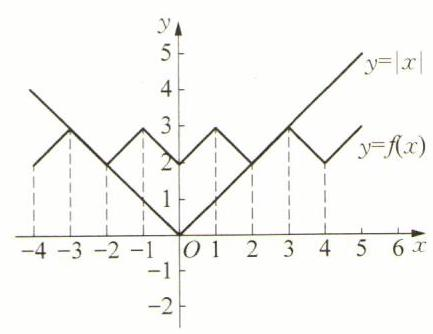
\includegraphics[max width=0.3\textwidth]{images/bo_d29ci7n7aajc738p8c80_30_1077_1575_433_334_0.jpg}
\end{center}
\hspace*{3em} 

第 8 题图

对于 ②: 方程 $f\left( x\right)  - \left| {x - a}\right|  = 0$ 一定有解,即函数 $f\left( x\right)$ 的图象与函数 $y = \left| {x - a}\right|$ 的图象一定有交点. 在同一个直角坐标系中作出两个函数 $y = \left| x\right|$ 与 $y = f\left( x\right)$ 的图象如图所示. 由图象可得,将 $y =  \mid  x \mid$ 左右平移后一定会与函数 $y = f\left( x\right)$ 相交,故 ② 正确.

对于 ③: 如图,若 $x = 2$ 为 $y = f\left( x\right)$ 与 $y = \left| {x - a}\right|$ 的一个交点,则当 $a = 0$ 时, $y = \left| x\right|$ 与 $y = f\left( x\right)$ 的图象都关于 $y$ 轴对称,所有交点的横坐标之和为 0,故 ③ 错误.

对于 ④:若关于 $x$ 的不等式 $f\left( x\right)  - \left| {x - a}\right|  < 0$ 在区间 $\lbrack 0, + \infty )$ 上恒成立,即 $\left| {x - a}\right|  >$  $f\left( x\right)$ 恒成立,通过图象的平移可知, $a <  - 2$ ,即实数 $a$ 没有最大值,故 ④ 错误.

9.【答案】 ${C}$

【解析】函数 $f\left( x\right)$ 关于点 $M\left( {0,1}\right)$ 对称,这显然也是正方形的对称中心,由正方形性质可得, ${AC} \bot  {BD}$ 于 $M$ ,且 $\left| {AM}\right|  = \left| {BM}\right|  = \left| {CM}\right|  = \left| {DM}\right|$ ,不妨设直线 ${AC}$ 的方程为 $y = {kx}$ 十 $1\left( {k > 0}\right)$ ,则直线 ${BD}$ 方程为 $y =  - \dfrac{1}{k}x + 1$ ,设 $A\left( {{x}_{1},{y}_{1}}\right) ,B\left( {{x}_{2},{y}_{2}}\right)$ ,则 $C\left( {-{x}_{1},2 - }\right.$  $\left. {y}_{1}\right) ,D\left( {-{x}_{2},2 - {y}_{2}}\right)$ ,联立直线 ${AC}$ 与函数 $y = f\left( x\right)$ 得 $\left\{  \begin{array}{l} y = {kx} + 1, \\  y = {x}^{3} - \dfrac{9}{2}x + 1, \end{array}\right.$ 可得 ${x}^{3} -$  $\left( {k + \dfrac{9}{2}}\right) x = 0$ ,所以 ${x}_{1}^{2} = k + \dfrac{9}{2}$ ,同理 ${x}_{2}^{2} = \dfrac{9}{2} - \dfrac{1}{k}$ ,又 $\left| {AM}\right|  = \sqrt{1 + {k}^{2}}\left| {{x}_{1} - 0}\right| ,\left| {BM}\right|  =$  $\sqrt{1 + \dfrac{1}{{k}^{2}}}\left| {{x}_{2} - 0}\right|$ ,所以 $\left( {1 + {k}^{2}}\right) \left( {k + \dfrac{9}{2}}\right)  = \left( {1 + \dfrac{1}{{k}^{2}}}\right) \left( {\dfrac{9}{2} - \dfrac{1}{k}}\right)$ ,即 ${k}^{2} + \dfrac{1}{{k}^{2}} + \dfrac{9}{2}\left( {k - \dfrac{1}{k}}\right)  = 0$ , 整理得 $2{\left( k - \dfrac{1}{k}\right) }^{2} + 9\left( {k - \dfrac{1}{k}}\right)  + 4 = 0$ ,解得 $k - \dfrac{1}{k} =  - 4$ 或 $k - \dfrac{1}{k} =  - \dfrac{1}{2}$ ,所以 $k + \dfrac{1}{k} =$  $\sqrt{{\left( k - \dfrac{1}{k}\right) }^{2} + 4} = 2\sqrt{5}$ 或 $\dfrac{\sqrt{17}}{2}$ ,所以 ${S}_{ABCD} = 2\left| {AM}\right| \left| {BM}\right|  = 2\sqrt{1 + {k}^{2}} \cdot  \sqrt{1 + \dfrac{1}{{k}^{2}}} \cdot  \left| {{x}_{1}{x}_{2}}\right|  =$  $2\left( {k + \dfrac{1}{k}}\right)  \cdot  \sqrt{\left( {k + \dfrac{9}{2}}\right) \left( {\dfrac{9}{2} - \dfrac{1}{k}}\right) } = 2\left( {k + \dfrac{1}{k}}\right) \sqrt{\dfrac{9}{2}\left( {k - \dfrac{1}{k}}\right)  + \dfrac{77}{4}} = {10}$ 或 17.

10.【答案】D

【解析】由题意可知,函数 $f\left( x\right)  = \dfrac{x}{x + 1} + \dfrac{x + 1}{x + 2} + \dfrac{x + 2}{x + 3} = \left( {1 - \dfrac{1}{x + 1}}\right)  + \left( {1 - \dfrac{1}{x + 2}}\right)  +$  $\left( {1 - \dfrac{1}{x + 3}}\right)  = 3 - \left( {\dfrac{1}{x + 1} + \dfrac{1}{x + 2} + \dfrac{1}{x + 3}}\right)$ ,其定义域为 $\{ x \mid  x \neq   - 1,x \neq   - 2,x \neq   - 3\}$ .

对于 ①:显然函数在 $x \in  \left( {-2, - 1}\right)$ 内连续且严格单调递增,当 $x \rightarrow   - {2}^{ + }$ 时, $f\left( x\right)  \rightarrow$  $- \infty$ ,当 $x \rightarrow   - {1}^{ - }$ 时, $f\left( x\right)  \rightarrow   + \infty$ ,可知函数的值域是 $\mathbf{R}$ ,所以 ① 正确.

对于 ②: 因为 $f\left( x\right)  = \dfrac{x}{x + 1} + \dfrac{x + 1}{x + 2} + \dfrac{x + 2}{x + 3} = 3 - \left( {\dfrac{1}{x + 1} + \dfrac{1}{x + 2} + \dfrac{1}{x + 3}}\right)$ ,显然函数在 $\left( {-\infty , - 3}\right) ,\left( {-3, - 2}\right) ,\left( {-2, - 1}\right) ,\left( {-1, + \infty }\right)$ 四个区间内连续且严格单调递增,如 ① 分析各区间端点的极限值,根据零点存在性定理,可知 $f\left( x\right)$ 在定义域内有三个零点,所以 ② 正确.

对于 ③: 因为 $f\left( x\right)  = 3 - \left( {\dfrac{1}{x + 1} + \dfrac{1}{x + 2} + \dfrac{1}{x + 3}}\right)$ ,所以 $f\left( {-4 - x}\right)  = 3 + \left( {\dfrac{1}{x + 1} + \dfrac{1}{x + 2} + }\right.$

$\left. \dfrac{1}{x + 3}\right)  = 6 - \left\lbrack  {3 - \left( {\dfrac{1}{x + 1} + \dfrac{1}{x + 2} + \dfrac{1}{x + 3}}\right) }\right\rbrack   = 6 - f\left( x\right)$ ,得 $f\left( x\right)  + f\left( {-4 - x}\right)  = 6$ ,即函数的图象关于点(-2,3)中心对称,所以 ③ 正确.

11.【答案】 $\dfrac{1}{2} \leq  t \leq  \dfrac{7}{2}$

【解析】定义在 $\mathbf{R}$ 上的奇函数 $f\left( x\right)$ 满足 $f\left( 0\right)  = 0$ ,则 ${\log }_{2}a = 0$ ,则 $a = 1$ ,又由 $f\left( {x + 2}\right)  =$  $- f\left( x\right)$ ,可得 $f\left( x\right)  =  - f\left( {x + 2}\right)  = f\left( {x + 4}\right)$ ,则 4 为函数 $f\left( x\right)$ 的一个周期,由 $f\left( {x + 2}\right)  =$  $- f\left( x\right)  = f\left( {-x}\right)$ ,可得 $f\left( x\right)$ 的图象有对称轴 $x = 1$ ,当 $0 \leq  x \leq  1$ 时, $f\left( x\right)  = {\log }_{2}\left( {x + 1}\right)$ . 根据 $f\left( x\right)$ 在 $0 \leq  x \leq  1$ 时的解析式及相关对称性、周期性,易作出 $f\left( x\right)$ 在 $\mathbf{R}$ 上的图象,如图所示.

\begin{center}
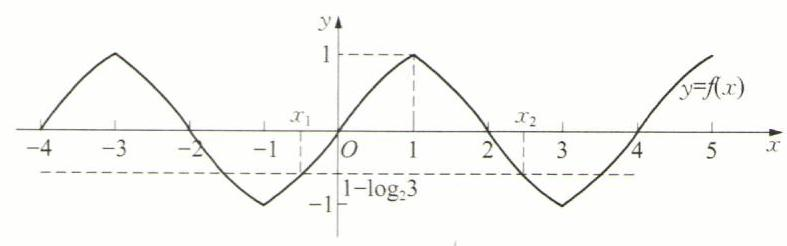
\includegraphics[max width=0.6\textwidth]{images/bo_d29ci7n7aajc738p8c80_32_435_769_787_246_0.jpg}
\end{center}
\hspace*{3em} 

第 11 题图

设 $- 1 < {x}_{1} < 0 < 2 < {x}_{2} < 3$ 且 $f\left( {x}_{1}\right)  = f\left( {x}_{2}\right)  = 1 - {\log }_{2}3$ . 由奇函数 $f\left( x\right)$ 的图象关于原点对称,可得 $f\left( {x}_{1}\right)  =  - f\left( {-{x}_{1}}\right)  =  - {\log }_{2}\left( {-{x}_{1} + 1}\right)  = 1 - {\log }_{2}3$ ,解得 ${x}_{1} =  - \dfrac{1}{2}$ . 根据 $f\left( x\right)$ 的图象关于 $x = 1$ 对称,可得 ${x}_{2} = \dfrac{5}{2}$ . 因为对于任意 $x \in  \left\lbrack  {0,1}\right\rbrack$ ,都有 $f\left( {-{x}^{2} + {tx}}\right)  \geq  1 - {\log }_{2}3$ ,所以对于任意 $x \in  \left\lbrack  {0,1}\right\rbrack$ ,都有 $- {x}^{2} + {tx} \in$  $\left\lbrack  {-\dfrac{1}{2} + {4k},\dfrac{5}{2} + {4k}}\right\rbrack$ ,其中 $k \in  \mathbf{Z}$ . 因为 $x = 0$ 时, $- {x}^{2} + {tx} = 0$ ,故 $k = 0$ ,即对于任意 $x$

$\in  \left\lbrack  {0,1}\right\rbrack$ ,都有 $- {x}^{2} + {tx} \in  \left\lbrack  {-\dfrac{1}{2},\dfrac{5}{2}}\right\rbrack$ . 显然当 $x = 0$ 时, $- {x}^{2} + {tx} \in  \left\lbrack  {-\dfrac{1}{2},\dfrac{5}{2}}\right\rbrack$ ; 当 $x$  $\in  (0,1\rbrack$ 时, $- {x}^{2} + {tx} \in  \left\lbrack  {-\dfrac{1}{2},\dfrac{5}{2}}\right\rbrack   \Leftrightarrow   - \dfrac{1}{2} \leq   - {x}^{2} + {tx} \leq  \dfrac{5}{2} \Leftrightarrow  {x}^{2} - \dfrac{1}{2} \leq  {tx} \leq  {x}^{2} +$  $\dfrac{5}{2} \Leftrightarrow  x - \dfrac{1}{2x} \leq  t \leq  x + \dfrac{5}{2x}$ 恒成立,解之得 $\dfrac{1}{2} \leq  t \leq  \dfrac{7}{2}$ . 综上,实数 $t$ 的取值范围为 $\dfrac{1}{2} \leq  t \leq$  $\dfrac{7}{2}$ .

\section*{11 函数的图象}

1.【答案】B

【解析】画出函数 $y = \dfrac{x}{x - 1}$ 的图象(如图 1); 保留函数 $y = \dfrac{x}{x - 1}$ 在 $\lbrack 0, + \infty )$ 上的图象,并把它关于 $y$ 轴对称到 $y$ 轴左侧得到函数 $y = \dfrac{\left| x\right| }{\left| x\right|  - 1}$ 的图象 (如图 2); 再把函数 $y = \dfrac{\left| x\right| }{\left| x\right|  - 1}$ 在 $x$ 轴下方区域的图象关于 $x$ 轴对称到 $x$ 轴上方得到函数 $f\left( x\right)  = \dfrac{\left| x\right| }{\left| \right| x\left| {-1}\right| }$ 的图象 (如图 3). 根据图象,易知①③ 错,④正确. 因为 $y = {kx} + b\left( {k \neq  0}\right)$ 的图象是一条既不是水平横着也不是竖着的直线,故方程 $f\left( x\right)  = {kx} + b\left( {k \neq  0}\right)$ 一定有解,② 正确.

\begin{center}
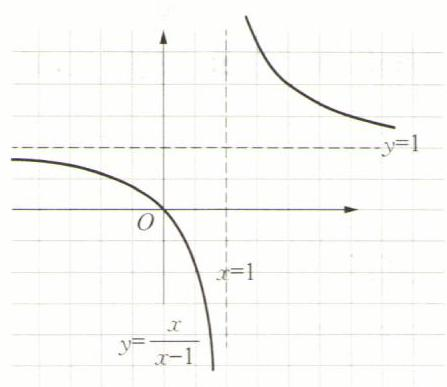
\includegraphics[max width=0.3\textwidth]{images/bo_d29ci7n7aajc738p8c80_33_133_572_447_387_0.jpg}
\end{center}
\hspace*{3em} 

第 1 题图 1

\begin{center}
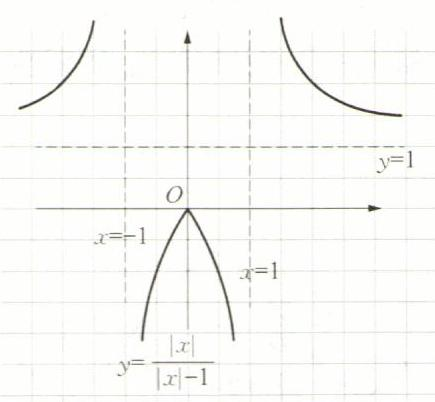
\includegraphics[max width=0.3\textwidth]{images/bo_d29ci7n7aajc738p8c80_33_594_573_435_402_0.jpg}
\end{center}
\hspace*{3em} 

第 1 题图 2

\begin{center}
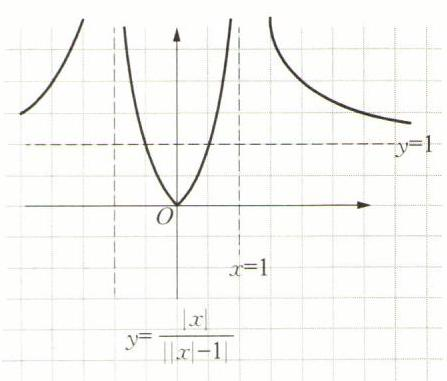
\includegraphics[max width=0.3\textwidth]{images/bo_d29ci7n7aajc738p8c80_33_1046_575_447_381_0.jpg}
\end{center}
\hspace*{3em} 

第 1 题图 3

2.【答案】7

【解析】函数 $y = {f}_{2}\left( x\right)$ 的图象如图的实线部分所示,所求的封闭部分的面积为 ${S}_{\text{ 梯形 ABCD }} - {S}_{\bigtriangleup {CDE}} = \dfrac{1}{2}\left( {2 + 6}\right)  \times  2 -$  $\dfrac{1}{2} \times  2 \times  1 = 7.$

\begin{center}
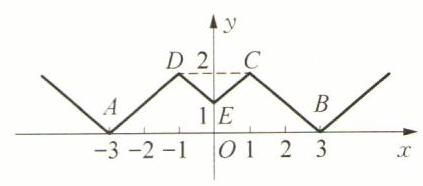
\includegraphics[max width=0.3\textwidth]{images/bo_d29ci7n7aajc738p8c80_33_1069_1143_423_186_0.jpg}
\end{center}
\hspace*{3em} 

第 2 题图

3.【答案】 -1 或 2

【解析】先作出函数 $f\left( x\right)  = \dfrac{x - 2}{x + 2}$ 的图象,如图 1 ; 再把 $f\left( x\right)  = \dfrac{x - 2}{x + 2}$ 在 $y$ 轴右半部分的图象沿着 $y$ 轴翻折,得到 $y = f\left( \left| x\right| \right)$ 的图象,如图 2 ; 然后把 $y =$  $f\left( \left| x\right| \right)$ 的在 $x$ 轴下面的图象沿着 $x$ 轴翻折,得到 $y = \left| {f\left( \left| x\right| \right) }\right|$ 的图象,如图 3 ; 截取函数 $y =$  $\left| {f\left( \left| x\right| \right) }\right|$ 在区间 $\left\lbrack  {-1,2}\right\rbrack$ 的图象,可知把此函数向上平移 1 个单位或向下平移 2 个单位时,函数 $y =$  $\left| \right| f\left( \left| x\right| \right) \left| {-t}\right|$ 在 $\left\lbrack  {-1,2}\right\rbrack$ 的最大值为 2,即 $t =  - 1$ 或 2.

\begin{center}
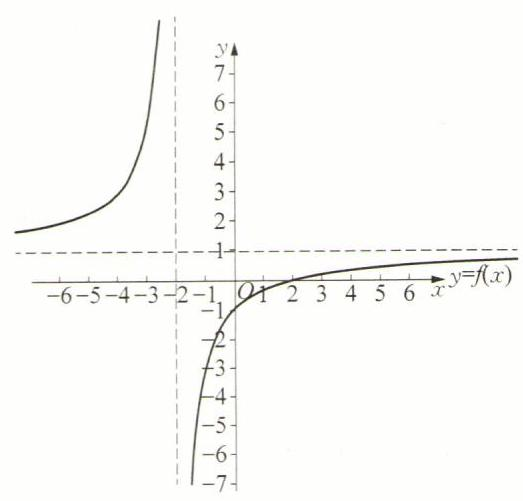
\includegraphics[max width=0.4\textwidth]{images/bo_d29ci7n7aajc738p8c80_33_970_1525_523_501_0.jpg}
\end{center}
\hspace*{3em} 

第 3 题图 1

\begin{center}
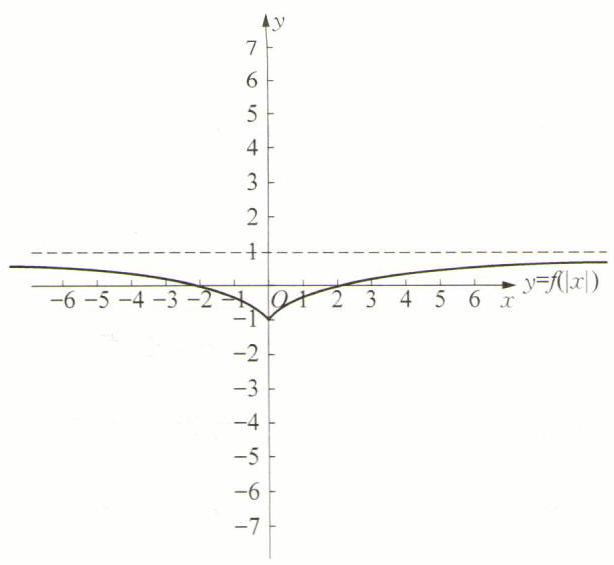
\includegraphics[max width=0.5\textwidth]{images/bo_d29ci7n7aajc738p8c80_34_167_152_614_565_0.jpg}
\end{center}
\hspace*{3em} 

第 3 题图 2

\begin{center}
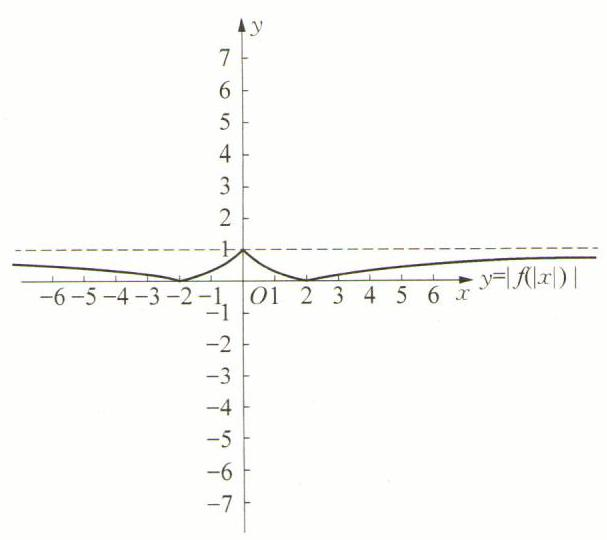
\includegraphics[max width=0.5\textwidth]{images/bo_d29ci7n7aajc738p8c80_34_876_174_607_540_0.jpg}
\end{center}
\hspace*{3em} 

第 3 题图 3

4.【答案】 $\left( {-\dfrac{1}{2},0}\right)  \cup  \left( {0,\dfrac{1}{2}}\right)$

【解析】不妨令 $y = {\left( \dfrac{1}{2}\right) }^{{2x} - 1} - {x}^{\alpha }$ ,由 $\alpha  > 0$ ,易知 $y = {\left( \dfrac{1}{2}\right) }^{{2x} - 1} - {x}^{\alpha }$ 在 $(0,1\rbrack$ 上单调递减. 当 $x \rightarrow  0$ 时, $y \rightarrow  2$ ; 当 $x = 1$ 时, $y =  - \dfrac{1}{2}$ . 故 $y = {\left( \dfrac{1}{2}\right) }^{{2x} - 1} - {x}^{\alpha }$ 在 $(0,1\rbrack$ 上的大致图象如图 1 所示.

\begin{center}
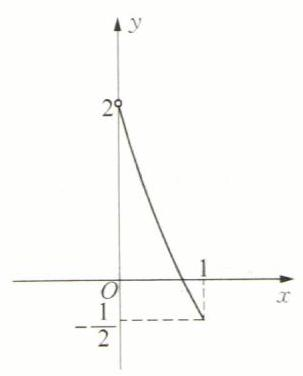
\includegraphics[max width=0.2\textwidth]{images/bo_d29ci7n7aajc738p8c80_34_278_1239_303_376_0.jpg}
\end{center}
\hspace*{3em} 

第 4 题图 1

\begin{center}
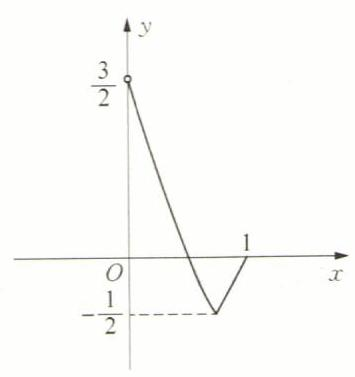
\includegraphics[max width=0.3\textwidth]{images/bo_d29ci7n7aajc738p8c80_34_658_1235_355_377_0.jpg}
\end{center}
\hspace*{3em} 

第 4 题图 2

\begin{center}
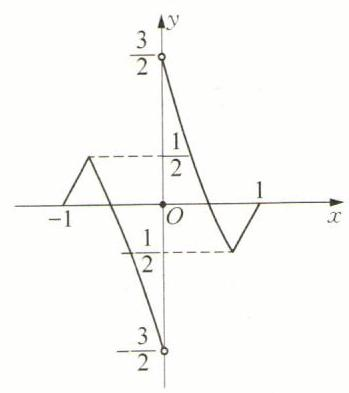
\includegraphics[max width=0.2\textwidth]{images/bo_d29ci7n7aajc738p8c80_34_1091_1211_349_393_0.jpg}
\end{center}
\hspace*{3em} 

第 4 题图 3

由函数图象平移变换和对称变换,得 $f\left( x\right)  = \left| {{\left( \dfrac{1}{2}\right) }^{{2x} - 1} - {x}^{a}}\right|  - \dfrac{1}{2}$ 在 $(0,1\rbrack$ 上的大致图象如图 2 所示.

又因为 $f\left( x\right)$ 为奇函数,所以 $f\left( x\right)$ 在 $\left\lbrack  {-1,1}\right\rbrack$ 上的图象如图 3 所示.

因为 $g\left( x\right)  = f\left( x\right)  - t$ 有 3 个零点等价于 $f\left( x\right)$ 的图象与 $y = t$ 有三个不同的交点,所以 $- \dfrac{1}{2} < t < 0$ 或 $0 < t < \dfrac{1}{2}$ ,即实数 $t$ 的取值范围为 $\left( {-\dfrac{1}{2},0}\right)  \cup  \left( {0,\dfrac{1}{2}}\right)$ .

5.【答案】 $\left\lbrack  {\dfrac{1}{{e}}, + \infty }\right)$

【解析】 $f\left( x\right)  = \dfrac{{{e}}^{-\left| {2 - x}\right| }}{x - 2\sqrt{x - 1}} - a$ 的定义域为 $\lbrack 1,2) \cup  \left( {2, + \infty }\right)$ ,则其函数 $f\left( x\right)$ 在 $\lbrack 1,2) \cup$ (2,5)内有两个零点,等价于方程 $\dfrac{{{e}}^{-\left| {2 - x}\right| }}{x - 2\sqrt{x - 1}} - a = 0$ 在 $\lbrack 1,2) \cup  \left( {2,5}\right)$ 上有两个根,等价于 $y = {{e}}^{\left| 2 - x\right| }$ ( $x - 2\sqrt{x - 1}$ ) 和 $y = \dfrac{1}{a}$ 在 $\lbrack 1,2) \cup  \left( {2,5}\right)$ 上的图象有两个交点. 令 $t =$  $\sqrt{x - 1} \in  \lbrack 0,1) \cup  \left( {1,2}\right)$ ,则 $x = {t}^{2} + 1$ ,故 $y = {{e}}^{\left| 1 - {t}^{2}\right| }{\left( t - 1\right) }^{2}$ ,原题等价于 $y =$  ${{e}}^{\left| 1 - {t}^{2}\right| }{\left( t - 1\right) }^{2}$ 和 $y = \dfrac{1}{a}$ 在 $\lbrack 0,1) \cup  \left( {1,2}\right)$ 上的图象有两个交点. 设 $g\left( t\right)  = {{e}}^{\left| 1 - {t}^{2}\right| }{\left( t - 1\right) }^{2} =$  $\left\{  \begin{array}{ll} {{e}}^{1 - {t}^{2}}{\left( t - 1\right) }^{2}, & 0 \leq  t < 1, \\  {{e}}^{{t}^{2} - 1}{\left( t - 1\right) }^{2}, & 1 < t < 2, \end{array}\right.$ 易得 $y = {{e}}^{1 - {t}^{2}}$ 和 $y = {\left( t - 1\right) }^{2}$ 在 $0 \leq$

\begin{center}
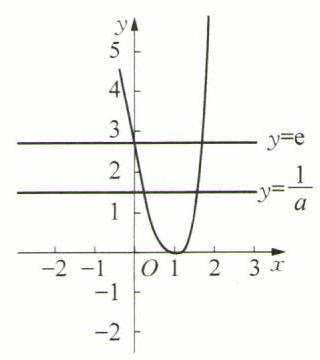
\includegraphics[max width=0.2\textwidth]{images/bo_d29ci7n7aajc738p8c80_35_1177_704_320_360_0.jpg}
\end{center}
\hspace*{3em} 

第 5 题图

$t < 1$ 时单调递减且均大于 0,故 $g\left( t\right)  = {{e}}^{1 - {t}^{2}}{\left( t - 1\right) }^{2}$ 在 $0 \leq  t < 1$ 时单调递减,同理可得 $g\left( t\right)  = {{e}}^{{t}^{2} - 1}{\left( t - 1\right) }^{2}$ 在 $1 < t < 2$ 时单调递增. 函数 $g\left( t\right)  = {{e}}^{\left| 1 - {t}^{2}\right| }{\left( t - 1\right) }^{2}$ 的图象如图所示,由 $g\left( 2\right)  = {{e}}^{3} > g\left( 0\right)  =$  ${e}$ ,结合图象可得 $0 < \dfrac{1}{a} \leq  {e}$ ,即 $a \geq  \dfrac{1}{{e}}$ .

6.【答案】 $a \leq   - \dfrac{1}{2}$ 或 $a \geq  1$

【解析】设 $g\left( x\right)  = \dfrac{{x}^{2} + {ax} + a}{x} = x + \dfrac{a}{x} + a$ .

① 若 $a \leq  0$ ,此时 $g\left( x\right)  = x + \dfrac{a}{x} + a$ 在 $(0,1\rbrack$ 上严格单调递增,欲使 $f\left( x\right)  =$  $\left| \dfrac{{x}^{2} + {ax} + a}{x}\right|$ 在 $(0,1\rbrack$ 上单调递减,只需 $g\left( x\right)  \leq  0$ 在 $(0,1\rbrack$ 内恒成立即可,即 $g\left( 1\right)  \leq  0$ , 解得 $a \leq   - \dfrac{1}{2}$ .

② 若 $a > 0$ ,此时 $g\left( x\right)  = x + \dfrac{a}{x} + a$ 在 $\left( {0,\sqrt{a}}\right\rbrack$ 上严格单调递减,在 $\left\lbrack  {\sqrt{a}, + \infty }\right)$ 上严格单调递增,欲使 $f\left( x\right)  = \left| \dfrac{{x}^{2} + {ax} + a}{x}\right|$ 在 $(0,1\rbrack$ 上单调递减,只需 $\left\{  \begin{array}{l} \sqrt{a} \geq  1, \\  g\left( x\right)  \geq  0 \end{array}\right.$ 在 $(0,1\rbrack$ 内恒成立即可,即 $\left\{  \begin{array}{l} \sqrt{a} \geq  1, \\  g\left( 1\right)  \geq  0, \end{array}\right.$ 解得 $a \geq  1$ . 综上,实数 $a$ 的取值范围为 $a \leq   - \dfrac{1}{2}$ 或 $a \geq  1$ .

\section*{12 数形结合}

1.【答案】 ${C}$

【解析】若 $x \in  \left( {0,1}\right)$ ,则 $x - 1 \in  \left( {-1,0}\right) ,f\left( {x - 1}\right)  = \dfrac{1}{x} - 1$ , $f\left( x\right)  = \dfrac{1}{\dfrac{1}{x} - 1 + 1} = x$ ,根据函数的平移变换与翻折变换,画出 $\left| {f\left( x\right)  - \dfrac{1}{2}}\right|$ 在(-1,1)上的图象,则 $y = m\left( {x + 1}\right)$ 与 $y =$  $\left| {f\left( x\right)  - \dfrac{1}{2}}\right|$ 的图象有三个交点时,函数 $\left| {f\left( x\right)  - \dfrac{1}{2}}\right|  - {mx} -$  $m = 0$ 有三个零点,可得 ${k}_{AC} = \dfrac{\dfrac{1}{2}}{1 - \left( {-1}\right) } = \dfrac{1}{4},{k}_{AB} = \dfrac{\dfrac{1}{2}}{0 - \left( {-1}\right) } = \dfrac{1}{2},y = m\left( {x + 1}\right)$ 是斜率为 $m$ ,且过定点 $A\left( {-1,0}\right)$ 的直线,绕 $A\left( {-1,0}\right)$ 旋转直线,由图知,当 $\dfrac{1}{4} \leq  m < \dfrac{1}{2}$ 时,直线与曲线有三个交点,函数 $g\left( x\right)  = \left| {f\left( x\right)  - \dfrac{1}{2}}\right|  - {mx} - m$ 在(-1,1)内恰有 3 个零点,所以 $m$ 的取值范围是 $\left\lbrack  {\dfrac{1}{4},\dfrac{1}{2}}\right)$ .

\begin{center}
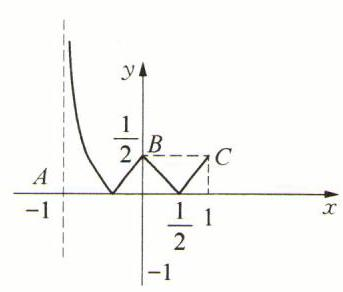
\includegraphics[max width=0.2\textwidth]{images/bo_d29ci7n7aajc738p8c80_36_1163_392_343_292_0.jpg}
\end{center}
\hspace*{3em} 

第 1 题图

2.【答案】 $\left( {-\dfrac{3}{5},\dfrac{1}{2}}\right)$

\begin{center}
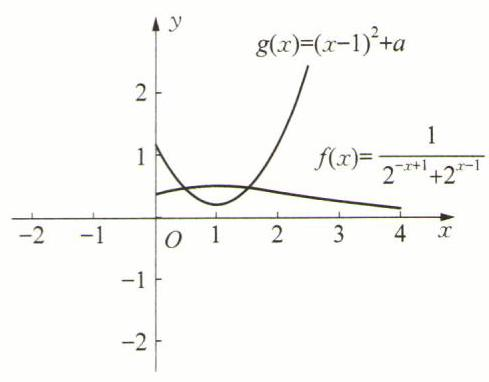
\includegraphics[max width=0.4\textwidth]{images/bo_d29ci7n7aajc738p8c80_36_1015_1292_489_382_0.jpg}
\end{center}
\hspace*{3em} 

第 2 题图

【解析】令 ${f}_{1}\left( x\right)  = {2}^{x - 1} + {2}^{-x + 1}$ ,则 ${f}_{1}\left( x\right)  = {2}^{x - 1} + {2}^{-x + 1}$ 是由 $t\left( x\right)  = {2}^{x} + {2}^{-x}$ 向右平移 1 个单位得到的,易得 ${f}_{1}\left( x\right)  = {2}^{x - 1} + {2}^{-x + 1}$ 关于 $x = 1$ 对称,且在 $\left( {-\infty ,1}\right)$ 上单调递减,在 $\left( {1, + \infty }\right)$ 上单调递增,所以当 $x > 0$ 时, 可作出 $f\left( x\right)  = \dfrac{1}{{2}^{x - 1} + {2}^{-x + 1}}\left( {x > 0}\right)$ 的大致图象如图所示.

若 $f\left( x\right)$ 图象仅有两对点关于 $y$ 轴对称,即 $f\left( x\right) \left( {x < 0}\right)$ 的图象关于 $y$ 轴对称的函数图象与 $f\left( x\right) \left( {x > 0}\right)$ 仅有两个交点,而当 $x < 0$ 时, $f\left( x\right)  = {\left( x + 1\right) }^{2} + a$ . 易得其关于 $y$ 轴对称的函数为 $g\left( x\right)  = {\left( -x + 1\right) }^{2} + a = {\left( x - 1\right) }^{2} + a\left( {x > 0}\right)$ ,大致图象如图所示,当 $g\left( x\right)$ 与 $f\left( x\right)$ 仅有两个交点时, $a + 1 > \dfrac{2}{5}$ 且 $a < \dfrac{1}{2}$ ,得 $- \dfrac{3}{5} < a < \dfrac{1}{2}$ .

综上, $a$ 的取值范围是 $\left( {-\dfrac{3}{5},\dfrac{1}{2}}\right)$ .

3.【答案】(4, $+ \infty$ )

【解析】由 $y = {3}^{\left| {\log }_{3}\left( x + 1\right) \right| }$ ,得 $y = \left\{  \begin{array}{ll} \dfrac{1}{x + 1}, &  - 1 < x < 0, \\  x + 1, & x \geq  0. \end{array}\right.$

\begin{center}
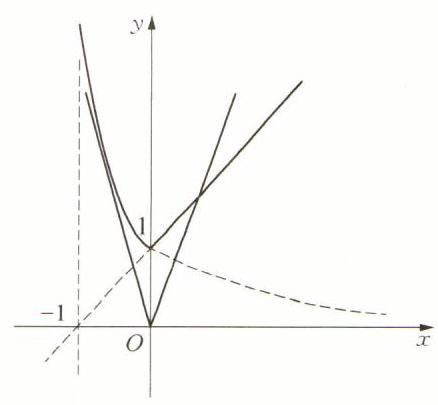
\includegraphics[max width=0.3\textwidth]{images/bo_d29ci7n7aajc738p8c80_37_1054_252_438_405_0.jpg}
\end{center}
\hspace*{3em} 

第 5 题图

作出两函数的图象如图所示.

当 $x \geq  0$ 时, $k > 1$ ,在 $\lbrack 0, + \infty )$ 上有且仅有一个交点,则当 $x < 0$ 时,两函数图象还得有且只有两个交点,即 $y =$  $- {kx}$ 与 $y = \dfrac{1}{x + 1}$ 在 $x < 0$ 时有两个交点. 先考虑临界状态,即 $y =  - {kx}$ 与 $y = \dfrac{1}{x + 1}$ 在 $x < 0$ 的某处相切时,令 $- {kx} = \dfrac{1}{x + 1}\left( {x < 0}\right)$ ,即 $k{x}^{2} + {kx} + 1 = 0$ ,使 $\Delta  = {k}^{2} - {4k} = 0$ ,解得 $k = 4$ 或 0 (舍去),于是当 $k > 4$ 时两函数总共有 3 个公共点.

4.【答案】D

【解析】 $y = a\left| x\right|$ 的图象为过原点的折线,关于 $y$ 轴对称,分三种情况讨论:① 当 $a > 0$ 时, $y = a\left| x\right|$ 的图象过第一、二象限,直线 $y = x + a$ 斜率为 1,当 $a > 0$ 时,直线 $y = x + a$ 过第一、二、三象限,若使其图象恰有两个公共点,如图 1,必有 $a > 1$ ；② 当 $a < 0$ 时, $y = a\left| x\right|$ 过第三、四象限; 而 $y = x + a$ 过第一、三、四象限,若使它们的图象恰有两个公共点,如图 2,必有 $a <  - 1$ . ③ 当 $a = 0$ 时,显然两函数只有一个公共点,不合题意.

\begin{center}
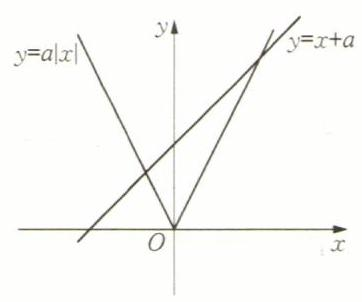
\includegraphics[max width=0.3\textwidth]{images/bo_d29ci7n7aajc738p8c80_37_379_1341_362_302_0.jpg}
\end{center}
\hspace*{3em} 

第 4 题图 1

\begin{center}
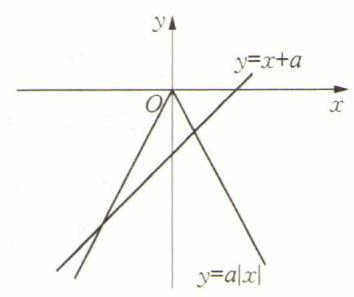
\includegraphics[max width=0.3\textwidth]{images/bo_d29ci7n7aajc738p8c80_37_897_1346_354_297_0.jpg}
\end{center}
\hspace*{3em} 

第 4 题图 2

5.【答案】A

【解析】显然 0 不是函数 $f\left( x\right)$ 的零点. $f\left( x\right)  = \left| {{x}^{2} - 4}\right|  + {x}^{2} + {kx} = 0 \Rightarrow  k = \dfrac{\left| {{x}^{2} - 4}\right|  + {x}^{2}}{-x}$ ,

即 $k = \left\{  \begin{array}{ll}  - \dfrac{4}{x}, & x \in  \left( {0,2}\right) , \\  \dfrac{4 - 2{x}^{2}}{x}, & x \in  \lbrack 2,4), \end{array}\right.$ 令 $g\left( x\right)  = \left\{  \begin{array}{ll}  - \dfrac{4}{x}, & x \in  \left( {0,2}\right) , \\  \dfrac{4 - 2{x}^{2}}{x}, & x \in  \lbrack 2,4). \end{array}\right.$ 函数 $f\left( x\right)$ 在区间

(0,4)上有两个不同的零点,转化为函数 $g\left( x\right)$ 的图象与直线 $y = k$ 在区间(0,4)上有两个交点,作出函数 $g\left( x\right)$ 的草图,如图所示. 由图可知, $k$ 的取值范围是 $- 7 < k <  - 2$ .

\begin{center}
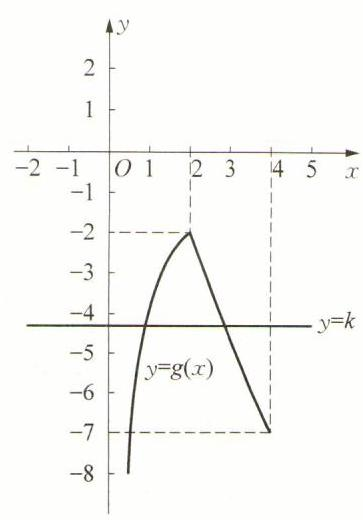
\includegraphics[max width=0.3\textwidth]{images/bo_d29ci7n7aajc738p8c80_38_1143_133_363_520_0.jpg}
\end{center}
\hspace*{3em} 

第 5 题图

6.【答案】D

【解析】函数 $g\left( x\right)  = f\left( x\right)  - \left| {k{x}^{2} - {2x}}\right| \left( {k \in  \mathbf{R}}\right)$ 恰有 4 个零点,即函数 $f\left( x\right)$ 与 $h\left( x\right)  = \left| {k{x}^{2} - {2x}}\right|$ 的图象有 4 个交点,易知(0,0)必为一个交点. 当 $x > 0$ 时,由 ${x}^{3} =$  $\left| {k{x}^{2} - {2x}}\right|$ 可得 ${x}^{2} = \left| {{kx} - 2}\right|$ ；当 $x < 0$ 时,由 $- x =$  $\left| {k{x}^{2} - {2x}}\right|$ 可得 $1 = \left| {{kx} - 2}\right|$ ,令 $\varphi \left( x\right)  = \left\{  \begin{array}{ll} {x}^{2}, & x > 0, \\  1, & x < 0, \end{array}\right.$  $\mu \left( x\right)  = \left| {{kx} - 2}\right|$ ,即函数 $\varphi \left( x\right)$ 与 $\mu \left( x\right)$ 的图象有 3 个交点. 若 $k < 0$ ,如图 1 所示,函数 $\varphi \left( x\right)$ 与 $\mu \left( x\right)$ 的图象有 3 个交点 (注意: $\mu \left( x\right)  = \left| {{kx} - 2}\right|$ 必过点(0,2)),所以 $k < 0$ 符合题意；若 $k > 0$ ,如图 2 所示,其图象左支与 $\varphi \left( x\right)$ 有且只有一个交点 $\left( {\text{ 在 }\left( {0,\dfrac{2}{k}}\right) \text{ 之间 }}\right)$ , 则需 $x > \dfrac{2}{k}$ 时,函数 $\varphi \left( x\right)$ 与 $\mu \left( x\right)$ 的图象有 2 个交点,当 $x > \dfrac{2}{k}$ 时, $\varphi \left( x\right)  = {x}^{2},\mu \left( x\right)  =$  ${kx} - 2$ ,令 $\varphi \left( x\right)  = \mu \left( x\right)$ ,则 ${x}^{2} - {kx} + 2 = 0$ ,只需让此方程有 2 个正根即可 (因为 $\mu \left( x\right)  = {kx} - 2$ 必过点 $\left( {\dfrac{2}{k},0}\right)$ ,此时其与 $\varphi \left( x\right)  = {x}^{2}$ 在 $y$ 轴右边若有两个交点,两交

点的横坐标必大于 $\left. \dfrac{2}{k}\right)$ ,所以 $\left\{  \begin{array}{l} \Delta  = {k}^{2} - 8 > 0, \\  {x}_{1} + {x}_{2} = k > 0, \\  {x}_{1}{x}_{2} = 2 > 0, \end{array}\right.$ 解得 $k > 2\sqrt{2}$ . 综上,当 $k < 0$ 或 $k > 2\sqrt{2}$ 时,

函数 $g\left( x\right)  = f\left( x\right)  - \left| {k{x}^{2} - {2x}}\right|$ 恰有 4 个零点.

\begin{center}
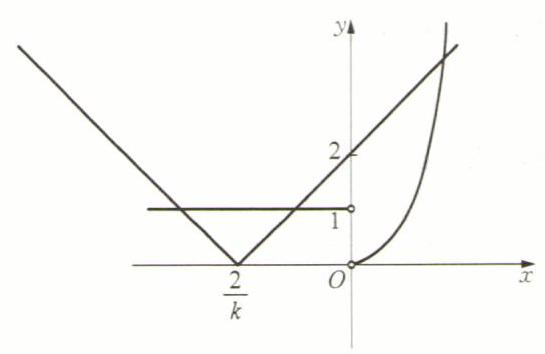
\includegraphics[max width=0.4\textwidth]{images/bo_d29ci7n7aajc738p8c80_38_295_1494_545_354_0.jpg}
\end{center}
\hspace*{3em} 

第 6 题图 1

\begin{center}
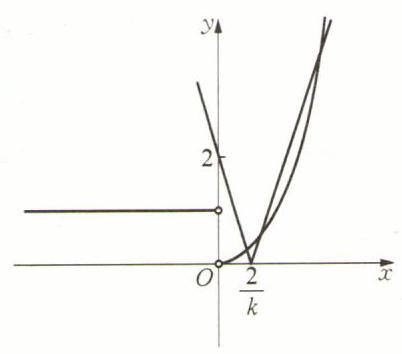
\includegraphics[max width=0.3\textwidth]{images/bo_d29ci7n7aajc738p8c80_38_963_1492_402_354_0.jpg}
\end{center}
\hspace*{3em} 

第 6 题图 2

7.【答案】 $\left( {-3 + 2\sqrt{2},0}\right)  \cup  \left( {0,1}\right)$

【解析】由函数的解析式得 $f\left( 0\right)  \neq  0$ ,而 $f\left( 1\right)  = 0$ ,所以 $x = 1$ 是函数 $f\left( x\right)$ 的一个零点.

当 $x \neq  0$ 且 $x \neq  1$ 时,只需 $f\left( x\right)  = {mx}\left| {x - 1}\right|  - \left| x\right|  + 1 = 0$ 有两个根即可,分离参数得

$m = \left\{  \begin{array}{lll} \dfrac{1}{x}, & x > 1, & \\   - \dfrac{1}{x}, & 0 < x < 1,\text{ 有两个根. 令 }h\left( x\right)  = \left\{  \begin{array}{ll} \dfrac{1}{x}, & x > 1, \\   - \dfrac{1}{x}, & 0 < x < 1,\text{ 则 }y = \\  \dfrac{x + 1}{x\left( {x - 1}\right) }, & x < 0, \end{array}\right. & \\   & \dfrac{x + 1}{x\left( {x - 1}\right) }, & x < 0, \end{array}\right.$

$h\left( x\right)$ 与 $y = m$ 有两个交点. 当 $0 < x < 1$ 和 $x > 1$ 时 $h\left( x\right)$ 的图象如图所示.

\begin{center}
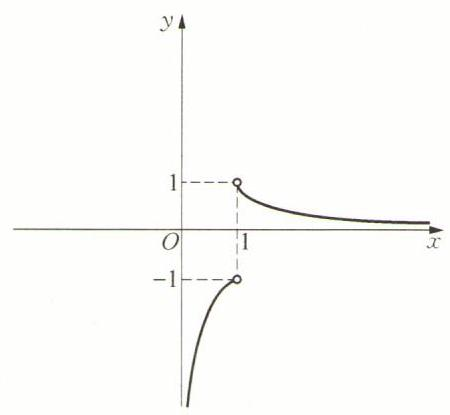
\includegraphics[max width=0.3\textwidth]{images/bo_d29ci7n7aajc738p8c80_39_1043_529_450_415_0.jpg}
\end{center}
\hspace*{3em} 

第 7 题图

易见,当 $m \in  \left( {-\infty , - 1}\right)  \cup  \left( {0,1}\right)$ 时, $y = h\left( x\right)$ 的 $0 < x < 1$ 和 $x > 1$ 部分图象与 $y = m$ 有一个交点; 当 $m \in  \left\lbrack  {-1,0}\right\rbrack   \cup  \lbrack 1, + \infty )$ ,没有交点.

下面研究方程 $m = \dfrac{x + 1}{x\left( {x - 1}\right) }\left( {x < 0}\right)$ 的根的情况,化简得 $m{x}^{2} - \left( {m + 1}\right) x - 1 = 0\left( {x < 0}\right)$ . 易知, $m = 0$ 时, 不符合题意；若该二次方程有两个不同负根,将

$\left\{  \begin{array}{l} \Delta  = {\left( m + 1\right) }^{2} + {4m} > 0, \\  \dfrac{m + 1}{m} < 0,\text{ 解得 } - 3 + 2\sqrt{2} < m < 0,\text{ 此 } \\  \dfrac{-1}{m} > 0, \end{array}\right.$

时 $0 < x < 1$ 和 $x > 1$ 部分图象没交点,故符合题意 $y = h\left( x\right)$ 与 $y = m$ 有两个交点; 若该二次方程只有一个负根,则根的情况是两个相等的负根或者一正一负根,得

$\left\{  \begin{array}{l} \Delta  = {\left( m + 1\right) }^{2} + {4m} = 0, \\  \dfrac{m + 1}{m} < 0 \end{array}\right.$ 或 $\left\{  \begin{array}{ll} \Delta  = {\left( m + 1\right) }^{2} + {4m} > 0, & \\  \dfrac{-1}{m} < 0, & \text{ 解得 }m =  - 3 + 2\sqrt{2}\text{ 或 }m > 0, \\  \dfrac{1}{m} < 0, & \text{ 此时 } \end{array}\right.$

$0 < x < 1$ 和 $x > 1$ 部分图象需要有一个交点,即 $m \in  \left( {-\infty , - 1}\right)  \cup  \left( {0,1}\right)$ ,故 $0 < m <$ 1 时 $y = h\left( x\right)$ 与 $y = m$ 有两个交点.

综上,要使函数 $y = f\left( x\right)$ 有三个零点, $m$ 的取值范围是 $- 3 + 2\sqrt{2} < m < 0$ 或 $0 < m < 1$ . 补充说明: 本题也可以根据函数的单调性与极值情况,直接作出函数 $y = \dfrac{x + 1}{x\left( {x - 1}\right) }\left( {x < 0}\right)$ 的图象.

8.【答案】[4,60]

【解析】由 $f\left( x\right)  = \left\{  \begin{array}{ll} 3\sin {2x}, & x \leq  0, \\  {2}^{x} - 3, & x > 0, \end{array}\right.$ 得 $f\left( 2\right)  = 1$ ,则 $y = \left| {f\left( x\right)  - f\left( \alpha \right) }\right|  = \left| {f\left( x\right)  - 1}\right|$ , 作出函数 $f\left( x\right)$ 的图象如图所示. 当 $- 2 \leq  m \leq   - 1$ 时, ${\left| f\left( x\right)  - 1\right| }_{\max } = \left| {\left( {-3}\right)  - 1}\right|  = 4$ ;

当 $m >  - 1$ 时, $m + 4 > 3$ , ${2}^{m + 4} - 3 - 1 = {2}^{m + 4} - 4 > 4$ . 所以当 $- 1 < m \leq  2$ 时, ${Z}_{\alpha }\left\lbrack  {m,m + 4}\right\rbrack   = {2}^{m + 4} - 4$ ,则 ${Z}_{2}\lbrack m$ , $m + 4\rbrack$ 的最大值为 ${2}^{6} - 4 = {60}$ ,即 ${Z}_{2}\left\lbrack  {m,m + 4}\right\rbrack$ 的取值范围是 $\left\lbrack  {4,{60}}\right\rbrack$ .

\begin{center}
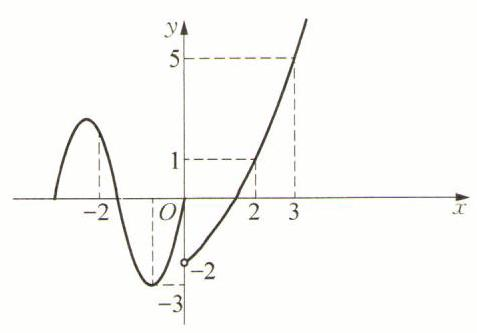
\includegraphics[max width=0.4\textwidth]{images/bo_d29ci7n7aajc738p8c80_40_1023_142_477_333_0.jpg}
\end{center}
\hspace*{3em} 

第 8 题图

9.【答案】 $\dfrac{2 + \sqrt{2}}{2}$ 或 $\dfrac{{10} - \sqrt{2}}{4}$

【解析】因为 $f\left( x\right)$ 是奇函数,且图象关于直线 $x = 1$ 对称,所以 $f\left( {x + 2}\right)  = f\left( {1 + \left( {x + 1}\right) }\right)  = f(1 - (x +$  $1)) = f\left( {-x}\right)  =  - f\left( x\right) ,f\left( {x + 4}\right)  =  - f\left( {x + 2}\right)  =$  $f\left( x\right)$ ,所以 $f\left( x\right)$ 是周期函数,4是它的一个周期. 由奇函数、周期性作出函数的图象, 如图所示.

\begin{center}
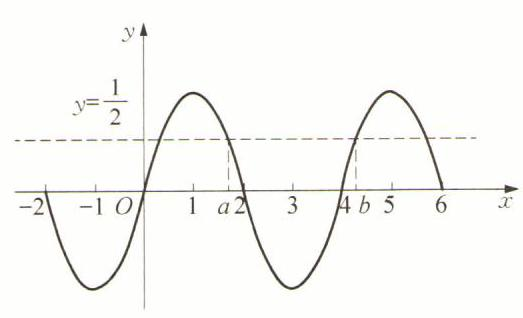
\includegraphics[max width=0.4\textwidth]{images/bo_d29ci7n7aajc738p8c80_40_974_548_523_318_0.jpg}
\end{center}
\hspace*{3em} 

第 9 题图

当 $x \in  \left\lbrack  {0,2}\right\rbrack$ 时, $f\left( x\right)  = x\left( {2 - x}\right)  =  - {\left( x - 1\right) }^{2} +$ 1,最大值为 1,因此 $f\left( x\right)$ 的最大值为 1,且 $f\left( 1\right)  = 1$ , $f\left( 5\right)  = 1$ ,由于 ${M}_{\left\lbrack  0,k\right\rbrack  } = 2{M}_{\left\lbrack  k,2k\right\rbrack  }$ ,因此 $1 \notin  \left\lbrack  {k,{2k}}\right\rbrack$ ,

则有以下两种情况:

① ${2k} < 1$ 时,则因为 $f\left( x\right)$ 在 $\left\lbrack  {0,1}\right\rbrack$ 上递增,所以 $0 < {M}_{\left\lbrack  0,k\right\rbrack  } < {M}_{\left\lbrack  k,2k\right\rbrack  },{M}_{\left\lbrack  0,k\right\rbrack  } = 2{M}_{\left\lbrack  k,2k\right\rbrack  }$ 不可能成立.

② $k > 1$ 时,此时有 $1 \in  \left\lbrack  {0,k}\right\rbrack$ ,所以 ${M}_{\left\lbrack  0,k\right\rbrack  } = 1,{M}_{\left\lbrack  k,2k\right\rbrack  } = \dfrac{1}{2}$ . 如图,设 $1 < a < 2,4 < b$  $< 5$ ,且 $f\left( a\right)  = f\left( b\right)  = \dfrac{1}{2}$ . 故有 $\left\lbrack  {k,{2k}}\right\rbrack   \subseteq  \left\lbrack  {a,b}\right\rbrack$ ,且 $k = a$ 或 ${2k} = b$ . 由 $x\left( {2 - x}\right)  = \dfrac{1}{2}$ 得 $x = 1 + \dfrac{\sqrt{2}}{2}$ 或 $x = 1 - \dfrac{\sqrt{2}}{2}$ ,所以图中 $a = 1 + \dfrac{\sqrt{2}}{2},b = 1 - \dfrac{\sqrt{2}}{2} + 4 = 5 - \dfrac{\sqrt{2}}{2}$ ,

当 $k = a = 1 + \dfrac{\sqrt{2}}{2}$ 时, ${2k} = 2 + \sqrt{2} < b$ ,满足题意,当 ${2k} = b = 5 - \dfrac{\sqrt{2}}{2}$ 时, $k = \dfrac{{10} - \sqrt{2}}{4} > a$ , 满足题意. 综上, $k$ 的值为 $\dfrac{2 + \sqrt{2}}{2}$ 或 $\dfrac{{10} - \sqrt{2}}{4}$ .

10.【答案】 $\left( {-\dfrac{1}{505},\dfrac{1}{504}}\right)$

\begin{center}
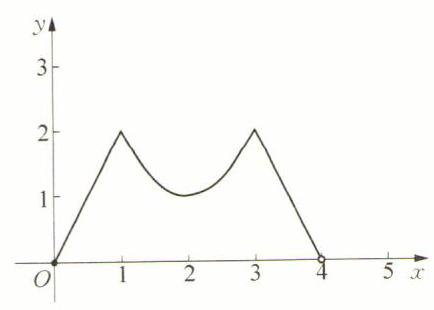
\includegraphics[max width=0.3\textwidth]{images/bo_d29ci7n7aajc738p8c80_40_1075_1754_434_310_0.jpg}
\end{center}
\hspace*{3em} 

第 10 题图

【解析】作出函数在 $x \in  \lbrack 0,4)$ 上的图象如图所示,由 $f\left( {x + 4}\right)  = f\left( x\right)  + a$ 知,函数 $f\left( x\right)$ 是以 4 为周期,且每个周期上下平移 $\left| a\right|$ 个单位的一个函数,若使 $x \in  \lbrack 0$ , 2021] 时,存在 $k \in  \mathbf{R}$ ,方程 $g\left( x\right)  = f\left( x\right)  + k$ 在 $x \in  \lbrack 0$ ,

2021] 上恰有 2021 个零点,等价于 $f\left( x\right)  =  - k$ 在 $x \in  \left\lbrack  {0,{2021}}\right\rbrack$ 上恰有 2021 个交点,如图所示,可知在每个周期都有 4 个交点,即 $- k \in  \left( {1,2}\right)$ 时满足条件,且必须每个周期内均应使 $- k$ 处在极大值和极小值之间,才能保证恰有 2021 个交点,则当 $a \geq  0$ 时,需使最后一个完整周期[2016,2020)中的极小值 $f\left( {2018}\right)  < 2$ ,即 $f\left( {2018}\right)  = f\left( 2\right)  + {504a} = 1 + {504a} <$

2,解得 $a < \dfrac{1}{504}$ ,即 $a \in  \left\lbrack  {0,\dfrac{1}{504}}\right)$ ; 当 $a < 0$ 时,需使最后一个极大值 $f\left( {2021}\right)  > 1$ ,即 $f\left( {2021}\right)  = f\left( 1\right)  + {505a} = 2 + {505a} > 1$ ,解得 $a >  - \dfrac{1}{505}$ ,即 $a \in  \left( {-\dfrac{1}{505},0}\right)$ . 综上所述, $a \in$  $\left( {-\dfrac{1}{505},\dfrac{1}{504}}\right)$ .

11.【答案】 $\lbrack  - 2,6)$

【解析】设函数 $g\left( x\right)  = \dfrac{x}{4{x}^{2} + {16}},x \geq  2$ 的值域为 $A$ ,函数 $h\left( x\right)  = {\left( \dfrac{1}{2}\right) }^{\left| x - a\right| },x < 2$ 的值域为 $B$ ,因为对任意的 ${x}_{1} \in  \lbrack 2, + \infty )$ ,都存在唯一的 ${x}_{2} \in  \left( {-\infty ,2}\right)$ ,满足 $f\left( {x}_{2}\right)  = f\left( {x}_{1}\right)$ , 则有 $A \subseteq  B$ ,且 $B$ 中若有元素与 $A$ 中元素对应,则只有一个. 易知 $A = \left( {0,\dfrac{1}{16}}\right\rbrack$ .

可知 $y = {\left( \dfrac{1}{2}\right) }^{\left| x\right| }$ 的图象如图所示, $h\left( x\right)  = {\left( \dfrac{1}{2}\right) }^{\left| x - a\right| },x < 2$ 为 $y = {\left( \dfrac{1}{2}\right) }^{\left| x\right| }$ 的图象左右平移并取 $x = 2$ 左边的部分.

① 当 $a \geq  0$ 时,相当于把 $y = {\left( \dfrac{1}{2}\right) }^{\left| x\right| }$ 的图象向右平移 $a$ 个单位,由图象可知,最多把 $C$ 点移到 $x = 2$ 处,即最多向右平移 6 个单位 (不含). 即 $0 \leq  a < 6$ 时满足题意.

\begin{center}
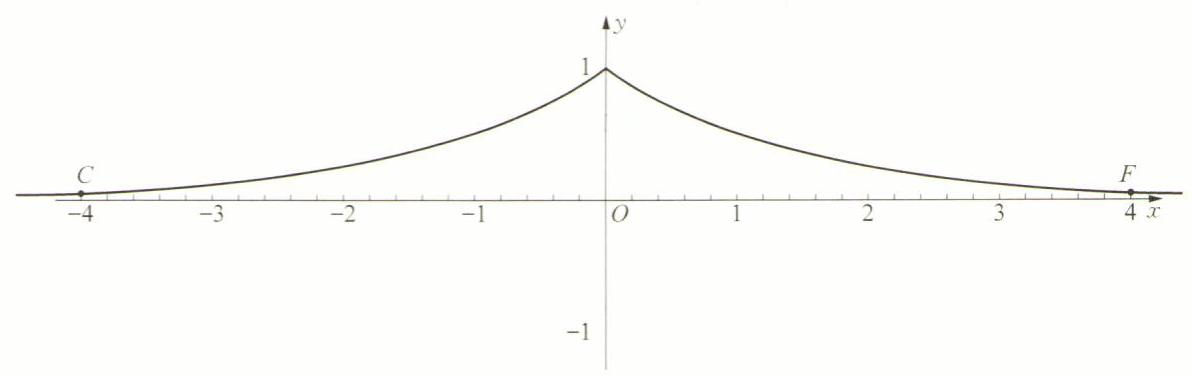
\includegraphics[max width=1.0\textwidth]{images/bo_d29ci7n7aajc738p8c80_41_220_1393_1193_377_0.jpg}
\end{center}
\hspace*{3em} 

第 11 题图

② 当 $a < 0$ 时,相当于把 $y = {\left( \dfrac{1}{2}\right) }^{\left| x\right| }$ 的图象向左平移 $- a$ 个单位,由图象可知,最多把 $F$ 点移到 $x = 2$ 处,即最多向左平移 2 个单位 (含). 即 $0 <  - a \leq  2$ 时满足题意. 综上, $- 2 \leq  a < 6$ . 13 分段函数

1.【答案】 $\left\lbrack  {\dfrac{3}{2},2}\right)$

【解析】因为 $f\left( x\right)$ 在 $\mathbf{R}$ 上单调递增,所以需要: $f\left( x\right)$ 的左支 $y = \left( {2 - a}\right) x + \dfrac{1}{2}\left( {x < 1}\right)$ 单调递增,即 $2 - a > 0;f\left( x\right)$ 的右支 $y = {\log }_{a}\left( {a{x}^{2} - x + 1}\right) \left( {x \geq  1}\right)$ 也单调递增,即

$\left\{  \begin{array}{l} a > 1, \\  \dfrac{1}{2a} \leq  1, \\  a - 1 + 1 > 0; \end{array}\right.$ 左支端点小于等于右支端点,即 ${\left. \left( 2 - a\right) x + \dfrac{1}{2}\right| }_{x = 1} \leq  {\left. {\log }_{a}\left( a{x}^{2} - x + 1\right) \right| }_{x = 1}$ . 综上, $a$ 的取值范围是 $\left\lbrack  {\dfrac{3}{2},2}\right)$ .

2.【答案】B

\begin{center}
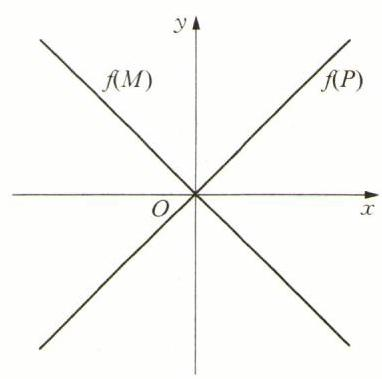
\includegraphics[max width=0.3\textwidth]{images/bo_d29ci7n7aajc738p8c80_42_1129_913_382_379_0.jpg}
\end{center}
\hspace*{3em} 

第 2 题图

【解析】由题意知函数 $f\left( P\right) ,f\left( M\right)$ 的图象如图所示.

设 $P = \lbrack 0, + \infty ),M = \left( {-\infty ,0}\right) ,f\left( P\right)  = \lbrack 0, + \infty ),f\left( M\right)  =$  $\left( {0, + \infty }\right)$ ,则 $P \cap  M = \varnothing$ ,而 $f\left( P\right)  \cap  f\left( M\right)  = \lbrack 0, + \infty ) \neq$  $\varnothing$ ,故 ①、③ 错误; 因为 $P \cap  M \neq  \varnothing$ ,必有 $P \cap  M \neq  \{ 0\}$ ,此时有 $0 \in  f\left( P\right)  \cap  f\left( M\right)$ ,故 ② 正确; 若 ${x}_{0} \notin  P \cup  M$ : 若 ${x}_{0} = 0$ , 则 $0 \notin  f\left( P\right)  \cup  f\left( M\right)$ ; 若 ${x}_{0} \neq  0$ ,则 ${x}_{0}, - {x}_{0}$ 至少有一数不属于 $f\left( P\right)  \cup  f\left( M\right)$ ,故 ④ 正确.

3.【答案】A

【解析】作出 $y = 1 - \left| {{2}^{x - 1} - 1}\right|  = \left\{  \begin{array}{ll} {2}^{x - 1}, &  - 5 \leq  x \leq  1, \\  2 - {2}^{x - 1}, & 1 < x \leq  5 \end{array}\right.$ 与 $y = {2x} - {x}^{2},x \in  \left\lbrack  {-5,5}\right\rbrack$ 的图象,如图所示. 因为两函数同时在 $x = 1$ 处取得最大值 1,所以 $f\left( 1\right)  = 1$ 必为函数 $f\left( x\right)$ 的最大值. 若 $f\left( x\right)  = \left\{  {\begin{array}{ll} 1 - \left| {{2}^{x - 1} - 1}\right| , & x \in  ( - 5,5\rbrack , \\  {2x} - {x}^{2}, & x \in  \{  - 5\} , \end{array}\text{ 则 }f\left( x\right) }\right.$ 有最小值-35; 若 $f\left( x\right)  = \left\{  \begin{array}{ll} 1 - \left| {{2}^{x - 1} - 1}\right| , & x \in  \{  - 5\} , \\  {2x} - {x}^{2}, & x \in  ( - 5,5\rbrack , \end{array}\right.$ 此时 $f\left( x\right)$ 没有最小值. 所以 $f\left( x\right)$ 有最大值,但不一定有最小值.

\begin{center}
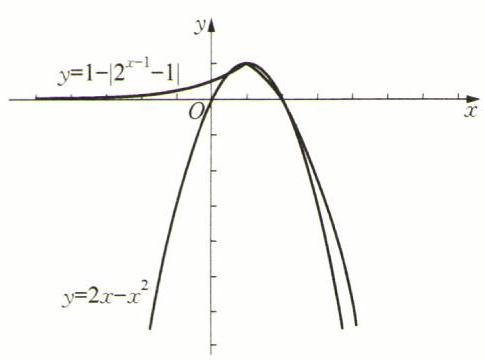
\includegraphics[max width=0.4\textwidth]{images/bo_d29ci7n7aajc738p8c80_42_1027_1632_484_360_0.jpg}
\end{center}
\hspace*{3em} 

第 3 题图

4.【答案】D

【解析】易知, ${x}_{0}$ 足够小时,函数 $f\left( x\right)$ 在 $\left( {-\infty ,{x}_{0}}\right)$ 上必严格单调递减,因为 $f\left( x\right)$ 在 $\left( {-\infty , + \infty }\right)$ 上单调,所以 $f\left( x\right)$ 在 $\left( {-\infty , + \infty }\right)$ 上必为单调递减函数. 欲使 $y =  - x \mid  x +$  ${2a} \mid  ,x <  - 1$ 单调递减,根据函数的图象,可知 $- 1 \leq   - {2a} \leq  0 \Rightarrow  0 \leq  a \leq  \dfrac{1}{2}$ ；欲使 $y = {0.5} +$  ${\log }_{a}\left( {x + 2}\right) ,x \geq   - 1$ 单调递减,可知 $0 < a < 1$ ；欲使函数 $f\left( x\right)$ 在 $\left( {-\infty , + \infty }\right)$ 上单调递减,则必须有 $1 - {2a} \geq  \dfrac{1}{2}$ ,解得 $a \leq  \dfrac{1}{4}$ . 所以 $0 < a \leq  \dfrac{1}{4}$ .

当 $x \geq   - 1$ 时, $f\left( x\right)  = \dfrac{1}{2} + {\log }_{a}\left( {x + 2}\right)  = 0$ ,可得 $x = \dfrac{1}{\sqrt{a}} - 2 \geq  0$ ,令 $\left| {{ax} - \dfrac{1}{2}}\right|  = 0$ ,可得 $x =$  $\dfrac{1}{2a}$ ,因为 $\dfrac{1}{2a} - \left( {\dfrac{1}{\sqrt{a}} - 2}\right)  = \dfrac{{4a} - 2\sqrt{a} + 1}{2a} = \dfrac{{\left( 2\sqrt{a} - \dfrac{1}{2}\right) }^{2} + \dfrac{3}{4}}{2a} > 0$ ,则 $\dfrac{1}{2a} > \dfrac{1}{\sqrt{a}} - 2$ ,则可作出 $y = \left| {f\left( x\right) }\right|$ 和 $y = \left| {{ax} - \dfrac{1}{2}}\right|$ 的草图如图所示. 因为 $0 < \dfrac{1}{2} + {\log }_{a}1 < a + \dfrac{1}{2}$ , 所以函数 $y = \left| {f\left( x\right) }\right|$ 与函数 $y =$  $\left| {{ax} - \dfrac{1}{2}}\right|$ 在[-1,+∞)上的图象有两个交点,由题意可知,只需函数 $y =$  $\left| {f\left( x\right) }\right|$ 与函数 $y = \left| {{ax} - \dfrac{1}{2}}\right|$ 在 $( - \infty$ ,

\begin{center}
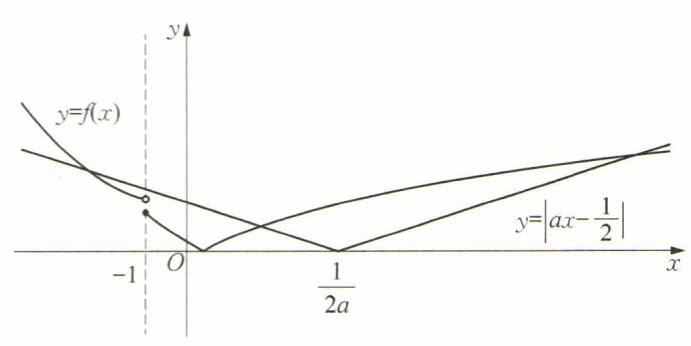
\includegraphics[max width=0.5\textwidth]{images/bo_d29ci7n7aajc738p8c80_43_798_821_691_346_0.jpg}
\end{center}
\hspace*{3em} 

第 4 题图

$- 1)$ 上的图象有且只有一个交点,联立 $\left\{  \begin{array}{l} y = {x}^{2} + {2ax}, \\  y =  - {ax} + \dfrac{1}{2}, \end{array}\right.$ 可得 ${x}^{2} + {3ax} - \dfrac{1}{2} = 0$ ,设 $h\left( x\right)  =$  ${x}^{2} + {3ax} - \dfrac{1}{2}$ ,则函数 $h\left( x\right)$ 在 $\left( {-\infty , - 1}\right)$ 上有且只有一个零点,二次函数 $h\left( x\right)$ 的对称轴方程为 $x =  - \dfrac{3a}{2} \in  \left\lbrack  {-\dfrac{3}{8},0}\right)$ ,只需 $h\left( {-1}\right)  =  - {3a} + \dfrac{1}{2} < 0$ ,解得 $a > \dfrac{1}{6}$ . 综上所述, $\dfrac{1}{6} < a \leq  \dfrac{1}{4}$ .

5.【答案】 $\left\{  {\dfrac{2}{3}, - 3 - \sqrt{13}}\right\}$

【解析】易知, $g\left( x\right)  = \left| {x + a}\right|  + \left| {x - 2}\right| ,x > 0$ 的最小值为 $A = \left| {2 + a}\right|$ . 设 $h\left( x\right)  = {x}^{2} -$  ${ax} + \dfrac{1}{2}a + 1,x \leq  0$ 的最小值为 $B$ ,分以下两种情况讨论: 当 $a \geq  0$ 时, $y = {x}^{2} - {ax} + \dfrac{1}{2}a +$

1 的对称轴 ${x}_{0} = \dfrac{a}{2}$ 大于等于 0,所以函数 $h\left( x\right)$ 在 $\left( {-\infty ,0}\right\rbrack$ 上单调递减,故 $B = \dfrac{1}{2}a + 1$ ; 当 $a < 0$ 时, $y = {x}^{2} - {ax} + \dfrac{1}{2}a + 1$ 的对称轴 ${x}_{0} = \dfrac{a}{2}$ 小于 0,所以函数 $h\left( x\right)$ 在 $( - \infty ,0\rbrack$ 上先单调递减,再单调递增,故 $B = h\left( \dfrac{a}{2}\right)  =  - \dfrac{{a}^{2}}{4} + \dfrac{1}{2}a + 1$ .

① 当 $A = \left| {2 + a}\right|  = {2a}$ 时,解得 $a = 2$ ,此时 $B = \dfrac{1}{2}a + 1 = 2 < 2 \cdot  2 = 4$ ,不符合题意.

② 当 $B = \dfrac{1}{2}a + 1 = {2a}$ 时,解得 $a = \dfrac{2}{3}$ ,此时 $a \geq  0$ 且 $A = \left| {2 + a}\right|  = \dfrac{8}{3} > 2 \cdot  \dfrac{2}{3}$ ,符合题意.

③ 当 $B =  - \dfrac{{a}^{2}}{4} + \dfrac{1}{2}a + 1 = {2a}$ 时,解得 $a =  - 3 \pm  \sqrt{13}$ (正舍),此时 $a < 0$ 且 $A = \left| {2 + a}\right|  >$  ${2a}$ ,符合题意.

综上所述,实数 $a$ 的取值集合为 $\left\{  {\dfrac{2}{3}, - 3 - \sqrt{13}}\right\}$ .

6.【答案】②

【解析】 根据初等函数的图象以及图象的平移翻折变换, 可画出 $f\left( x\right)$ 的图象,如图所示.

\begin{center}
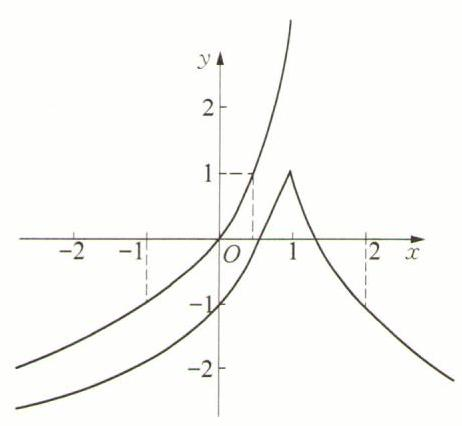
\includegraphics[max width=0.3\textwidth]{images/bo_d29ci7n7aajc738p8c80_44_1055_1039_462_426_0.jpg}
\end{center}
\hspace*{3em} 

第 6 题图

对于 ①: 当 $n = 0$ 时, $f\left( x\right)  = \left\{  \begin{array}{ll} {\log }_{\dfrac{1}{2}}\left( {1 - x}\right) , &  - 1 \leq  x \leq  0, \\  {2}^{2 - \left| {x - 1}\right| } - 3, & 0 < x \leq  m, \end{array}\right.$ 由函数图象可知: 要使 $f\left( x\right)$ 的值域是 $\left\lbrack  {-1,1}\right\rbrack$ ,则 $m \in$  $(1,2\rbrack$ ,故 ① 错误；

对于 ②: 当 $n = \dfrac{1}{2}$ 时, $f\left( x\right)  = {\log }_{\dfrac{1}{2}}\left( {1 - x}\right) ,f\left( x\right)$ 在 $\left\lbrack  {-1,\dfrac{1}{2}}\right\rbrack$ 单调递增, $f\left( x\right)$ 的最大值为 1,最小值为 -1,

则 $m \in  \left( {\dfrac{1}{2},2}\right\rbrack$ ,故 ② 正确;

对于 ③: 当 $n \in  \left\lbrack  {0,\dfrac{1}{2}}\right)$ 时, $m \in  \left\lbrack  {1,2}\right\rbrack$ ,故 ③ 错误.

7.【答案】 $\left( {-\infty , - \sqrt{2}}\right)$

【解析】易知,函数 $f\left( x\right)$ 在区间 $\left( {-\infty ,0}\right)$ 上的图象是连续的. 若存在相异的实数 ${x}_{1},{x}_{2} \in$  $\left( {-\infty ,0}\right)$ ,使得 $f\left( {x}_{1}\right)  = f\left( {x}_{2}\right)$ 成立,只需 $f\left( x\right)$ 在区间 $\left( {-\infty ,0}\right)$ 内不要是严格单调即可. 现考虑 $f\left( x\right)$ 在区间 $\left( {-\infty ,0}\right)$ 上的严格单调的情况.

易知: $f\left( x\right)  = \dfrac{1}{x} + \left| {{2x} - a}\right|  = \left\{  \begin{array}{ll} {2x} + \dfrac{1}{x} - a, & x \geq  \dfrac{a}{2}, \\  \dfrac{1}{x} - {2x} + a, & x < \dfrac{a}{2}. \end{array}\right.$

当 $a \geq  0$ 时: $x < 0$ 时, $f\left( x\right)  = \dfrac{1}{x} - {2x} + a$ ,显然 $f\left( x\right)$ 在 $\left( {-\infty ,0}\right)$ 单调递减;

当 $a < 0$ 时: $x < \dfrac{a}{2}$ 时, $f\left( x\right)  = \dfrac{1}{x} - {2x} + a$ ,显然 $f\left( x\right)$ 在 $\left( {-\infty ,\dfrac{a}{2}}\right)$ 单调递减,欲使 $f\left( x\right)$ 在区间 $\left( {-\infty ,0}\right)$ 上严格单调,需使 $f\left( x\right)  = {2x} + \dfrac{1}{x} - a$ 在 $\left\lbrack  {\dfrac{a}{2},0}\right)$ 上也严格单调递减,且 ${\left. \left( \dfrac{1}{x} - 2x + a\right) \right| }_{x = \dfrac{a}{2}} \geq  {\left. \left( 2x + \dfrac{1}{x} - a\right) \right| }_{x = \dfrac{a}{2}}$ ,解得 $- \sqrt{2} \leq  a < 0$ . 可知,当 $a \geq   - \sqrt{2}$ 时, $f\left( x\right)$ 在区间 $\left( {-\infty ,0}\right)$ 上严格单调,此时不存在相异的实数 ${x}_{1},{x}_{2} \in  \left( {-\infty ,0}\right)$ ,使得 $f\left( {x}_{1}\right)  =$  $f\left( {x}_{2}\right)$ 成立. 所以,若存在相异的实数 ${x}_{1},{x}_{2} \in  \left( {-\infty ,0}\right)$ ,使得 $f\left( {x}_{1}\right)  = f\left( {x}_{2}\right)$ 成立时,须有 $a <  - \sqrt{2}$ .

\section*{14 复合函数的零点问题}

1.【答案】 ${C}$

【解析】由函数 $f\left( x\right)$ 是定义域为 $\mathbf{R}$ 的偶函数,故图象关于 $y$ 轴对称,作出 $f\left( x\right)$ 的图象如图所示. 令 $f\left( x\right)  = t$ ,则原方程可化为 $m \cdot  {t}^{2} + n \cdot  t + 1 = 0$ , 根据图象可知,原方程恰好有 7 个不同的实数根,只需 $m \cdot  {t}^{2} + n \cdot  t + 1 = 0$ 有两个不等的实数根 $\dfrac{1}{2}\text{ 、 }\dfrac{3}{2}$ , 由韦达定理得 $\dfrac{1}{2} + \dfrac{3}{2} =  - \dfrac{n}{m},\dfrac{1}{2} \times  \dfrac{3}{2} = \dfrac{1}{m}$ ,解得 $m =$  $\dfrac{4}{3},n =  - \dfrac{8}{3}$ ,于是 $m - n = 4$ .

\begin{center}
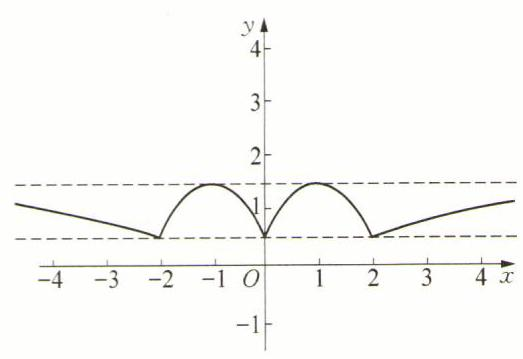
\includegraphics[max width=0.4\textwidth]{images/bo_d29ci7n7aajc738p8c80_45_971_1124_523_359_0.jpg}
\end{center}
\hspace*{3em} 

第 1 题图

2.【答案】 $\left( {\dfrac{8}{5},4}\right)$

\begin{center}
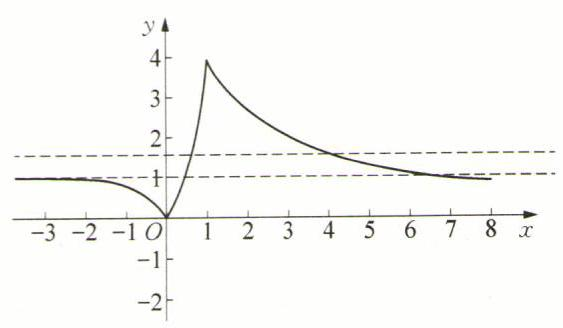
\includegraphics[max width=0.4\textwidth]{images/bo_d29ci7n7aajc738p8c80_45_937_1728_563_328_0.jpg}
\end{center}
\hspace*{3em} 

第 2 题图

【解析】作出函数 $f\left( x\right)$ 的图象如图所示. 设 $t =$  $f\left( x\right)$ ,则 $f\left( t\right)  = a$ 恰有 5 个不同的实数根,当 $a <$ 0时, $f\left( t\right)  = a$ 无解,不符合题意,当 $a = 0$ 时, $f\left( t\right)  = a$ 有唯一解, $t = 0$ ,此时, $f\left( x\right)  = t = 0$ ,解得 $x = 0$ 有一解,不符合题意,当 $0 < a < 1$ 时, $f\left( t\right)  =$  $a$ 有三解, ${t}_{1} < 0,0 < {t}_{2} < 1,{t}_{3} > 7$ ,此时, $f\left( x\right)  = {t}_{1}$ 无解, $f\left( x\right)  = {t}_{2}$ 有三解, $f\left( x\right)  = {t}_{3}$ 无解,共三解,不符合题意; 当 $a = 1$ 时, $f\left( t\right)  = a$ 有两解, ${t}_{4} = {\log }_{5}2,{t}_{5} = 7$ ,此时, $f\left( x\right)  = {t}_{4}$ 有三解, $f\left( x\right)  = {t}_{5}$ 无解,共三解,不符合题意; 当 $1 < a \leq  \dfrac{8}{5}$ 时, $f\left( t\right)  = a$ 有两解, ${\log }_{5}2 < {t}_{6}$  $< 1,4 \leq  {t}_{7} < 7$ ,此时, $f\left( x\right)  = {t}_{6}$ 有三解, $f\left( x\right)  = {t}_{7}$ 有一解,共四解,不符合题意; 当 $\dfrac{8}{5} <$  $a < 4$ 时, $f\left( t\right)  = a$ 有两解, ${\log }_{5}2 < {t}_{8} < 1,1 < {t}_{9} < 4$ ,此时, $f\left( x\right)  = {t}_{8}$ 有三解, $f\left( x\right)  = {t}_{9}$ 有两解,共五解,符合题意; 当 $a = 4$ 时, $f\left( t\right)  = a$ 有唯一解, $t = 1$ ,此时, $f\left( x\right)  = 1$ 有两解,不符合题意; 当 $a > 4$ 时, $f\left( t\right)  = a$ 无解,不符合题意. 综上: 实数 $a$ 的取值范围是 $\left( {\dfrac{8}{5},4}\right)$ .

3.【答案】 $\dfrac{1}{2} < k < \dfrac{9}{16}$

【解析】设 $t = {x}^{2} - 1,t \geq   - 1$ ,则 $y = {t}^{2} - \dfrac{3}{2}\left| t\right|  + k =$ 0 时, $- k = {t}^{2} - \dfrac{3}{2}\left| t\right|$ ,设 $g\left( t\right)  = {t}^{2} - \dfrac{3}{2}\left| t\right| ,t \geq$ -1,则 $g\left( t\right)  = {t}^{2} - \dfrac{3}{2}\left| t\right|  = \left\{  \begin{array}{ll} {t}^{2} - \dfrac{3}{2}t, & t \geq  0, \\  {t}^{2} + \dfrac{3}{2}t, &  - 1 \leq  t < 0. \end{array}\right.$ 函数 $g\left( t\right)$ 的图象如图所示, $g\left( {-1}\right)  =  - \dfrac{1}{2},g\left( \dfrac{3}{4}\right)  = g\left( {-\dfrac{3}{4}}\right)  =  - \dfrac{9}{16}$ . 当 $- \dfrac{9}{16} <  - k \leq   - \dfrac{1}{2}$ 时, $y =  - k$ 与 $y = g\left( t\right)$ 有 4 个交点,此时两者的交点最多,设交点横坐标为 ${t}_{1} < {t}_{2} < {t}_{3} < {t}_{4}$ ,由图可知 $- 1 \leq  {t}_{1} <  - \dfrac{3}{4}, - \dfrac{3}{4} < {t}_{2} <  - \dfrac{1}{2},\dfrac{1}{2} < {t}_{3} < \dfrac{3}{4},\dfrac{3}{4}$  $< {t}_{4} \leq  1$ ,又 $t = {x}^{2} - 1$ ,若 $t =  - 1$ ,有一个解, $t >  - 1$ ,有两个解,所以当 $y =  - k$ 与 $y = g\left( t\right)$ 有 4 个交点,且交点横坐标均大于 -1 时,函数 $f\left( x\right)$ 的零点最多,所以 $- \dfrac{9}{16} <  - k <  - \dfrac{1}{2}$ , 即 $\dfrac{1}{2} < k < \dfrac{9}{16}$ .

\begin{center}
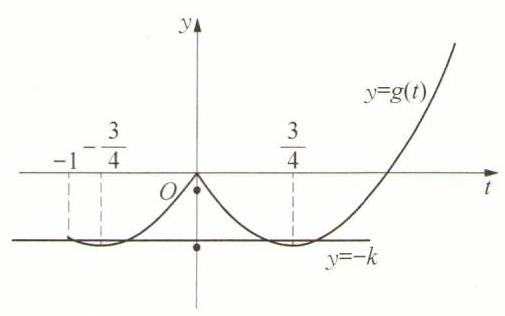
\includegraphics[max width=0.4\textwidth]{images/bo_d29ci7n7aajc738p8c80_46_1006_787_505_316_0.jpg}
\end{center}
\hspace*{3em} 

第 3 题图

4.【答案】①②

【解析】由 $y = f\left( {f\left( x\right) }\right)  - \dfrac{1}{2} = 0$ ,可得 $f\left\lbrack  {f\left( x\right) }\right\rbrack   = \dfrac{1}{2}$ .

设 $f\left( x\right)  = t$ ,则方程 $f\left( {f\left( x\right) }\right)  = \dfrac{1}{2}$ 等价于 $f\left( t\right)  = \dfrac{1}{2}$ .

若 $k > 0$ ,作出函数 $f\left( x\right)$ 的图象如图 1 所示,此时方程 $f\left( t\right)  = \dfrac{1}{2}$ 有两根,其中 ${t}_{1} > 1,{t}_{2} <$ 0. 由 $f\left( x\right)  = {t}_{1} > 1$ 有一解,由 $f\left( x\right)  = {t}_{2} < 0$ 有两解,此时共有 3 个解,即函数 $y =$  $f\left( {f\left( x\right) }\right)  - \dfrac{1}{2}$ 有 3 个零点. 所以当 $k > 0$ 时,有 3 个零点. 故 ① 正确,③ 错误.

当 $k < 0$ 时,作出函数 $f\left( x\right)$ 的图象如图 2 所示,此时方程 $f\left( t\right)  = \dfrac{1}{2}$ 有一根 ${t}_{3} > 1$ ,由 $f\left( x\right)  =$  ${t}_{3} > 1$ 有两解,即函数 $y = f\left( {f\left( x\right) }\right)  - \dfrac{1}{2}$ 有 2 个零点,所以当 $k < 0$ 时,有 2 个零点. 故 ② 正确, ④ 错误.

\begin{center}
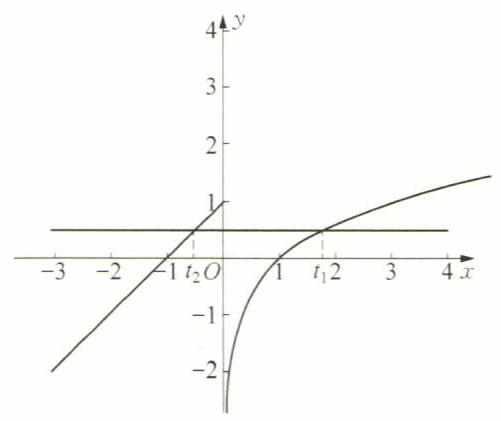
\includegraphics[max width=0.4\textwidth]{images/bo_d29ci7n7aajc738p8c80_47_290_648_501_421_0.jpg}
\end{center}
\hspace*{3em} 

第 4 题图 1

\begin{center}
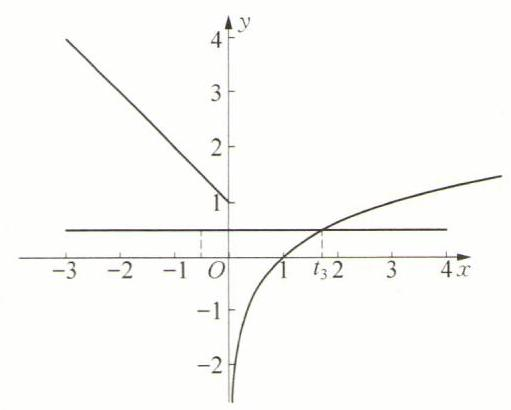
\includegraphics[max width=0.4\textwidth]{images/bo_d29ci7n7aajc738p8c80_47_843_657_511_410_0.jpg}
\end{center}
\hspace*{3em} 

第 4 题图 2

5.【答案】AC

【解析】 $f\left( x\right)  = \left\{  \begin{array}{ll} {{e}}^{x} - 2, & x \leq  0, \\  \ln x, & x > 0, \end{array}\right.$ 则由 $f\left( t\right)  + 1 = 0$ ,解得 $t = 0$ 或 $t = \dfrac{1}{{e}}$ ,则由 $f(f\left( {kx}\right)  +$  $1) + 1 = 0$ ,可得 $f\left( {kx}\right)  + 1 = 0$ 或 $f\left( {kx}\right)  + 1 = \dfrac{1}{{e}}$ ,即 $f\left( {kx}\right)  =  - 1$ 或 $f\left( {kx}\right)  = \dfrac{1}{{e}} - 1$ ,则 ① $\left\{  \begin{array}{l} {kx} \leq  0, \\  {{e}}^{kx} - 2 =  - 1, \end{array}\right.$ 或 ② $\left\{  \begin{array}{l} {kx} > 0, \\  \ln \left( {kx}\right)  =  - 1, \end{array}\right.$ 或 ③ $\left\{  \begin{array}{l} {kx} \leq  0, \\  {{e}}^{kx} - 2 = \dfrac{1}{{e}} - 1, \end{array}\right.$ 或 ④ $\left\{  \begin{array}{l} {kx} > 0, \\  \ln \left( {kx}\right)  = \dfrac{1}{{e}} - 1. \end{array}\right.$

由 ① 得 $x = 0$ ,由 ② 得 $x = \dfrac{1}{k{e}}$ ,由 ③ 得 $x \in  \varnothing$ ,由 ④ 得 $x = \dfrac{1}{k}{{e}}^{\dfrac{1}{{e}} - 1}$ .

综上,不管 $k > 0$ 还是 $k < 0$ ,函数都是 3 个零点.

\section*{15 函数新概念}

1.【答案】-4

【解析】因为 $- 1 \leq  x \leq  0$ ,所以

① 当 $x =  - 1$ 时, ${2x} =  - 2$ ,则 $\langle x\rangle  =  - 1,\langle {2x}\rangle  =  - 2$ ,得 $\langle x\rangle  + \langle {2x}\rangle  =  - 3$ ；

$f\left( \dfrac{{x}_{1} + {x}_{2}}{2}\right)  = \dfrac{f\left( {x}_{1}\right)  + f\left( {x}_{2}\right) }{2}$ ,③ 正确.

综上 ①③ 正确.

5.【答案】 -1

【解析】令 $m = n = 0$ ,则 $f\left( 1\right)  - f\left( 0\right) f\left( 0\right)  = 2 - f\left( 0\right)  - 0$ 成立,因为 $f\left( 0\right)  = 1$ ,所以 $f\left( 1\right)$  $= 2$ ,令 $m = x,n = 0$ ,则有 $f\left( 1\right)  - f\left( x\right) f\left( 0\right)  = 2 - f\left( 0\right)  - x$ ,从而有 $f\left( x\right)  = x + 1$ ,因为 ${\log }_{\dfrac{1}{2}}\left( {x + y}\right)  - {\log }_{4}x =  - {\log }_{2}\left\lbrack  {\left( {x + y}\right) \sqrt{x}}\right\rbrack$ ,所以 ${\log }_{\dfrac{1}{2}}\left( {x + y}\right)  - {\log }_{4}x$ 的最大值,即 $\left( {x + y}\right) \sqrt{x}$ 的最小值. 又因为正数 $x,y$ 使得点 $\left( {{x}^{2} - 1,3 - {2xy}}\right)$ 在函数 $y = f\left( x\right)$ 的图象上,所以有 ${x}^{2} - 1 + 1 = 3 - {2xy} \Rightarrow  y = \dfrac{3 - {x}^{2}}{2x} > 0 \Rightarrow  0 < x < \sqrt{3}$ ,所以 $\left( {x + y}\right) \sqrt{x} =$  $\left( {x + \dfrac{3 - {x}^{2}}{2x}}\right) \sqrt{x} = \dfrac{{x}^{2} + 3}{2\sqrt{x}}$ ,令 $\sqrt{x} = t \in  \left( {0,{3}^{\dfrac{1}{4}}}\right)$ ,则 $\dfrac{{x}^{2} + 3}{2\sqrt{x}} = \dfrac{{t}^{4} + 3}{2t}$ ,令 $h\left( t\right)  = \dfrac{{t}^{4} + 3}{2t}$ ,则 ${h}^{\prime }\left( t\right)  = \dfrac{3\left( {{t}^{4} - 1}\right) }{2{t}^{2}} = \dfrac{3\left( {{t}^{2} + 1}\right) \left( {t + 1}\right) \left( {t - 1}\right) }{2{t}^{2}}$ ,当 ${h}^{\prime }\left( t\right)  > 0 \Rightarrow  1 < t < {3}^{\dfrac{1}{4}},{h}^{\prime }\left( t\right)  < 0 \Rightarrow  0 <$  $t < 1$ ,所以函数 $h\left( t\right)$ 在(0,1)上单调递减,在 $\left( {1,{3}^{\dfrac{1}{4}}}\right)$ 上单调递增,所以 $h{\left( t\right) }_{\min } = h\left( 1\right)  =$  $\dfrac{1 + 3}{2} = 2$ ,所以 ${\left\lbrack  \left( x + y\right) \sqrt{x}\right\rbrack  }_{\min } = 2$ ,所以 ${\log }_{\dfrac{1}{2}}\left( {x + y}\right)  - {\log }_{4}x =  - {\log }_{2}\left\lbrack  {\left( {x + y}\right) \sqrt{x}}\right\rbrack   \leq$  $- {\log }_{2}2 =  - 1$ . 所以 ${\log }_{\dfrac{1}{2}}\left( {x + y}\right)  - {\log }_{4}x$ 的最大值为 -1 .

6.【答案】D

【解析】 $f\left( x\right)  = {x}^{2}$ 在 $\lbrack 1, + \infty )$ 上的值域为 $\lbrack 1, + \infty )$ . 若对任意 $k > M$ ,存在 ${x}_{1} < {x}_{2}$ ,使得 $f\left( {x}_{1}\right)  = g\left( {x}_{2}\right)  = k$ 成立,可直接作图,只需任意 $k \geq  1$ ,直线 $y = k$ 与 $f\left( x\right)  = {x}^{2}$ 和 $g\left( x\right)$ 的图象先后依次至少一个交点即可.

7.【答案】 $\sqrt{2\sqrt{2} + 2}$

【解析】先作出函数 $g\left( x\right)  = \left| {{\log }_{2}x - 1}\right|$ 的图象. 因为 $f\left( {x}_{1}^{2}\right)  = f\left( {x}_{2}^{2}\right)  = {2f}\left( {{x}_{1} + {x}_{2}}\right)$ ,由图象有 $0 < {x}_{1}^{2} < 2 < {x}_{2}^{2}$ ,又因为 $\left| {{\log }_{2}{x}_{1}^{2} - 1}\right|  = \left| {{\log }_{2}{x}_{2}^{2} - 1}\right|$ ,所以 $1 - {\log }_{2}{x}_{1}^{2} = {\log }_{2}{x}_{2}^{2} -$ 1,故 ${\log }_{2}\left( {{x}_{1}^{2}{x}_{2}^{2}}\right)  = 2$ ,所以 ${x}_{1}^{2}{x}_{2}^{2} = 4 \Rightarrow  {x}_{1}{x}_{2} = 2$ (因为题干中有 $f\left( {{x}_{1} + {x}_{2}}\right)$ ,故 ${x}_{1},{x}_{2}$ 只能同为正数). 又 ${x}_{1} + {x}_{2} \geq  2\sqrt{{x}_{1}{x}_{2}} = 2\sqrt{2}$ ,所以 ${2f}\left( {{x}_{1} + {x}_{2}}\right)  = f\left( {x}_{1}^{2}\right)  \Rightarrow  {\log }_{2}{\left( {x}_{1} + {x}_{2}\right) }^{2} -$  $2 = 1 - {\log }_{2}{x}_{1}^{2} \Rightarrow  {\log }_{2}\left( {{x}_{1}^{2} + \dfrac{4}{{x}_{1}^{2}} + 4}\right)  - 2 = 1 - {\log }_{2}{x}_{1}^{2}$ ,所以 ${x}_{1}^{4} + 4{x}_{1}^{2} + 4 = 8$ ,所以 ${x}_{1} =$  $\sqrt{2\sqrt{2} - 2}$ ,故 ${x}_{2} = \sqrt{2\sqrt{2} + 2}$ ,所以 $a \geq  \sqrt{2\sqrt{2} + 2}$ ,则实数 $a$ 的最小值为 $\sqrt{2\sqrt{2} + 2}$ .

② 当 $- 1 < x \leq  0$ 时, $- 2 < {2x} \leq  0$ ,则 $\langle x\rangle  = 0,\langle {2x}\rangle  =  - 1$ 或 0,得 $\langle x\rangle  + \langle {2x}\rangle  =  - 1$ 或 0. 所以 $A = \{  - 3, - 1,0\} ,A$ 中所有元素和为 -4 .

2.【答案】 $\left( {\dfrac{4}{3},\dfrac{5}{3}}\right\rbrack$

【解析】因为 $f\left( {{3x} + f\left( x\right) }\right)  = f\left( {6.5}\right)$ ,所以 $f\left( {{3x} + f\left( x\right) }\right)  = 7$ ,得 $6 < {3x} + f\left( x\right)  \leq  7$ , 进而得 $6 - {3x} < f\left( x\right)  \leq  7 - {3x}$ .

当 $0 < x \leq  1$ 时, $f\left( x\right)  = 1,6 - {3x} > 2$ ,不符合题意; 当 $x \geq  2$ 时, $f\left( x\right)  \geq  2,7 - {3x} \leq$ 1,不符合题意; 当 $1 < x < 2$ 时, $f\left( x\right)  = 2$ ,得 $6 - {3x} < 2 \leq  7 - {3x}$ ,解得 $\dfrac{4}{3} < x \leq  \dfrac{5}{3}$ .

3.【答案】 ${C}$

【解析】对于 ①,当 ${x}_{1} = 2$ 时, $f\left( {x}_{1}\right)  = 0$ ,此时不存在 ${x}_{2}$ ,使得 $f\left( {x}_{1}\right) f\left( {x}_{2}\right)  = 1$ ,故 ① 不是 “ $F$ 函数”；对于②,任意 ${x}_{1}$ ,都存在唯一的 ${x}_{2} =  - {x}_{1} - 2$ ,使得 $f\left( {x}_{1}\right) f\left( {x}_{2}\right)  = {{e}}^{{x}_{1} + 1}{{e}}^{-{x}_{1} - 1} =$  ${{e}}^{0} = 1$ ,故 $f\left( x\right)  = {{e}}^{x + 1}$ 是 “ $F$ 函数”; 对于 ③,对于任意 $x$ ,都有 $f\left( x\right)  = {x}^{2} + 1 \geq  1$ ,取 ${x}_{1} =$ 2,则 $f\left( {x}_{1}\right)  = 5$ ,定义域内不存在 ${x}_{2}$ ,使得 $f\left( {x}_{2}\right)  = \dfrac{1}{5}$ ,即不能使得 $f\left( {x}_{1}\right) f\left( {x}_{2}\right)  = 1$ ,故 ③ 不是 “ $F$ 函数”；对于 ④,任意 ${x}_{1} \in  \left( {0,\dfrac{\pi }{2}}\right)$ ,都存在唯一 ${x}_{2} = \dfrac{\pi }{2} - {x}_{1},{x}_{2} \in  \left( {0,\dfrac{\pi }{2}}\right)$ ,使得 $f\left( {x}_{1}\right) f\left( {x}_{2}\right)  = \tan {x}_{1} \times  \tan \left( {\dfrac{\pi }{2} - {x}_{1}}\right)  = 1$ ,故 ④ 为 “ $F$ 函数”.

4.【答案】 ${C}$

【解析】任取两个不等实数 ${x}_{1},{x}_{2} \in  \mathbf{R}$ .

① 当 ${x}_{1}$ 、 ${x}_{2}$ 均不为 0 且 ${x}_{1} + {x}_{2} = 0$ 时, $f\left( \dfrac{{x}_{1} + {x}_{2}}{2}\right)  = 0,\dfrac{f\left( {x}_{1}\right)  + f\left( {x}_{2}\right) }{2} = \dfrac{\dfrac{1}{{x}_{1}} + \dfrac{1}{{x}_{2}}}{2} =$  $\dfrac{{x}_{1} + {x}_{2}}{2{x}_{1}{x}_{2}} = 0$ ,即存在 ${x}_{1},{x}_{2} \in  \mathbf{R}$ 有 $f\left( \dfrac{{x}_{1} + {x}_{2}}{2}\right)  = \dfrac{f\left( {x}_{1}\right)  + f\left( {x}_{2}\right) }{2}$ ,① 正确;

② $f\left( \dfrac{{x}_{1} + {x}_{2}}{2}\right)  = {\left( \dfrac{{x}_{1} + {x}_{2}}{2}\right) }^{2} = \dfrac{{x}_{1}^{2} + {x}_{2}^{2} + 2{x}_{1}{x}_{2}}{4},\dfrac{f\left( {x}_{1}\right)  + f\left( {x}_{2}\right) }{2} = \dfrac{{x}_{1}^{2} + {x}_{2}^{2}}{2}$ ,令 $\dfrac{{x}_{1}^{2} + {x}_{2}^{2}}{2} = \dfrac{{x}_{1}^{2} + {x}_{2}^{2} + 2{x}_{1}{x}_{2}}{4}$ ,解得 ${x}_{1} = {x}_{2}$ ,与题目矛盾,② 错误;

③ 当 ${x}_{1} + {x}_{2} = 0$ 时, $f\left( \dfrac{{x}_{1} + {x}_{2}}{2}\right)  = \left| {{\left( \dfrac{{x}_{1} + {x}_{2}}{2}\right) }^{2} - 1}\right|  = 1,\dfrac{f\left( {x}_{1}\right)  + f\left( {x}_{2}\right) }{2} =$  $\dfrac{\left| {{x}_{1}^{2} - 1}\right|  + \left| {{x}_{2}^{2} - 1}\right| }{2}$ ,不妨令 $\left| {{x}^{2} - 1}\right|  = 1$ 可得 $x =  \pm  \sqrt{2}$ ,故存在不等 ${x}_{1},{x}_{2} \in  \mathbf{R}$ 有

\begin{center}
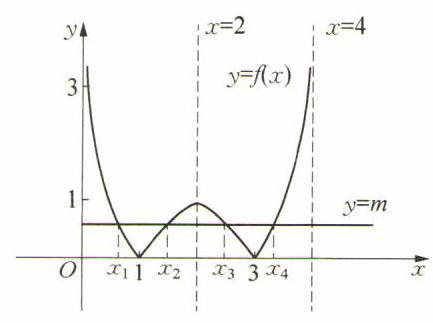
\includegraphics[max width=0.3\textwidth]{images/bo_d29ci7n7aajc738p8c80_50_1074_230_433_323_0.jpg}
\end{center}
\hspace*{3em} 

第 1 题图

1.【答案】 $\left( {{20},\dfrac{41}{2}}\right)$

【解析】当 $2 < x < 4$ 时, $f\left( x\right)  = f\left( {4 - x}\right)$ ,所以 $f\left( x\right)$ 在 (2,4)与(0,2)上的图象关于 $x = 2$ 对称.

作出图象如图所示,不妨令 ${x}_{1} < {x}_{2} < {x}_{3} < {x}_{4}$ ,显然有 $0 < {x}_{1} < 1 < {x}_{2} < 2 < {x}_{3} < 3 < {x}_{4} < 4.$

根据对称性有: ${x}_{1} + {x}_{4} = {x}_{2} + {x}_{3} = 4$ ,且因为 $f\left( {x}_{1}\right)  = f\left( {x}_{2}\right)  \Rightarrow  \left| {\ln {x}_{1}}\right|  = \left| {\ln {x}_{2}}\right|  \Rightarrow$  $- \ln {x}_{1} = \ln {x}_{2}$ ,所以 ${x}_{1}{x}_{2} = 1,{x}_{1} = \dfrac{1}{{x}_{2}},{x}_{3} = 4 - {x}_{2},{x}_{4} = 4 - {x}_{1} = 4 - \dfrac{1}{{x}_{2}}$ ,所以 ${x}_{1}^{2} + {x}_{2}^{2} +$  ${x}_{3}^{2} + {x}_{4}^{2} = \dfrac{1}{{x}_{2}^{2}} + {x}_{2}^{2} + {\left( 4 - {x}_{2}\right) }^{2} + {\left( 4 - \dfrac{1}{{x}_{2}}\right) }^{2} = 2{\left( {x}_{2} + \dfrac{1}{{x}_{2}}\right) }^{2} - 8\left( {{x}_{2} + \dfrac{1}{{x}_{2}}}\right)  + {28}$ . 因为 ${x}_{2} \in$ (1,2),令 $t = {x}_{2} + \dfrac{1}{{x}_{2}} \in  \left( {2,\dfrac{5}{2}}\right)$ ,则原式化为 $h\left( t\right)  = 2{t}^{2} - {8t} + {28},t \in  \left( {2,\dfrac{5}{2}}\right)$ . 易求得 ${20} < h\left( t\right)  < \dfrac{41}{2}$ ,所以 ${x}_{1}^{2} + {x}_{2}^{2} + {x}_{3}^{2} + {x}_{4}^{2}$ 的取值范围是 $\left( {{20},\dfrac{41}{2}}\right)$ .

2.【答案】2

【解析】不妨设 $a > 1$ . 先画出 $f\left( x\right)$ 的图象如图所示,

\begin{center}
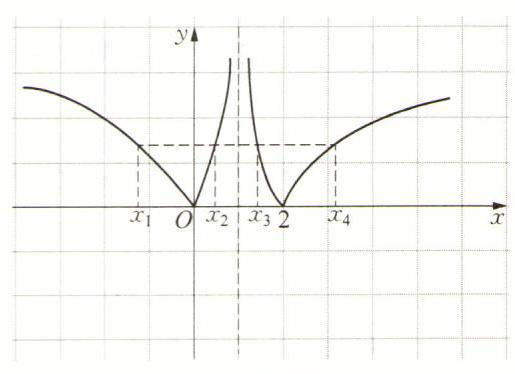
\includegraphics[max width=0.4\textwidth]{images/bo_d29ci7n7aajc738p8c80_50_991_1216_515_374_0.jpg}
\end{center}
\hspace*{3em} 

第 2 题图

易知 ${x}_{1} < 0 < {x}_{2} < 1 < {x}_{3} < 2 < {x}_{4}$ .

因为 $f\left( {x}_{1}\right)  = f\left( {x}_{2}\right)  = f\left( {x}_{3}\right)  = f\left( {x}_{4}\right)$ ,所以 $\left| {{\log }_{a}\left| {{x}_{1} - 1}\right| }\right|  = \left| {{\log }_{a}\left| {{x}_{2} - 1}\right| }\right|  = \left| {{\log }_{a}\left| {{x}_{3} - 1}\right| }\right|  =$  $\left| {{\log }_{a}\left| {{x}_{4} - 1}\right| }\right|  \Rightarrow  {\log }_{a}\left( {1 - {x}_{1}}\right)  =  - {\log }_{a}(1 -$  $\left. {x}_{2}\right)  =  - {\log }_{a}\left( {{x}_{3} - 1}\right)  = {\log }_{a}\left( {{x}_{4} - 1}\right)  \Rightarrow  {\log }_{a}\left( {1 - {x}_{1}}\right)  =$  ${\log }_{a}\dfrac{1}{1 - {x}_{2}} = {\log }_{a}\dfrac{1}{{x}_{3} - 1} = {\log }_{a}\left( {{x}_{4} - 1}\right)  \Rightarrow  1 - {x}_{1} =$  $\dfrac{1}{1 - {x}_{2}} = \dfrac{1}{{x}_{3} - 1} = {x}_{4} - 1 \Rightarrow  \left\{  {\begin{array}{l} \left( {1 - {x}_{1}}\right) \left( {1 - {x}_{2}}\right)  = 1, \\  \left( {{x}_{3} - 1}\right) \left( {{x}_{4} - 1}\right)  = 1 \end{array} \Rightarrow  }\right.$

$\left\{  {\begin{array}{l} 1 - {x}_{1} - {x}_{2} + {x}_{1}{x}_{2} = 1, \\  {x}_{3}{x}_{4} - {x}_{3} - {x}_{4} + 1 = 1 \end{array} \Rightarrow  \left\{  {\begin{array}{l} {x}_{1} + {x}_{2} = {x}_{1}{x}_{2}, \\  {x}_{3}{x}_{4} = {x}_{3} + {x}_{4} \end{array} \Rightarrow  \left\{  {\begin{array}{l} \dfrac{1}{{x}_{1}} + \dfrac{1}{{x}_{2}} = 1, \\  \dfrac{1}{{x}_{3}} + \dfrac{1}{{x}_{4}} = 1 \end{array} \Rightarrow  \dfrac{1}{{x}_{1}} + \dfrac{1}{{x}_{2}} + \dfrac{1}{{x}_{3}} + \dfrac{1}{{x}_{4}} = 2.}\right. }\right. }\right.$

3.【答案】A

【解析】先画出 $f\left( x\right)$ 的图象如图所示.

由图知: $0 < a < 1$ 时 $f\left( x\right)  = a$ 有四个实数根,且 1 $< {x}_{1} < 2 < {x}_{2} < 3 < {x}_{3} < 4 < {x}_{4} < 5$ ,又 ${x}_{3} +$  ${x}_{4} = 8$ ,由对数函数的性质: $\left( {{x}_{1} - 1}\right) \left( {{x}_{2} - 1}\right)  =$  ${x}_{1}{x}_{2} - \left( {{x}_{1} + {x}_{2}}\right)  + 1 = 1$ ,可得 $\dfrac{1}{{x}_{2}} = 1 - \dfrac{1}{{x}_{1}}$ ,所以 $\dfrac{1}{4}\left( {{x}_{3} + {x}_{4}}\right) {x}_{1} + \dfrac{1}{{x}_{2}} = 2{x}_{1} + \dfrac{1}{{x}_{2}} = 2{x}_{1} - \dfrac{1}{{x}_{1}} + 1$ ,因为 $\dfrac{3}{2} < {x}_{1} < 2$ ,所以 $\dfrac{1}{4}\left( {{x}_{3} + {x}_{4}}\right) {x}_{1} + \dfrac{1}{{x}_{2}} = 2{x}_{1} - \dfrac{1}{{x}_{1}} + 1 \in  \left( {\dfrac{10}{3},\dfrac{9}{2}}\right)$ .

\begin{center}
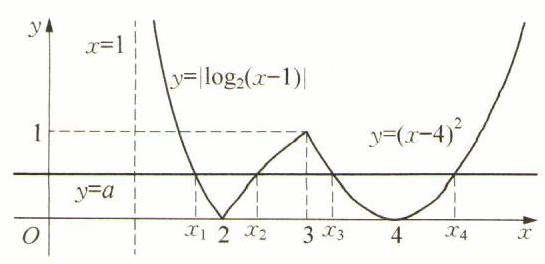
\includegraphics[max width=0.4\textwidth]{images/bo_d29ci7n7aajc738p8c80_51_962_135_545_264_0.jpg}
\end{center}
\hspace*{3em} 

第 3 题图

4.【答案】 $\dfrac{4\pi }{3}$

\begin{center}
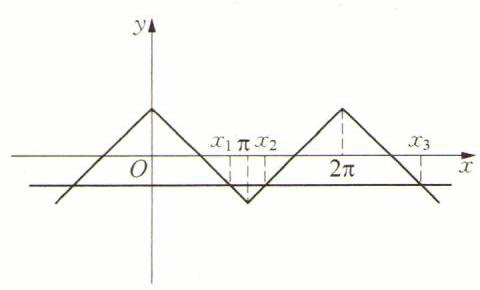
\includegraphics[max width=0.4\textwidth]{images/bo_d29ci7n7aajc738p8c80_51_1024_658_480_290_0.jpg}
\end{center}
\hspace*{3em} 

第 4 题图

【解析】根据已知可得 $y = f\left( x\right)$ 的简图如图所示,则有 ${x}_{1} + {x}_{2} = {2\pi },{x}_{2} + {x}_{3} = {4\pi }$ ,又 ${x}_{2}^{2} = {x}_{1} \cdot  {x}_{3}$ ,可得 ${x}_{2}^{2} =$  $\left( {{2\pi } - {x}_{2}}\right)  \cdot  \left( {{4\pi } - {x}_{2}}\right)$ ,解得 ${x}_{2} = \dfrac{4\pi }{3}$ .

5.【答案】 $t + \dfrac{1}{t},t \in  (1,3\rbrack$

【解析】由函数 $f\left( x\right)$ 的解析式为 $f\left( x\right)  = \left\{  \begin{array}{ll} {2}^{x}, & x \leq  0, \\  {\log }_{2}x, & x > 0. \end{array}\right.$

当 $x \leq  0$ 时, $f\left( x\right)  = {2}^{x} \in  (0,1\rbrack$ ,当 $0 < x \leq  1$ 时, $f\left( x\right)  = {\log }_{2}x \in  ( - \infty ,0\rbrack$ ,当 $x > 1$ 时, $f\left( x\right)  = {\log }_{2}x \in  \left( {0, + \infty }\right)$ ,所以 $f\left( {f\left( x\right) }\right)  = \left\{  \begin{array}{ll} {\log }_{2}{2}^{x}, & x \leq  0, \\  {2}^{{\log }_{2}x}, & 0 < x \leq  1, = \\  {\log }_{2}\left( {{\log }_{2}x}\right) , & x > 1 \end{array}\right.$  $\left\{  \begin{array}{ll} x, & x \leq  1, \\  {\log }_{2}\left( {{\log }_{2}x}\right) , & x > 1. \end{array}\right.$

① 若 $x \leq  1$ ,则方程 $f\left( {f\left( x\right) }\right)  - {\log }_{2}\left( {t - x}\right)  = 0$ 化为 $x = {\log }_{2}\left( {t - x}\right)$ ,即 ${2}^{x} = t - x$ ,且 $1 < t \leq  3$ ;

② 若 $x > 1$ ,则方程 $f\left( {f\left( x\right) }\right)  - {\log }_{2}\left( {t - x}\right)  = 0$ 化为 ${\log }_{2}\left( {{\log }_{2}x}\right)  = {\log }_{2}\left( {t - x}\right)$ ,即 ${\log }_{2}x =$  $t - x$ ,且 $t > 1$ ,于是 ${x}_{1}\text{ 、 }{x}_{2}$ 分别是方程 ${2}^{x} = t - x,{\log }_{2}x = t - x$ 的两个根且 ${x}_{1} \leq  1 <$  ${x}_{2} < t$ ,由于函数 $y = {\log }_{2}x$ 与 $y = {2}^{x}$ 的图象关于直线 $y = x$ 对称,故 ${x}_{1} + {x}_{2} = t,{2}^{{x}_{1}} +$  ${\log }_{2}{x}_{2} = {2t} - \left( {{x}_{1} + {x}_{2}}\right)  = t,\dfrac{1}{2 - \left| {{x}_{1} - 1}\right|  + \left| {{x}_{2} - 1}\right| } = \dfrac{1}{2 + {x}_{1} - 1 + {x}_{2} - 1} = \dfrac{1}{t}$ ,所以 ${2}^{{x}_{1}} + {\log }_{2}{x}_{2} + \dfrac{1}{2 - \left| {{x}_{1} - 1}\right|  + \left| {{x}_{2} - 1}\right| } = t + \dfrac{1}{t},t \in  (1,3\rbrack .$

\section*{17 常用初等函数}

1.【答案】A

【解析】因为 $A = B$ ,且都不是空集,故存在 $a \in  A \cap  B$ ,即 $\left\{  {\begin{array}{l} f\left( a\right)  = 0, \\  f\left( {f\left( a\right) }\right)  = 0 \end{array} \Rightarrow  f\left( {f\left( a\right) }\right)  = }\right.$  $f\left( 0\right)  = 0 \Rightarrow  m = 0.$

令 $f\left( x\right)  = {x}^{2} + {nx} = 0$ . 当 $n = 0$ 时,方程的解为 $x = 0$ ,此时 $A = B = \{ 0\}$ ,符合题意; 当 $n \neq$ 0时, $f\left( x\right)  = {x}^{2} + {nx} = 0$ 的解为 $x = 0$ 或 $x =  - n$ . 由 $B = \{ x \mid  f\left( {f\left( x\right) }\right)  = 0,x \in  \mathbf{R}\}$ ,则 $f\left( x\right)  = {x}^{2} + {nx} = 0$ 或 $f\left( x\right)  = {x}^{2} + {nx} =  - n$ . 因为 $A = B$ ,则 $f\left( x\right)  = {x}^{2} + {nx} =  - n$ 无解, $\Delta  = {n}^{2} - {4n} < 0$ ,所以 $0 < n < 4$ . 综上, $0 \leq  n < 4$ .

所以, $m + n \in  \lbrack 0,4)$ .

2.【答案】 ${C}$

【解析】设 $\left( {{x}_{0},{y}_{0}}\right)$ 为 $y = f\left( x\right)$ 图象的顶点, ${x}_{1}\text{ 、 }{x}_{2}$ 且 ${x}_{1} < {x}_{2}$ 为 $y = f\left( x\right)$ 的两个零点 (若有). 因为 $f\left( {f\left( {-\dfrac{b}{2a}}\right) }\right)  < 0$ ,即 $f\left( {y}_{0}\right)  < 0$ ,故 ${x}_{1},{x}_{2}$ 必存在,且 ${x}_{1} < {y}_{0} < {x}_{2}$ . 故此时显然 $f\left( x\right)$ 恰有两个零点; 再令 $f\left( {f\left( x\right) }\right)  = 0$ ,解得 $f\left( x\right)  = {x}_{1}$ 或 $f\left( x\right)  = {x}_{2}$ ,根据 $y = f\left( x\right)$ 的图象可知,当 $k > {y}_{0}$ 时, $f\left( x\right)  = k$ 有两解; 当 $k = {y}_{0}$ 时, $f\left( x\right)  = k$ 有一解; 当 $k < {y}_{0}$ 时, $f\left( x\right)  = k$ 无解; 因此 $f\left( x\right)  = {x}_{1}$ 无解, $f\left( x\right)  = {x}_{2}$ 有两解,综上, $f\left( {f\left( x\right) }\right)$ 恰有两个零点,满足充分性. 若 $f\left( x\right)$ 有两个零点,则 ${x}_{1}\text{ 、 }{x}_{2}$ 必存在. 由 $f\left( {f\left( x\right) }\right)  = 0$ 得 $f\left( x\right)  = {x}_{1}$ 或 $f\left( x\right)  = {x}_{2}$ ,因为 $f\left( {f\left( x\right) }\right)  = 0$ 也只有两个零点,因此 $f\left( x\right)  = {x}_{1}$ 无解, $f\left( x\right)  = {x}_{2}$ 有两个不等实根,即 ${x}_{1} <$  ${y}_{0} < {x}_{2}$ ,所以 $f\left( {f\left( {-\dfrac{b}{2a}}\right) }\right)  < 0$ ,必要性得证. 故本题是充分必要条件.

3.【答案】(一 ∞,一 2] U [6, 十 ∞)

【解析】由题意得 $g\left( x\right)  = 2{x}^{2} - \left| {x - t}\right| \left( {x - t}\right)  = \left\{  {\begin{array}{ll} 2{x}^{2} - {\left( x - t\right) }^{2}, & x \geq  t, \\  2{x}^{2} + {\left( x - t\right) }^{2}, & x < t \end{array} = }\right.$  $\left\{  {\begin{array}{ll} {x}^{2} + {2tx} - {t}^{2} = {f}_{1}\left( x\right) , & x \geq  t, \\  3{x}^{2} - {2tx} + {t}^{2} = {f}_{2}\left( x\right) , & x < t. \end{array}\text{ 当 }t \leq  0\text{ 时, }x \in  \left\lbrack  {0,2}\right\rbrack  \text{ 时, }g\left( x\right)  = {f}_{1}\left( x\right)  = {x}^{2} + {2tx} - }\right.$  ${t}^{2}$ ,函数 $g\left( x\right)$ 在区间 $\left\lbrack  {0,2}\right\rbrack$ 上是严格减函数,则 $- t \geq  2$ ,即 $t \leq   - 2$ ; 当 $t \geq  2$ 时, $x \in  \lbrack 0$ ,

2] 时, $g\left( x\right)  = {f}_{2}\left( x\right)  = 3{x}^{2} - {2tx} + {t}^{2}$ ,函数 $g\left( x\right)$ 在区间 $\left\lbrack  {0,2}\right\rbrack$ 上是严格减函数,则 $\dfrac{t}{3} \geq$

2,即 $t \geq  6$ ; 当 $0 < t < 2$ 时,当 $x \in  \left\lbrack  {0,2}\right\rbrack$ 时, $g\left( x\right)  = 2{x}^{2} - \left| {x - t}\right| \left( {x - t}\right)  =$  $\left\{  \begin{array}{ll} {x}^{2} + {2tx} - {t}^{2} = {f}_{1}\left( x\right) , & t \leq  x \leq  2, \\  3{x}^{2} - {2tx} + {t}^{2} = {f}_{2}\left( x\right) , & 0 \leq  x < t, \end{array}\right.$ 因为 $- t < 0$ ,因此 $y = {x}^{2} + {2tx} - {t}^{2}$ 在 $\left\lbrack  {t,2}\right\rbrack$ 是单调递增,不合题意. 综上, $t$ 的范围是 $\left( {-\infty , - 2\rbrack \cup \lbrack 6, + \infty }\right)$ .

4.【答案】 $\dfrac{\sqrt{5} + 1}{2}$

【解析】 $f\left( x\right)  = a{x}^{2} + {8x} + 3 = a{\left( x + \dfrac{4}{a}\right) }^{2} + 3 - \dfrac{16}{a}$ .

① 当 $3 - \dfrac{16}{a} > 5$ ,即 $- 8 < a < 0$ 时,如图 1 所示,要使 $\left| {f\left( x\right) }\right|  \leq  5$ 在 $x \in  \left\lbrack  {0,M\left( a\right) }\right\rbrack$ 上恒成立,且 $M\left( a\right)$ 取得最大值,则 $M\left( a\right)$ 只能是 $a{x}^{2} + {8x} + 3 = 5$ 的较小的根,即 $M\left( a\right)  = \dfrac{\sqrt{{2a} + {16}} - 4}{a}.$

② 当 $3 - \dfrac{16}{a} \leq  5$ ,即 $a \leq   - 8$ 时,如图 2 所示,要使 $M\left( a\right)$ 取得最大值,则 $M\left( a\right)$ 只能是 $a{x}^{2} +$  ${8x} + 3 =  - 5$ 的较大的根,即 $M\left( a\right)  = \dfrac{-2\sqrt{4 - {2a}} - 4}{a}$ .

当 $- 8 < a < 0$ 时, $M\left( a\right)  = \dfrac{\sqrt{{2a} + {16}} - 4}{a} = \dfrac{2}{\sqrt{{2a} + {16}} + 4} < \dfrac{1}{2};$

当 $a \leq   - 8$ 时, $M\left( a\right)  = \dfrac{-2\sqrt{4 - {2a}} - 4}{a} = \dfrac{4}{\sqrt{4 - {2a} - 2}} \leq  \dfrac{4}{\sqrt{{20} - 2}} = \dfrac{\sqrt{5} + 1}{2}$ .

所以, $M\left( a\right)$ 的最大值为 $\dfrac{\sqrt{5} + 1}{2}$ .

\begin{center}
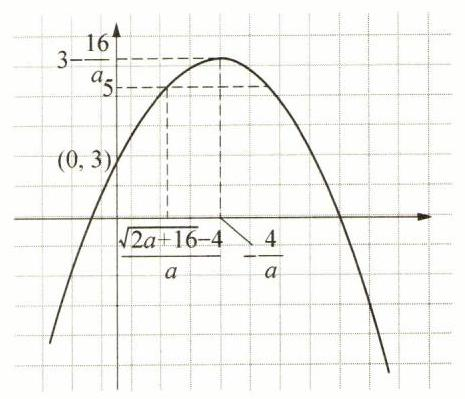
\includegraphics[max width=0.3\textwidth]{images/bo_d29ci7n7aajc738p8c80_53_271_1475_465_399_0.jpg}
\end{center}
\hspace*{3em} 

第 4 题图 1

\begin{center}
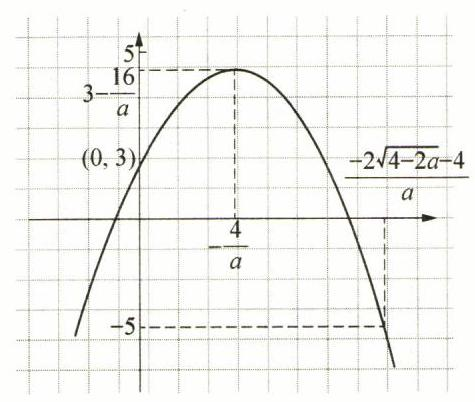
\includegraphics[max width=0.4\textwidth]{images/bo_d29ci7n7aajc738p8c80_53_854_1469_475_402_0.jpg}
\end{center}
\hspace*{3em} 

第 4 题图 2

\section*{18 幂指对函数}

1.【答案】 $- \dfrac{1}{4}$

【解析】 ${\log }_{2}\left( {{\log }_{4}x}\right)  + {\log }_{4}\left( {{\log }_{16}x}\right)  + {\log }_{16}\left( {{\log }_{2}x}\right)  = 0 \Rightarrow  {\log }_{2}\left( {\dfrac{1}{2}{\log }_{2}x}\right)  + \dfrac{1}{2}{\log }_{2}\left( {\dfrac{1}{4}{\log }_{2}x}\right)  +$  $\dfrac{1}{4}{\log }_{2}\left( {{\log }_{2}x}\right)  = 0 \Rightarrow   - 1 + {\log }_{2}\left( {{\log }_{2}x}\right)  + \left( {-1}\right)  + \dfrac{1}{2}{\log }_{2}\left( {{\log }_{2}x}\right)  + \dfrac{1}{4}{\log }_{2}\left( {{\log }_{2}x}\right)  = 0 \Rightarrow$  $\dfrac{7}{4}{\log }_{2}\left( {{\log }_{2}x}\right)  = 2 \Rightarrow  {\log }_{2}\left( {{\log }_{2}x}\right)  = \dfrac{8}{7} \Rightarrow  {\log }_{2}x = {2}^{\dfrac{8}{7}}.$

${\log }_{2}\left( {{\log }_{16}x}\right)  + {\log }_{16}\left( {{\log }_{4}x}\right)  + {\log }_{4}\left( {{\log }_{2}x}\right)  = {\log }_{2}\left( {\dfrac{1}{4}{\log }_{2}x}\right)  + \dfrac{1}{4}{\log }_{2}\left( {\dfrac{1}{2}{\log }_{2}x}\right)  +$  $\dfrac{1}{2}{\log }_{2}\left( {{\log }_{2}x}\right)  =  - 2 + {\log }_{2}\left( {{\log }_{2}x}\right)  - \dfrac{1}{4} + \dfrac{1}{4}{\log }_{2}\left( {{\log }_{2}x}\right)  + \dfrac{1}{2}{\log }_{2}\left( {{\log }_{2}x}\right)  =  - \dfrac{9}{4} +$  $\dfrac{7}{4}{\log }_{2}\left( {{\log }_{2}x}\right)  =  - \dfrac{9}{4} + \dfrac{7}{4} \times  \dfrac{8}{7} =  - \dfrac{1}{4}.$

2.【答案】 $\dfrac{1}{1000}$

【解析】因为 $\lg a + \lg b + \lg c = 0$ ,所以 $\lg {abc} = 0 \Rightarrow  {abc} = 1;{a}^{\dfrac{1}{\lg b + \dfrac{1}{\lg c}}} \times  {b}^{\dfrac{1}{\lg a} + \dfrac{1}{\lg c}} \times  {c}^{\dfrac{1}{\lg a} + \dfrac{1}{\lg b}} = {\left( ab\right) }^{\dfrac{1}{\lg c}} \times$  ${\left( ac\right) }^{\dfrac{1}{\lg b}} \times  {\left( bc\right) }^{\dfrac{1}{\lg a}} = {\left( \dfrac{1}{c}\right) }^{\dfrac{1}{\lg c}} \cdot  {\left( \dfrac{1}{b}\right) }^{\dfrac{1}{\lg b}} \cdot  {\left( \dfrac{1}{a}\right) }^{\dfrac{1}{\lg a}} = {\left( \dfrac{1}{c}\right) }^{{\log }_{c}{10}} \cdot  {\left( \dfrac{1}{b}\right) }^{{\log }_{b}{10}} \cdot  {\left( \dfrac{1}{a}\right) }^{{\log }_{a}{10}} = {c}^{-{\log }_{c}{10}} \cdot  {b}^{-{\log }_{b}{10}}.$  ${a}^{-{\log }_{a}{10}} = {c}^{{\log }_{c}\dfrac{1}{10}} \cdot  {b}^{{\log }_{b}\dfrac{1}{10}} \cdot  {a}^{{\log }_{a}\dfrac{1}{10}} = \dfrac{1}{1000}.$

3.【答案】2

【解析】将 ${2}^{x} = 6 - {3}^{y + 1}$ 代入 ${2}^{x} + {3}^{y + 1} - {2}^{x + 1} \times  {3}^{y} + 2{z}^{2} = 0$ ,得 $\left( {6 - {3}^{y + 1}}\right)  + {3}^{y + 1} - 2 \times  (6 -$  $\left. {3}^{y + 1}\right)  \times  {3}^{y} + 2{z}^{2} = 6 - {12} \times  {3}^{y} + 6 \times  {\left( {3}^{y}\right) }^{2} + 2{z}^{2} = 6\left\lbrack  {{\left( {3}^{y}\right) }^{2} - 2 \times  {3}^{y} + 1}\right\rbrack   + 2{z}^{2} = 6{\left( {3}^{y} - 1\right) }^{2} +$  $2{z}^{2} = 0$ ,故 ${3}^{y} - 1 = 0,z = 0$ ,所以 $y = 0,z = 0$ ,代入 ${2}^{x} = 6 - {3}^{y + 1} = 6 - {3}^{1} = 3$ ,得 $x = {\log }_{2}3$ , ${3}^{\dfrac{1}{x + y + z}} = {3}^{\dfrac{1}{{\log }_{2}3}} = 2.$

4.【答案】 $\left( {\dfrac{1 - n}{2}, + \infty }\right)$

【解析】因为 $f\left( x\right)$ 当 $x \in  ( - \infty ,1\rbrack$ 时有意义,即 $\dfrac{{1}^{x} + {2}^{x} + {3}^{x} + \cdots  + {\left( n - 1\right) }^{x} + {n}^{x}a}{n} >$ 0 在 $x \in  ( - \infty ,1\rbrack$ 时恒成立,即不等式 $- a < {\left( \dfrac{1}{n}\right) }^{x} + {\left( \dfrac{2}{n}\right) }^{x} + \cdots  + {\left( \dfrac{n - 1}{n}\right) }^{x}$ 在 $x \in  ( - \infty$ ,

1] 时恒成立. 记 $g\left( x\right)  = {\left( \dfrac{1}{n}\right) }^{x} + {\left( \dfrac{2}{n}\right) }^{x} + \cdots  + {\left( \dfrac{n - 1}{n}\right) }^{x},x \in  ( - \infty ,1\rbrack$ ,显然 $g\left( x\right)$ 为减函数,所以 $g{\left( x\right) }_{\min } = g\left( 1\right)  = \dfrac{1}{n} + \dfrac{2}{n} + \cdots  + \dfrac{n - 1}{n} = \dfrac{n - 1}{2}$ ,故 $- a < g{\left( x\right) }_{\min } = \dfrac{n - 1}{2} \Rightarrow  a >$  $\dfrac{1 - n}{2}$

5.【答案】4

【解析】因为函数经过 $P\text{ 、 }Q$ 两点,所以 $\dfrac{{2}^{p}}{{2}^{p} + {ap}} = \dfrac{6}{5} \Rightarrow  5 \cdot  {2}^{p} = 6 \cdot  {2}^{p} + {6ap} \Rightarrow  {2}^{p} =  - {6ap}$ ,同理 ${2}^{q} =  - \dfrac{1}{6}{aq}$ . 因为 ${2}^{p + q} = {16pq}$ ,所以 ${2}^{p + q} = {a}^{2}{pq} = {16pq} \Rightarrow  a = 4$ (负舍).

6.【答案】C

【解析】令 $t = {2}^{x} + {2}^{-x} = {2}^{x} + \dfrac{1}{{2}^{x}}$ ,因为 $x \in  \left\lbrack  {-1,1}\right\rbrack$ ,则 ${2}^{x} \in  \left\lbrack  {\dfrac{1}{2},2}\right\rbrack$ ,所以 $t \in  \left\lbrack  {2,\dfrac{5}{2}}\right\rbrack$ . 因为 ${t}^{2} = {\left( {2}^{x} + {2}^{-x}\right) }^{2} = {4}^{x} + {4}^{-x} + 2$ ,则 ${4}^{x} + {4}^{-x} = {t}^{2} - 2$ ,所以 $f\left( x\right)  = {t}^{2} + {kt} - 2$ ,构造函数 $h\left( t\right)  = {t}^{2} + {kt} - 2$ ,其中 $t \in  \left\lbrack  {2,\dfrac{5}{2}}\right\rbrack$ . 由 $h\left( t\right)  = {t}^{2} + {kt} - 2 > 0$ ,可得 $k > \dfrac{2}{t} - t$ ,由于

函数 $y = \dfrac{2}{t} - t$ 在区间 $\left\lbrack  {2,\dfrac{5}{2}}\right\rbrack$ 上单调递减,则 ${y}_{\max } =  - 1$ ,可得 $k >  - 1$ . 二次函数 $h\left( t\right)  = {t}^{2} +$  ${kt} - 2$ 的对称轴为直线 $t =  - \dfrac{k}{2} < \dfrac{1}{2}$ ,所以 $t \in  \left\lbrack  {2,\dfrac{5}{2}}\right\rbrack$ 时, $h{\left( t\right) }_{\min } = h\left( 2\right)  = {2k} + 2,h{\left( t\right) }_{\max } =$  $h\left( \dfrac{5}{2}\right)  = \dfrac{5}{2}k + \dfrac{17}{4}$ . 由于以 $f\left( {x}_{1}\right) \text{ 、 }f\left( {x}_{2}\right) \text{ 、 }f\left( {x}_{3}\right)$ 为长度的线段都可以围成三角形,所以, $2\left( {{2k} + 2}\right)  > \dfrac{5}{2}k + \dfrac{17}{4}$ ,解得 $k > \dfrac{1}{6}$ . 因此,实数 $k$ 的取值范围是 $\left( {\dfrac{1}{6}, + \infty }\right)$ .

7.【答案】D

【解析】由已知 $4 - {2x} > 0$ 得 $x < 2$ ,又不等式 ${\log }_{2}\left( {4 - {2x}}\right)  < {a}^{2}{x}^{2} + {ax} + 4$ 的解集是 $A$ , 不等式 ${\log }_{2}\left( {4 - {2x}}\right)  \geq  {a}^{2}{x}^{2} + {ax} + 4$ 的解集是 $B$ ,所以 $A \cup  B = \{ x \mid  x < 2\}$ . 若 $A \subset  B$ , 则 $B = \{ x \mid  x < 2\}$ ,当 $x \rightarrow   - \infty$ 时,若 $a \neq  0$ ,显然 ${\log }_{2}\left( {4 - {2x}}\right)  < {a}^{2}{x}^{2} + {ax} + 4$ . 故 $B$ 不可能是 $\{ x \mid  x < 2\}$ ；若 $a = 0$ 时, ${\log }_{2}\left( {4 - {2x}}\right)  \geq  {a}^{2}{x}^{2} + {ax} + 4$ 为 ${\log }_{2}\left( {4 - {2x}}\right)  \geq  4$ ,解得 $x \leq   - 6$ ,即 $B = \{ x \mid  x \leq   - 6\}  \neq  \{ x \mid  x < 2\}$ ,综上,故 ① 错误.

因为 ${a}^{2}{x}^{2} + {ax} + 4 = {\left( ax + \dfrac{1}{2}\right) }^{2} + \dfrac{15}{4} \geq  \dfrac{15}{4}$ ,当 $x \in  \left\lbrack  {-4,0}\right\rbrack$ 时, ${\log }_{2}\left( {4 - {2x}}\right)  \in  \lbrack 2$ , $\left. {{\log }_{2}{12}}\right\rbrack$ ,因为 ${\log }_{2}{12} < \dfrac{15}{4}$ ,即当 $x \in  \left\lbrack  {-4,0}\right\rbrack$ 时 ${\log }_{2}\left( {4 - {2x}}\right)  < {a}^{2}{x}^{2} + {ax} + 4$ 恒成立, 所以对任意的 $a \in  \mathbf{R}$ ,都有 $\left\lbrack  {-4,0}\right\rbrack   \subset  A$ ,故 ② 正确.

8.【答案】D

【解析】对于 ①,当 $a = \dfrac{1}{4},b = 2$ 时, ${\ln }^{ + }\left( {ab}\right)  = {\ln }^{ + }\dfrac{1}{2} = 0,{\ln }^{ + }a + {\ln }^{ + }b = {\ln }^{ + }\dfrac{1}{4} + {\ln }^{ + }2 = \ln 2$ , 故命题 ① 错误.

对于 ②,当 $0 < a < 1,b > 0$ 时,有 $0 < {a}^{b} < 1$ ,从而 ${\ln }^{ + }\left( {a}^{b}\right)  = 0,b{\ln }^{ + }a = b \times  0 = 0$ ,所以 $\mathop{\ln }\limits^{ + }\left( {a}^{b}\right)  = b\mathop{\ln }\limits^{ + }a$ ; 当 $a \geq  1,b > 0$ 时,有 ${a}^{b} > 1$ ,从而 $\mathop{\ln }\limits^{ + }\left( {a}^{b}\right)  = \ln {a}^{b} = b\ln a,b\mathop{\ln }\limits^{ + }a =$  $b\ln a$ ,所以 ${\ln }^{ + }\left( {a}^{b}\right)  = b{\ln }^{ + }a$ . 所以当 $a > 0,b > 0$ 时,命题 ② 正确.

对于 ③,由 “正对数” 的定义知, ${\ln }^{ + }x \geq  0$ 且 ${\ln }^{ + }x \geq  \ln x$ .

当 $0 < a < 1,0 < b < 1$ 时, ${\ln }^{ + }a - {\ln }^{ + }b = 0 - 0 = 0$ ,而 ${\ln }^{ + }\left( \dfrac{a}{b}\right)  \geq  0$ ,则 ${\ln }^{ + }\left( \dfrac{a}{b}\right)  \geq  {\ln }^{ + }a -$  ${\ln }^{ + }b$ ；当 $a \geq  1,0 < b < 1$ 时,有 $\dfrac{a}{b} > 1,{\ln }^{ + }a - {\ln }^{ + }b = {\ln }^{ + }a - 0 = \ln a$ ,而 ${\ln }^{ + }\left( \dfrac{a}{b}\right)  = \ln \dfrac{a}{b} =$  $\ln a - \ln b$ ,因为 $\ln b < 0$ ,则 ${\ln }^{ + }\left( \dfrac{a}{b}\right)  \geq  {\ln }^{ + }a - {\ln }^{ + }b$ . 当 $0 < a < 1,b \geq  1$ 时,有 $0 < \dfrac{a}{b} <$ 1. ${\ln }^{ + }a - {\ln }^{ + }b = 0 - {\ln }^{ + }b =  - \ln b \leq  0$ ,而 ${\ln }^{ + }\left( \dfrac{a}{b}\right)  = 0$ ,则 ${\ln }^{ + }\left( \dfrac{a}{b}\right)  \geq  {\ln }^{ + }a - {\ln }^{ + }b$ . 当 $a \geq  1$ , $b \geq  1$ 时, $\underset{a}{{\ln }^{ + }a} - {\ln }^{ + }b = \ln a - \ln b = \ln \dfrac{a}{b}$ ,则 ${\ln }^{ + }\left( \dfrac{a}{b}\right)  \geq  {\ln }^{ + }a - {\ln }^{ + }b$ . 故命题 ③ 正确.

对于 ④,由“正对数” 的定义知,当 ${x}_{1} \leq  {x}_{2}$ 时,有 ${\ln }^{ + }{x}_{1} \leq  {\ln }^{ + }{x}_{2}$ . 当 $0 < a < 1,0 < b <$ 1 时,有 $0 < a + b < 2$ ,所以 ${\ln }^{ + }\left( {a + b}\right)  \leq  {\ln }^{ + }a + {\ln }^{ + }b + {\ln }^{ + }2$ ; 当 $a \geq  1,0 < b < 1$ 时, 而 ${\ln }^{ + }\left( {a + b}\right)  = \ln \left( {a + b}\right)  < \ln \left( {a + a}\right)  = \ln {2a} = \ln a + 0 + \ln 2 \leq  {\ln }^{ + }a + {\ln }^{ + }b + {\ln }^{ + }2$ ; 当 $0 <$  $a < 1,b \geq  1$ 时,同理; 当 $a \geq  1,b \geq  1$ 时, ${\ln }^{ + }\left( {a + b}\right)  = \ln \left( {a + b}\right) ,{\ln }^{ + }a + {\ln }^{ + }b + {\ln }^{ + }2 =$  $\ln a + \ln b + \ln 2 = \ln \left( {2ab}\right)$ ,易知 ${2ab} \geq  a + b$ ,从而 ${\ln }^{ + }\left( {a + b}\right)  \leq  {\ln }^{ + }a + {\ln }^{ + }b + {\ln }^{ + }2$ ,故命题 ④ 正确.

所以, 正确的命题是 ②③④.

9.【答案】A

【解析】令函数 $g\left( x\right)  = f\left( x\right)  - \dfrac{1}{2} = \dfrac{{3}^{x}}{1 + {3}^{x}} - \dfrac{1}{2} = \dfrac{{3}^{x} - 1}{2\left( {1 + {3}^{x}}\right) } = \dfrac{1}{2} - \dfrac{1}{1 + {3}^{x}}$ ,易知 $g\left( x\right)$ 为严格单调递增函数, 且为奇函数, 图象关于点 ( 0, 0 ) 对称, 如图 1 所示.

对于 ①,因为 ${x}_{1} + {x}_{2} + {x}_{3} = 0$ ,且 ${x}_{1} \cdot  {x}_{2} \cdot  {x}_{3} > 0$ ,则 ${x}_{3} =  - \left( {{x}_{1} + {x}_{2}}\right)$ ,不妨设 ${x}_{1} < 0$ , ${x}_{2} < 0,{x}_{3} > 0$ ,则点 $A\left( {{x}_{1} + {x}_{2},f\left( {{x}_{1} + {x}_{2}}\right) }\right)$ ,此时直线 ${OA}$ 的方程为 $y = \dfrac{f\left( {{x}_{1} + {x}_{2}}\right) }{{x}_{1} + {x}_{2}}x$ , 可得 $g\left( {x}_{1}\right)  < \dfrac{g\left( {{x}_{1} + {x}_{2}}\right) }{{x}_{1} + {x}_{2}}{x}_{1},g\left( {x}_{2}\right)  < \dfrac{g\left( {{x}_{1} + {x}_{2}}\right) }{{x}_{1} + {x}_{2}}{x}_{2}$ ,则 $g\left( {x}_{1}\right)  + g\left( {x}_{2}\right)  <$  $\dfrac{g\left( {{x}_{1} + {x}_{2}}\right) }{{x}_{1} + {x}_{2}}{x}_{1} + \dfrac{g\left( {{x}_{1} + {x}_{2}}\right) }{{x}_{1} + {x}_{2}}{x}_{2} = g\left( {{x}_{1} + {x}_{2}}\right)$ ,又由 $g\left( {x}_{3}\right)  = g\left\lbrack  {-\left( {{x}_{1} + {x}_{2}}\right) }\right\rbrack   =  - g\left( {{x}_{1} + }\right.$  $\left. {x}_{2}\right)$ ,所以 $g\left( {x}_{1}\right)  + g\left( {x}_{2}\right)  + g\left( {x}_{3}\right)  < 0$ ,即 $f\left( {x}_{1}\right)  - \dfrac{1}{2} + f\left( {x}_{2}\right)  - \dfrac{1}{2} + f\left( {x}_{3}\right)  - \dfrac{1}{2} < 0$ ,即 $f\left( {x}_{1}\right)  + f\left( {x}_{2}\right)  + f\left( {x}_{3}\right)  < \dfrac{3}{2}$ ,所以 ① 正确.

对于 ②, 分析思路同 ①, 所以 ② 正确.

\begin{center}
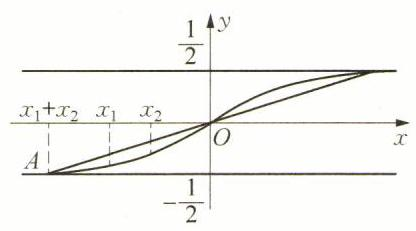
\includegraphics[max width=0.3\textwidth]{images/bo_d29ci7n7aajc738p8c80_57_318_534_416_231_0.jpg}
\end{center}
\hspace*{3em} 

第 9 题图 1

\begin{center}
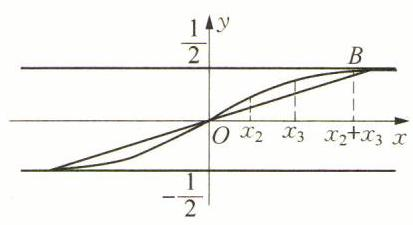
\includegraphics[max width=0.3\textwidth]{images/bo_d29ci7n7aajc738p8c80_57_865_540_413_225_0.jpg}
\end{center}
\hspace*{3em} 

第 9 题图 2

10.【答案】 $\left\lbrack  {2 + 2\sqrt{3},4 + 4\sqrt{2}}\right\rbrack$

【解析】原式可化简得 ${\log }_{a}^{2}x - 4{\log }_{a}x + {\log }_{a}^{2}y - 4{\log }_{a}y = 8$ ,令 $m = {\log }_{a}x,n = {\log }_{a}y$ ,则有 ${n}^{2} + {m}^{2} - {4n} - {4m} = 8$ ,以及 ${\log }_{a}\left( {xy}\right)  = n + m$ . 因为 $a > 1,x \geq  1,y \geq  1$ ,所以 $n \geq  0$ , $m \geq  0$ ,则由 ${n}^{2} + {m}^{2} - {4n} - {4m} = 8$ 得 ${\left( n - 2\right) }^{2} + {\left( m - 2\right) }^{2} = {4}^{2}\left( {n \geq  0,m \geq  0}\right)$ ,表示以 $(2$ , 2)为圆心,半径为 4 的圆在第一象限的部分(包括与 $x$ 、 $y$ 轴正半轴的交点). 令 ${\log }_{a}\left( {xy}\right)  =$  $n + m = z$ ,设 $n - 2 = 4\cos \theta ,m - 2 = 4\sin \theta$ ,因为 $n \geq  0,m \geq  0$ ,所以 $\theta  \in  \left\lbrack  {-\dfrac{\pi }{6},\dfrac{2\pi }{3}}\right\rbrack$ ,则 $z = n + m = 2 + 4\cos \theta  + 2 + 4\sin \theta  = 4 + 4\sqrt{2}\sin \left( {\theta  + \dfrac{\pi }{4}}\right)  \in  \left\lbrack  {2 + 2\sqrt{3},4 + 4\sqrt{2}}\right\rbrack$ ,即 ${\log }_{a}\left( {xy}\right)$ 的取值范围为 $\left\lbrack  {2 + 2\sqrt{3},4 + 4\sqrt{2}}\right\rbrack$ .

\section*{三角}

\section*{19 扇形的弧长、面积公式}

1. $4 + \dfrac{5\pi }{2}$ 2. A 3. 16 4. C 5.445 米

\section*{20 任意角的三角比}

1. D 2. 11 3. B 4. 0 5. $\dfrac{2\pi }{7}$ 6. $\dfrac{\sqrt{2}\pi }{2}7 \cdot  \dfrac{\pi }{4}$ 8. A 9. $\pm  1$

\section*{21 三角恒等式}

1. C 2. $\dfrac{2 + \sqrt{2}}{8}$ 3. $\sqrt{5} - 2$ 4. $2\sqrt{2}$ 5. A 6. $\cos \alpha  - \cos \beta  = \dfrac{1}{3}$ 7. D 8. B 9. $( - \infty ,1\rbrack$

\section*{22 解三角形}

5. $\dfrac{2\sqrt{39}}{3}$

\section*{23 三角函数的性质}

1.(-2,0)2. $\left( {0,\dfrac{1}{12}}\right\rbrack   \cup  \left\lbrack  {\dfrac{1}{6},\dfrac{7}{12}}\right\rbrack$ 3. 16 4. 3 5. $\left\lbrack  {\dfrac{2\pi }{3},\dfrac{10\pi }{3}}\right)$ 6. C 7. 0 8. D 9. $\left\lbrack  {0,\dfrac{2\pi }{3}}\right\rbrack$ 10. $\left\lbrack  {\dfrac{7}{25},\dfrac{4}{5}}\right\rbrack$ 12. $\dfrac{4037}{2}\pi$ 15. $\left\{  {\dfrac{\pi }{12},\dfrac{\pi }{3},\dfrac{7\pi }{12},\dfrac{5\pi }{6}}\right\}$

\section*{向量}

\section*{24 向量的几何意义: 投影}

5. $\left( {-\dfrac{1}{2},1}\right\rbrack$ 8. $\left\lbrack  {3 - \sqrt{3},3 + \sqrt{3}}\right\rbrack$

\section*{25 向量 “三化” 原则}

1. A 2. 2 3.-24.-35. B 6. $\dfrac{2}{5}\overrightarrow{a} + \dfrac{1}{5}\overrightarrow{b}$ 7. $- \dfrac{1}{2}$ 8. $\sqrt{3} + 1$ 9. $\dfrac{1}{3}$ 10. 1

11. 4 12. -4 13. 1

\section*{26 向量极化恒等式}

1.(-1,8) 2. $\left\lbrack  {5 - 2\sqrt{13},0}\right\rbrack$ 3. $\left\lbrack  {-\dfrac{9}{4}, - 2}\right\rbrack$ 4. $\left\lbrack  {6 - 4\sqrt{6},8 + 8\sqrt{2}}\right\rbrack$ 5. $- 46$ . A 7. 3 27 “奔驰”定理 1.3 2.5 :13. B 4. B 5. 14 28 三角形的 “四心” 1. $\dfrac{4}{5}$ 2. A 3. C 4. A 5. A 6. C 7. C 8. B 9. A 10. A

\section*{29 等和线}

1. D 2. D 3. $\dfrac{2}{3}$ 4. $\left\lbrack  {3,4}\right\rbrack$ 5. C 6. B

\section*{立体几何}

\section*{30 位置关系}

1. B 2. ${s}_{1}//{s}_{2}$ ,且 ${t}_{1}$ 与 ${t}_{2}$ 相交(或者 ${t}_{1}//{t}_{2}$ , ${s}_{1}$ 与 ${s}_{2}$ 相交) 3. D 4. B 5. ${40}^{ \circ  } < \theta  < {50}^{ \circ  }$ 6. ①③

\section*{31 截面问题}

1. $\dfrac{9}{2}$ 2. ②④ 3. ①② 4. ①②③ 5. ①④ 6. ②③④ 7. BC

\section*{32 化折为直}

1．A 2．A 3．B 4．B 5．C 6．D 7．C

\section*{33 最大角和最小角问题}

1. B 2. B 3. $\dfrac{2\sqrt{5}}{5}$ 4. B 5. C 6. $\dfrac{\sqrt{3}}{3}$ 7. A

\section*{34 空间想象力}

6. $\left( {0,\sqrt{6} + \sqrt{2}}\right)$ 7. D 8. $\dfrac{\sqrt{3} - \sqrt{6}}{3}$

\section*{35 球体相关}

5. $\dfrac{\sqrt{30}\pi }{3}$ 6. $\dfrac{3\pi }{2}7 \cdot  \dfrac{1}{2};\dfrac{2 + \sqrt{2}}{2}$

\section*{36 最值问题}

1. C 2. $\left\lbrack  {\dfrac{8\sqrt{2} - 8}{3},\dfrac{8\sqrt{2} + 8}{3}}\right\rbrack$ 4. $\dfrac{\sqrt{3} + 1}{2}$ 5. $\dfrac{{11}\sqrt{5}}{25}$ 6. $\sqrt{3};\dfrac{\sqrt{3}}{3}$

\section*{圆锥曲线}

\section*{37 定义与几何性质}

1. $\left\lbrack  {1,\sqrt{2}}\right\rbrack$ 2. 11 3. $2\mathbf{4}.{C}$ 5. $a \geq  1\mathbf{6}.\sqrt{2}\mathbf{7}.{C}\mathbf{8}.\mathbf{4}\mathbf{9}.\mathbf{1}\mathbf{{10}}.\mathbf{1}$

\section*{38 离心率}

1. $\left( {\dfrac{-1 + \sqrt{5}}{2},1}\right)$ 2. $\dfrac{2\sqrt{26}}{13}$ 3. $\left\lbrack  {\dfrac{\sqrt{3}}{3},\dfrac{\sqrt{2}}{2}}\right\rbrack$ 4. $\left\lbrack  {\sqrt{3} - 1,\dfrac{\sqrt{6}}{3}}\right\rbrack$

9. $\left( {1,\sqrt{2} + 1}\right)$ 10. 2

\section*{39 点的存在性问题}

1. $\left\lbrack  {-\dfrac{1}{2},1}\right\rbrack$ 2. $\left\lbrack  {-2,2}\right\rbrack  3 \cdot  \left\lbrack  {-1,1}\right\rbrack  4$  $\sqrt{3}, - 2 + \sqrt{3}\rbrack  \cup  \left\lbrack  {2 - \sqrt{3},2 + \sqrt{3}}\right\rbrack  $ 8. D 9. $\left( {-\infty , - \dfrac{\sqrt{5}}{2}}\right)  \cup  \left\lbrack  {\dfrac{\sqrt{5}}{2}, + \infty }\right) $ 10. $\left\lbrack  {-\dfrac{6}{5},0}\right\rbrack$

\section*{40 位置关系}

1. D 2. 2 3. $\sqrt{2}$ 4. $2 < r < 4$ 5. $\dfrac{1}{2}$ 6. C 7. 2 8. $\left\lbrack  {\dfrac{\pi }{4},\dfrac{\pi }{3}}\right\rbrack   \cup  \left\lbrack  {\dfrac{2\pi }{3},\dfrac{3\pi }{4}}\right\rbrack  $ 9. $\dfrac{\sqrt{21}}{3}$ 10. 1

\section*{41 对称与旋转问题}

1. $\dfrac{\sqrt{15}}{3}$ 2. $\left( {-\infty ,1}\right)$ 3. $\left( {1,\sqrt{2}}\right\rbrack$ 4. $3\sqrt{2}$ 5. $\left( {\dfrac{3}{4}, + \infty }\right)$ 6. $\sqrt{2}7.\left( {2 + \sqrt{2}}\right) \pi$ 8. 2 9. $2\sqrt{2} + 1$ 10. $8\sqrt{2}$

\section*{42 曲线的参数方程与曲线系方程}

1. C 2. C 3. B 4. $\left\lbrack  {-\sqrt{2} - 2,2 - \sqrt{2}}\right\rbrack  $ 5. D 6. $\sqrt{6}7.\left( {\dfrac{1}{c} - \dfrac{1}{b}}\right) x + \left( {\dfrac{1}{p} - \dfrac{1}{a}}\right) y = 0$ 8. ${2x} - {3y} = 0\mathbf{9}.\left( {0,1}\right) ,\left( {\dfrac{1}{2},\dfrac{3}{2}}\right)$

\section*{43 新定义问题}

1.4 2. A 3. ${32} + {16\pi }$ 4. $\left( {\sqrt{5},2\sqrt{2} + \sqrt{5}}\right.$ 5. D 6. A 7. ②③ 8. A 9. C 10. ②③

\section*{44 曲线中的定点定值与向量问题}

D 2. $\left( {\sqrt{2}, + \infty }\right) $ 3. $\left( {\dfrac{5}{4},0}\right) $ 4. $\left\lbrack  {0,\sqrt{5}}\right\rbrack  $ 5. $\sqrt{2}$ 6. $8\mathbf{7}.{x}^{2} + \dfrac{{y}^{2}}{3} = 1\left( {y \neq  0}\right)$ 8. $\dfrac{3}{2}\sqrt{3}$ 9. 2 10. $\left( {{20}, + \infty }\right) $ 11. 0 12. $\left\lbrack  {\dfrac{1}{2},1}\right)$

\section*{45 曲线中的距离问题}

1. $\left\lbrack  {2 - \sqrt{3},2 + \sqrt{3}}\right\rbrack  $ 2. 18 $3.24.\lbrack 4, + \infty ){5.100} + {25}\sqrt{3}6.\sqrt{6}7.2$ 或 4

8. $\left\lbrack  {\dfrac{4}{5},\dfrac{{17} + 8\sqrt{3}}{3}}\right)$ 10. $2\sqrt{2} - 5$ 11. $\lbrack 2\sqrt{5} + 2,8)$

\section*{46 面积问题}

1.1 2. A 3. 1 4. A 5. 2 6. 4 7. D 8. $\left( {3 - 2\sqrt{7},3 - 2\sqrt{3}}\right\rbrack   \cup  \left\lbrack  {3 + 2\sqrt{3},3 + }\right.$  $2\sqrt{7}$ )9. ${27}{10}.{B}{11}.\dfrac{{32}\sqrt{3}}{9}{12}.\sqrt{2}{13}.9$

\section*{数列}

\section*{47 数列的概念}

1. 80 2. 18 3. C 4. ②③ 5. D 6. B 7. D 8. C 9.1078 10. $\sqrt{3}{11} \cdot  \dfrac{n\left( {n - 1}\right) }{2}\pi$

\section*{48 等差等比数列}

1．B 2．4 3．C 4．D 5．A 6．B 7．A 8．2 $\sqrt{2}\mathbf{9}$ ． $\dfrac{11}{6}\mathbf{{10}}$ ． $\dfrac{9}{5}\mathbf{{11}}$ ．3＋2 $\sqrt{2}$ 12. $\dfrac{5 + \sqrt{85}}{6}$ 13. D 14. 11302 15. ①③④

\section*{49 递推数列求通项}

1. 1980 2. ${2}^{1014}{3.3}{4.}\dfrac{2\sqrt{3}}{3}\mathbf{5}{.81}\mathbf{6}$ . A7. B8. 0

\section*{${50}{a}_{n}$ 与 ${\mathbf{S}}_{n}$ 之间的关系及应用}

1. $\dfrac{3}{2}$ 2. 2021 3. ${a}_{n} = 1 - {3}^{n}$ 6. $\left( {-\dfrac{3}{4},\dfrac{11}{4}}\right)$ 7. $\dfrac{505}{2021}$

\section*{51 数列求和}

2. $\dfrac{2023}{2}$ D $6 \cdot  {3}^{2021} - 37 \cdot   - 28 \cdot  {C}$

\section*{52 数列的函数性质}

1. $\left( {0,\dfrac{1}{2}}\right)  \cup  \left( {2, + \infty }\right) $ 2. 5 3. ②③ 4. $\dfrac{1}{1 - q}\left( {0 < q < 1}\right) $ 5. $\left( {0,\dfrac{1}{3}}\right)$

\section*{53 数列新定义}

1. D 2.4 3. 6 4. ③④ 5. 4 6. B 7.7274 8. 679055 9. B 10. $1 + \dfrac{1}{2n}$ 11. $\left( {-\infty ,\dfrac{1}{2}}\right\rbrack   \cup  \left( {\dfrac{9}{2}, + \infty }\right) $ 12. $\dfrac{{m}^{n} - 1}{2}{13.143}{14.512}{15.}{C}{16.}{B}$

\section*{54 数列与不等关系}

1. 111 2. 128 3. A 4. $\left\lbrack  {-5, - 3}\right\rbrack$ 5. $\dfrac{1}{2016}$ 6. $\left\lbrack  {-7,\dfrac{29}{4}}\right\rbrack$ 7. $\dfrac{1}{27}$ 8. $\dfrac{1}{3}$ 9. $\left( {0,\dfrac{1}{2}}\right)  \cup  \left( {2, + \infty }\right) $ 10. $\sqrt{2}{11.25}{12}$ . A 13. ${512}{14}.m = 1$ 或 2 15. C

\section*{导数}

\section*{55 导数的定义与计算}

1. A 2. A 3. $\dfrac{\pi }{8}$ 4. (1) $\left( {{6x} + 2}\right) \cos x - \left( {3{x}^{2} + {2x} + 1}\right) \sin x$ ; (2) $\dfrac{9}{2}{x}^{\dfrac{1}{2}} - \dfrac{1}{2}{x}^{-\dfrac{3}{2}} +1$ (3) $\left( {{2}^{x}\ln 2}\right) \cos x - {2}^{x}\sin x - 3{\log }_{3}x - 3{\log }_{3}{e}$ ; (4) $- \dfrac{1}{3}{\cos }^{-\dfrac{2}{3}}\left( {{2}^{x} + x}\right)  \cdot  \sin \left( {{2}^{x} + x}\right)$ . $\left( {{2}^{x}\ln 2 + 1}\right) ;\left( 5\right) \dfrac{{\left( x - 1\right) }^{2}}{{{e}}^{x}}\sin 2\left( \dfrac{1 + {x}^{2}}{{{e}}^{x}}\right) $ 5. BC

\section*{56 切线}

1. $y = \dfrac{1}{{e}}x;y =  - \dfrac{1}{{e}}x$ 2. $\left( {-\infty ,0}\right)  \cup  \left( {8, + \infty }\right) $ 3.24. $\left( {0,1}\right) $ 5. $\dfrac{3}{2}{{e}}^{\dfrac{2}{3}}$

6. ABD 7. $\left\lbrack  {\dfrac{1}{2}{{e}}^{-3}, + \infty }\right) $ 8. $\dfrac{3}{2};a \geq  \dfrac{3}{2}$ 9. ${C}$

\section*{57 切线的应用}

1. $\sqrt{2}\mathbf{2}$ .23. $\mathbf{C}\mathbf{4}.\sqrt{5}\mathbf{5}$ . B 6. B 7. B

\section*{58 导数与单调性}

1．C 2．C 3．(-∞,5 1 4．A 5．B 6．D 7．B 8．C 9．- $\dfrac{1}{2{e}}$ 10．C

\section*{59 利用导数研究图象}

1. $a > \dfrac{2}{{e}}$ 或 $a <  - \dfrac{2}{{e}}$ 2. B 3. $\left( {-\dfrac{5}{{{e}}^{2}},0}\right) $ 4. B 5. B 6. $\left( {0,1}\right) $ 7. $\left( {-\infty , - \dfrac{1}{2}}\right)  \cup$  $\left( {\dfrac{1}{2}, + \infty }\right)  \cup  \{ 0\}$

\section*{60 导数与极值}

6. $a \leq  \dfrac{{{e}}^{2}}{4}$ 或 $a = \dfrac{{{e}}^{3}}{9}$ 7. $\left( {\dfrac{1}{{e}},1}\right) $ 8. ${D}9.(4$ , 5) 10. B 11. C

\section*{61 有解恒成立问题}

1. C 2. $\left\lbrack  {{e}, + \infty }\right\rbrack  $ 3. $\left( {\dfrac{1}{3{e}},\dfrac{4}{3{{e}}^{2}}}\right\rbrack  $ 4. $\left\lbrack  {0,{{e}}^{-2}}\right\rbrack  $ 5. C 6. $( - \infty ,4 + \ln 4\rbrack $ 7. A 8. $( - \infty$ . 1] 9. $\left( {\dfrac{2}{{e}}, + \infty }\right)$

\section*{62 导数的实际应用}

1. 200 2. C 3. $\dfrac{\sqrt{3}}{20}v4 \cdot  \dfrac{\sqrt{2}}{2}{5.6}$ 时

\section*{63 导函数的性质}

1. ① 2. A 3. BC 4. (0,1) (答案不唯一) 5. ABC

\section*{64 函数同构}

1. B 2. $\lbrack  - {e}, + \infty )$ 3. $\dfrac{4}{{{e}}^{2}} + 4$ 4. e 5. B 6. $\lbrack 1, + \infty )$

65 导数综合习题

1.C 2.B 3. $\left\lbrack  {\dfrac{1}{{e}},\dfrac{9}{{{e}}^{3}}}\right) $ 4.12 5. $\dfrac{1}{{e}}$ 6. $\dfrac{1}{2{e}}$ 7. $- 1$ 8. D

\section*{其他}

\section*{66 复数}

1. A 2. C 3. B 4. $6\sqrt{6}\mathbf{5}.\sqrt{2}\mathbf{6}.\dfrac{7}{2}\mathbf{7}.\left( {\dfrac{\sqrt{3}}{3}, + \infty }\right) \mathbf{8}.{C}\mathbf{9}.\left( {-1,1}\right)  \cup  \{  - 3\}$ 10. 2 11. ①②③

\section*{67 排列组合}

1.78 2.78 3.58024 4. ${3}^{n} - {2}^{n} - {2n} - 1$ 5. 7 或 14 6. D 7. B 8. C 9.36 10. 33 11. C 12. 155

\section*{68 概率统计}

1. 0.985 2. $\dfrac{7}{27}$ 3. C 4. $\dfrac{5}{28}$ 5. $\dfrac{1}{54}$ 6. A 7. ③ 8. $\dfrac{3}{5}$ 9. ${p}_{n} = \dfrac{1}{2}{\left( -\dfrac{2}{3}\right) }^{n - 1} + \dfrac{1}{2}$

10. D 11. 18. 4
\end{document}